% -*-coding: utf-8 -*-

\def\usewhat{pdflatex}    % 你喜欢哪种编译方式,pdflatex dvipdfmx dvipspdf xelatex yap

%定义xelatex的中间临时变量,若\usewhat为xelatex时,后面执行xelatx的相关选项
\def\atempxetex{xelatex} %这一项无需改动
%input "reference\reference.bib" %for winedt users
\def\version{1.9.1.20090315}         % 该变量仅用于模板文件的版本号控制,新的论文规范从1.9开始;

\def \xuewei {Doctor}   % 定义学位 博士
%\def \xuewei {Master}    % 硕士

\def\oneortwoside{twoside} %定义单双面打印,只对硕士学位论文有效;
%\def\oneortwoside{oneside} % 硕士单面打印

\def\xueke{Engineering} % 定义学科 工学
%\def\xueke{Science}      % 理学
%\def\xueke{Management}   % 管理学
%\def\xueke{Arts}         % 艺术学

% ��xelatex�����UTF8�ļ�������ÿ���ļ���ָ���ַ�����;
% main.tex���ֶ��ƶ���\atemp��\usewhat������
\ifx\atempxetex\usewhat 
\XeTeXinputencoding "gbk"
\fi

% ˶������ ��һЩ����

% ������ʹ������
\makeatletter
\@tempcnta=128
\loop \catcode\@tempcnta=13 \ifnum\@tempcnta<255 \advance \@tempcnta \@ne
\repeat
\makeatother

\newif\ifxueweidoctor %���������
\newif\ifxueweimaster
\def\temp{Doctor}
\ifx\temp\xuewei
  \xueweidoctortrue  \xueweimasterfalse
\fi
\def\temp{Master}
\ifx\temp\xuewei
  \xueweidoctorfalse  \xueweimastertrue
\fi

\ifxueweidoctor
  \newcommand{\cxuewei}{��ʿ}
  \newcommand{\exuewei}{Doctor}
  \newcommand{\exueweier}{Doctoral}
  \newcommand{\xueweishort}{��}
\fi

\ifxueweimaster
  \newcommand{\cxuewei}{˶ʿ}
  \newcommand{\exuewei}{Master}
  \newcommand{\exueweier}{Master}
  \newcommand{\xueweishort}{˶}
\fi


\ifxueweidoctor
  \def\oneortwoside{twoside}
\fi

\ifx\oneortwoside\undefined
  \def\oneortwoside{twoside}
\fi

\newif\ifoneortwoside
\def\temp{twoside}
\ifx\temp\oneortwoside
  \oneortwosidetrue
\else
  \oneortwosidefalse
\fi    % 硕博类型

%下面的book选项中可以使用 draft 选项,使插入的图形只显示外框,以加快预览速度。
\documentclass[12pt,a4paper,openany,\oneortwoside]{book}

% ͼ��֧�ֺ�� Ϊ��ʹ��pdftex ��Ҫ����Ӧ�ж�
\usepackage{etex}%���Ӽ�����������ԭ����256������࣬���ܲ����ã������������eTeX
\usepackage{ifpdf}
%����һ�����ж����� %��һ�����ifpdf �����������£�Ӧ�ñ�����Ͻ�
%\newif\ifpdf
%\ifx\pdfoutput\undefined
%   \pdffalse
%\else
%   \pdfoutput=1
%   \pdftrue
%\fi

%%%%%%%%��ɫ���ú���ǩ%%%%%%
\ifpdf
\usepackage[pdftex]{graphicx}
\else
\usepackage[dvips]{graphicx}
\fi

\usepackage[%paperwidth=18.4cm, paperheight= 26cm,  % ������ƺ��������涨�İ���ߴ�
            body={14.5true cm,21true cm},           %���İ�о145mm��210mm������ҳü��ҳ����Ϊ145mm��230mm��
            twosideshift=0 pt,                      %ҳ���ڰ�о�±���֮�¸��о��з��ã�
            %headheight=1.0true cm
            ]{geometry}
\usepackage{layouts}                    % ��ӡ��ǰҳ���ʽ�ĺ��
\usepackage[sf]{titlesec}               % ���Ʊ���ĺ��
\usepackage{titletoc}                   % ����Ŀ¼�ĺ��
\usepackage[perpage,symbol]{footmisc}   % ��ע����
\usepackage{fancyhdr}                   % fancyhdr��� ҳü��ҳ�ŵ���ض���
\usepackage{fancyref}

\usepackage{CJK,CJKpunct}            % ����֧�ֺ��
\usepackage{type1cm}        % tex1cm�������������Ĵ�С
\usepackage{times}          % ʹ��Times����ĺ��
\usepackage{indentfirst}    % �����������
\usepackage{color}          % ֧�ֲ�ɫ

\usepackage{amsmath}        % AMSLaTeX��� �����ų�����Ư���Ĺ�ʽ
\usepackage{relsize}            % ������ʽ�����С \mathsmaller \mathlarger
\usepackage{amssymb}
\usepackage{textcomp}   	  % ǧ�ֺŵ��������
\usepackage{mathrsfs}       % ��ͬ��\mathcal or \mathfrak ֮���Ӣ�Ļ�������
\usepackage{bm}              % ������ѧ��ʽ�еĺ�б��ĺ��
\usepackage[amsmath,thmmarks,hyperref]{ntheorem}% �����໷����������� amsmath ѡ���������� AMS LaTeX �ĺ��

\usepackage{epsfig}         % epsͼ��
\usepackage[below]{placeins}%������һ��section�ĸ���ͼ�γ�������һ��section�Ŀ�ʼ����,���ṩ\FloatBarrier����,ʹ����δ�����ĸ���ͼ������������
%\usepackage{psfrag}        %�滻epsͼ���е�����
\usepackage{floatflt}       % ͼ�Ļ����ú��
\usepackage{rotating}       % ͼ�κͱ���Ŀ���
%\usepackage{endfloat}      %�ɽ�����������õ��ļ������
\usepackage{setspace}       % ���Ʊ����ͼ�εĶ��б����о�
\usepackage{flafter}       % ʹ�����и����岻�ܱ��������両������֮ǰ�����⸡���������������ı�֮ǰ����.
\usepackage{array}          %��ǿ����Ĺ���
\usepackage{multirow}       %ʹ��Multirow�����ʹ�ñ�����Ժϲ����row��
\usepackage{booktabs}       % ���񣬺�Ĵ��ߣ�\specialrule{1pt}{0pt}{0pt}
\usepackage{longtable}      %֧�ֿ�ҳ�ı���
%\usepackage[centerlast]{caption2}       %����ͼ�κͱ��������ʽ�������ѱ�ccaption��ȫ�����
\usepackage[hang,center]{subfigure}%֧����ͼ %centerlast �������һ���Ƿ����
\usepackage[subfigure]{ccaption} %,caption2,

%\usepackage{cite}          % ֧�����õĺ��
\usepackage[sort&compress,numbers]{natbib}% ֧��������д�ĺ��
\usepackage{hypernat}

\usepackage{enumitem}       %ʹ��enumitem���,�ı��б���ĸ�ʽ
\usepackage{calc}           %���ȿ�����+ - * / ���м���
\usepackage[boxed,linesnumbered,algochapter]{algorithm2e}    % �㷨�ĺ��

% ��������ǩ��pdf���俪��, �ú��Ӧ�������к�������, ���֮���г�ͻ
\def\atemp{dvipspdf}\ifx\atemp\usewhat
\usepackage[dvips,
            CJKbookmarks=true,
            bookmarksnumbered=true,
            bookmarksopen=true,
            colorlinks=false,    % ����ӡ��ʱ����Ըij�false���������嶼�Ǻ�ɫ
            pdfborder={0 0 1},   % ȥ�����ӵı߿�
            citecolor=blue,
            linkcolor=red,
            anchorcolor=green,
            urlcolor=blue,
            unicode,
            breaklinks=true
            ]{hyperref}
\usepackage{breakurl} %����dvips��ʱ����ҳ���Ӷ���ʧЧ�����⡣
\fi

\def\atemp{dvipdfmx}\ifx\atemp\usewhat
\usepackage[dvipdfm, %dvi-->pdf ������ǩ
            CJKbookmarks=true,
            bookmarksnumbered=true,
            bookmarksopen=true,
            colorlinks=false,
            pdfborder={0 0 1},
            citecolor=blue,
            linkcolor=red,
            anchorcolor=green,
            urlcolor=blue,
            breaklinks=true
            ]{hyperref}
\AtBeginDvi{\special{pdf:tounicode GBK-EUC-UCS2}} % GBK -> Unicode,��ʱ���Բ���gbk2uni
\fi

\def\atemp{pdflatex}\ifx\atemp\usewhat
\usepackage{cmap}                       %pdflatex����ʱ���������ɿɸ��ơ�ճ��������PDF�ĵ�
\usepackage[pdftex,
            CJKbookmarks=true,
            bookmarksnumbered=true,
            bookmarksopen=true,
            colorlinks=false,
            pdfborder={0 0 1},
            citecolor=blue,
            linkcolor=red,
            anchorcolor=green,
            urlcolor=blue,
            unicode,
            breaklinks=true
            ]{hyperref}
\fi

\def\atemp{yap}\ifx\atemp\usewhat
\usepackage[dvipdf,  %���ǵ�yap����������������dvipdfʹyap�е�������Ч��
            CJKbookmarks=true,
            bookmarksnumbered=true,
            bookmarksopen=true,
            colorlinks=false,
            pdfborder={0 0 1},
            citecolor=blue,
            linkcolor=red,
            anchorcolor=green,
            urlcolor=blue,
            unicode,
            breaklinks=true
            ]{hyperref}
\fi

\usepackage{arydshln}       %�ֿ�������ߣ�ͦ����
 % 引用的宏包

% 论文包含的内容
\includeonly{
                body/Introduction,
                body/Tricks,
                body/UpdateLog,
                body/ToTemplateMaintainers,
                body/copyright,
                body/conclusion,
                appendix/appA,
                appendix/publications,
                appendix/Authorization,
                appendix/acknowledgements,
                appendix/Resume
            }
\graphicspath{{figures/}} %定义所有的eps文件在 figures 子目录下

\begin{document}
\ifx\atempxetex\usewhat\else
\begin{CJK*}{UTF8}{song}
\fi

% -*-coding: utf-8 -*-

%%%%%%%%%%%%%%%%%%%%%%%%%%%%%%%%%%%%%%%%%%%%%%%%%%%%%%%%%%%
% 重定义字体命令
% 注意win2000,没有 simsun, 最好到网上找一个
% 一些字体是office2000 带的
%%%%%%%%%%%%%%%%%%%%%%%%%%%%%%%%%%%%%%%%%%%%%%%%%%%%%%%%%%%
\ifx\atempxetex\usewhat %xelatex调用系统字体;
\defaultfontfeatures{Mapping=tex-text} 
\setmainfont{Times New Roman}   % 正文中的英文 采用 Times New Roman 字体;
\setsansfont{SimHei}   % 正文中的英文 采用 Times New Roman 字体;
\setCJKmainfont{SimSun}
\setCJKsansfont{SimHei}
\setCJKmonofont{LiSu}
\setCJKfamilyfont{song}{SimSun}
\setCJKfamilyfont{hei}{SimHei}
\setCJKfamilyfont{fs}{FangSong_GB2312}
\setCJKfamilyfont{kai}{KaiTi_GB2312}
\setCJKfamilyfont{li}{LiSu}
\fi
\newcommand{\song}{\CJKfamily{song}}    % 宋体   (Windows自带simsun.ttf) song
\newcommand{\fs}{\CJKfamily{fs}}        % 仿宋体 (Windows自带simfs.ttf) fs
\newcommand{\kai}{\CJKfamily{kai}}      % 楷体   (Windows自带simkai.ttf) kai
\newcommand{\hei}{\CJKfamily{hei}}      % 黑体   (Windows自带simhei.ttf) hei
\newcommand{\li}{\CJKfamily{li}}        % 隶书   (Windows自带simli.ttf)

%%%%%%%%%%%%%%%%%%%%%%%%%%%%%%%%%%%%%%%%%%%%%%%%%%%%%%%%%%%
% 重定义字号命令
%%%%%%%%%%%%%%%%%%%%%%%%%%%%%%%%%%%%%%%%%%%%%%%%%%%%%%%%%%%
\newcommand{\yihao}{\fontsize{26pt}{26pt}\selectfont}       % 一号, 1.倍行距
\newcommand{\erhao}{\fontsize{22pt}{22pt}\selectfont}       % 二号, 1.倍行距
\newcommand{\xiaoer}{\fontsize{18pt}{18pt}\selectfont}      % 小二, 单倍行距
\newcommand{\sanhao}{\fontsize{16pt}{16pt}\selectfont}      % 三号, 1.倍行距
\newcommand{\xiaosan}{\fontsize{15pt}{15pt}\selectfont}     % 小三, 1.倍行距
\newcommand{\sihao}{\fontsize{14pt}{14pt}\selectfont}       % 四号, 1.0倍行距
\newcommand{\banxiaosi}{\fontsize{13pt}{13pt}\selectfont}   % 半小四, 1.0倍行距
\newcommand{\xiaosi}{\fontsize{12pt}{12pt}\selectfont}      % 小四, 1.倍行距
\newcommand{\dawuhao}{\fontsize{11.5pt}{11.5pt}\selectfont} % 大五号, 单倍行距
\newcommand{\wuhao}{\fontsize{10.5pt}{10.5pt}\selectfont}   % 五号, 单倍行距
\newcommand{\xiaowu}{\fontsize{9.5pt}{9.5pt}\selectfont}    % 五号, 单倍行距
\newcommand{\banbanxiaosi}{\fontsize{12pt}{12pt}\selectfont}% 半半小四, 1.0倍行距

%避免宏包 hyperref 和 arydshln 不兼容带来的目录链接失效的问题。
\def\temp{\relax}
\let\temp\addcontentsline
\gdef\addcontentsline{\phantomsection\temp}
\newcommand*{\subfigencaptionlist}{} % 子图形加入目录时用

\makeatletter
\gdef\hitempty{}

\newcommand{\mr}[1]{\mathrm{#1}} %定义新命令,用\mr来代替\mathrm
\def \ReferenceEName {References} %%定义参考文献的标题
\def \ReferenceCName {参考文献}

%定义图表章节双标题命令
\newcommand{\figenname}{Fig.}
\newcommand{\listfigenname}{List of Figures}
\newfloatlist[chapter]{figen}{fen}{\listfigenname}{\figenname}
\newfixedcaption{\figencaption}{figen}
\renewcommand{\thefigen}{\thechapter-\arabic{figure}}
\renewcommand{\@cftmakefentitle}{\chapter*{\listfigenname\@mkboth{\bfseries\listfigenname}{\bfseries\listfigenname}}}


\newcommand{\FigureBiCaption}[2]
{\renewcommand{\figurename}{图}
\caption{\protect\setlength{\baselineskip}{1.5em}#1} %\protect\setlength{\baselinestretch}{1.3}\selectfont
\vspace{-1.3ex}%-0.5ex
\figencaption{\protect\setlength{\baselineskip}{1.5em}#2}%
\vspace{-3.4mm}
%%
%%其子图形加入目录
\def\hittemp{}
 \@for \hittemp:=\subfigencaptionlist \do {%
        \ifx \hitempty\hittemp\relax \else
          \addcontentsline{fen}{subfigen}{\protect\numberline\hittemp}
        \fi}
 \gdef\subfigencaptionlist{}
}


\setcounter{fendepth}{2} %英文图形目录的深度 1(只有一级目录) 2(有两级目录)
\setcounter{lofdepth}{2} %中文图形目录的深度 1(只有一级目录) 2(有两级目录)
\renewcommand*{\l@subfigure}{\@dottedxxxline{\ext@subfigure}{2}{3.8em}{1.5em}} %中文图形目录 subfigure
\gdef\l@subfigen{\@dottedtocline{2}{3.8em}{1.5em}}%英文图形目录 latex
\newif\ifsubfigtoc
\ifnum \tw@ > \@nameuse{c@fendepth} \subfigtocfalse \else \subfigtoctrue \fi
\newbox\tempbox
\renewcommand*{\subcapsize}{\wuhao} %设置子图英文标题的字号为五号;
\def\SubfigEnCaption{%
  \@ifnextchar [%
      {\SubfigEnCap}%
      {\SubfigEnCap[0pt]}
} \long\def\SubfigEnCap[#1]#2  %产生caption  有水平间距调整
{ \ifsubfigtoc %加入目录这个动作,一定要在 父图 之后,所在先暂存在 subfigencaptionlist
    \protected@xdef\subfigencaptionlist{\subfigencaptionlist,%
        {{\thesubfigure}\protect\ignorespaces{#2}}}
  \fi \vspace{1pt}
  \sbox{\tempbox}{\thesubfigure\hskip\subfiglabelskip #2}%
  \ifthenelse{\lengthtest{\wd\tempbox > \linewidth}}%
  {\\[-20pt]\hspace*{#1}\parbox[t]{\linewidth}{\flushleft\noindent\wuhao\selectfont\thesubfigure\hskip\subfiglabelskip \centering#2\hangafter=1\hangindent=15pt}}%
  {\\\hspace*{#1}\centerline{\wuhao\selectfont\thesubfigure\hskip\subfiglabelskip #2}}
} 


%\newcommand{\SubfigureCaption}[2]  % Two Parameters, the first one is the width of the subfigure,
%{
%\addtocounter{subfigure}{-1}       % the second one is the caption of the subfigure
%\vspace{-2ex}
%\subfigure[#2]{\rule{#1}{0pt}}
%}

\newcommand{\tblenname}{Table} %define tbl instead of table
\newcommand{\listtblenname}{List of Tables}
\newfloatlist[chapter]{tblen}{ten}{\listtblenname}{\tblenname}
\newfixedcaption{\tblencaption}{tblen}
\renewcommand{\thetblen}{\thechapter-\arabic{table}}% 将tblen换成table,因为table和tablen编号一致,而tablen在\longbitoccaption定义中无效。
\renewcommand{\@cftmaketentitle}{\chapter*{\listtblenname\@mkboth{\bfseries\listtblenname}{\bfseries\listtblenname}}}


\newcommand{\TableBiCaption}[2]
{
\renewcommand{\tablename}{表}
\caption{\protect\setlength{\baselineskip}{1.5em}#1}
\vspace{-2ex}
\tblencaption{\protect\setlength{\baselineskip}{1.5em}#2}
\vspace{1ex}
}

%%%% 长表格的caption在中英文表格目录中正常显示
\def\@cont@LT@LTBiToeCaption#1[#2]#3{%
  \LT@makecaption#1\fnum@table{#3}%
  \def\@tempa{#2}%
  \ifx\@tempa\@empty\else
    {\let\\\space
      %\phantomsection
      \addcontentsline{ten}{tblen}{\protect\numberline{\thetable}{#2}}}%%\addcontentsline{lot}{table}{\protect\numberline{}{#2}}}%
  \fi}
\def\LT@c@ption#1[#2]#3{%
  \LT@makecaption#1\fnum@table{#3}%
  \def\@tempa{#2}%
  \ifx\@tempa\@empty\else
     {\let\\\space
     %\phantomsection
     \addcontentsline{lot}{table}{\protect\numberline{\thetable}{#2}}}%
  \fi}
\let\@cont@oldLT@c@ption\LT@c@ption
\newcommand*{\LTBiTocCaption}[5]{
  \@if@contemptyarg{#1}{\caption{#2}}{\caption[#1]{#2}}%
  \global\let\@cont@oldtablename\tablename
  \gdef\tablename{Table} %#3
  \global\let\LT@c@ption\@cont@LT@LTBiToeCaption
  \\
  \@if@contemptyarg{#4}{\caption{#5}}{\caption[#4]{#5}}%
  \global\let\tablename\@cont@oldtablename
  \global\let\LT@c@ption\@cont@oldLT@c@ption}

\renewcommand{\cfttblendotsep}{1} %自定义图表目录中的点间距大小
\renewcommand{\cftfigendotsep}{1}

%\renewcommand{\tablename}{表}  %jdg提供的一种方法,英文长表会添加到中文目录中去,上面定义
%\newcommand{\LTBiCaption}[2]   %\bicaptiontwotoc 主要就是解决这个问题。
%{%
%\caption{#1} \gdef\tablename{Table}
%\\ %[-3.5ex]
%\caption{#2}
%\gdef\tablename{表}\\ %[-1.5ex]
%}

%%%---公式中符号描述----start----
%\begin{formulasymb}{式中}{-3pt}%-3pt,-20pt调与上方的间距。
%  \fdesfirst{第一标签}{控制控制控制控制控制}
%  \fdes{其他标签}{控制控制控制控制控制}
%\end{formulasymb}
\newenvironment{formulades}[1]%
{\noindent\begin{list}{}{%
\setlength\topsep{0pt}
\settowidth{\labelwidth}{#1}
\setlength{\labelsep}{1mm}
\setlength{\leftmargin}{\labelwidth+\labelsep}
}}{\end{list}}
\newenvironment{formulasymb}[2]%-\!-\!-\!-
{\vspace*{#2}\newcommand{\fdesfirst}[2]%
{\begin{formulades}{#1\hspace*{26pt}##1~\cdash}\item[#1\hspace*{26pt}##1~\cdash]{##2}\end{formulades}\vspace*{-21pt}}%自己调距
\newcommand{\fdes}[2]{\begin{formulades}{#1\hspace{26pt}##1~\cdash}\item[##1~\cdash]{##2}\end{formulades}\vspace*{-21pt}}}%自己调距
{\vspace{21pt}\relax}%21pt调距
%%----公式中符号描述----end-----

%% ---- 左对齐的公式 start-----   \begin{flualign} a=c \end{flualign}
\newenvironment{flualign}{%
    \@fleqntrue
    \@mathmargin = -1sp
    \@mathmargin\leftmargini minus\leftmargini
    \let\mathindent=\@mathmargin
  \start@align\@ne\st@rredfalse\m@ne
}{%
  \math@cr \black@\totwidth@
  \egroup
  \ifingather@
    \restorealignstate@
    \egroup
    \nonumber
    \ifnum0=`{\fi\iffalse}\fi
  \else
    $$%
  \fi
  \ignorespacesafterend
  \@fleqnfalse
}
%%  ---- 左对齐的公式  end----

%重新定义BiChapter命令,可实现标题手动换行,但不影响目录
\def\BiChapter{\relax\@ifnextchar [{\@BiChapter}{\@@BiChapter}}
\def\@BiChapter[#1]#2#3{\chapter[#1]{#2}
    \addcontentsline{toe}{chapter}{\bfseries Chapter \thechapter\hspace{0.5em} #3}}
\def\@@BiChapter#1#2{\chapter{#1}
    \addcontentsline{toe}{chapter}{\bfseries Chapter \thechapter\hspace{0.5em}{\boldmath #2}}}
%\newcommand{\BiChapter}[2]
%{
%    \chapter{#1}
%    \addcontentsline{toe}{chapter}{\bfseries Chapter \thechapter\hspace{0.5em} #2}
%}

\newcommand{\BiSection}[2]
{   \section{#1}
    \addcontentsline{toe}{section}{\protect\numberline{\csname thesection\endcsname}#2}
}

\newcommand{\BiSubsection}[2]
{    \subsection{#1}
    \addcontentsline{toe}{subsection}{\protect\numberline{\csname thesubsection\endcsname}#2}
}

\newcommand{\BiSubsubsection}[2]
{    \subsubsection{#1}
    \addcontentsline{toe}{subsubsection}{\protect\numberline{\csname thesubsubsection\endcsname}#2}
}

\newcommand{\BiAppendixChapter}[2] % 该附录命令适用于发表文章,简历等
{\phantomsection
\markboth{#1}{#1}%\markboth{\MakeUppercase{#1}}{\MakeUppercase{#1}}
\addcontentsline{toc}{chapter}{\hei #1}
\addcontentsline{toe}{chapter}{\bfseries #2}  \chapter*{#1}
}

\newcommand{\BiAppChapter}[2]    % 该附录命令适用于有章节的完整附录
{\phantomsection  \chapter{#1}   %\markboth{\MakeUppercase{#1}}{\MakeUppercase{#1}} %为了winedt中project tree中toc正确显示,不要挪到下一行;
%\addcontentsline{toc}{chapter}{\hei #1}
 \addcontentsline{toe}{chapter}{\bfseries Appendix \thechapter~~#2}
}

\renewcommand{\thefigure}{\arabic{chapter}-\arabic{figure}}%使图编号为 7-1 的格式 %\protect{~}
%\renewcommand\fnum@figure{\figurename\nobreakspace\thefigure\protect{~~~~~~~~~}} %

\renewcommand{\thesubfigure}{\alph{subfigure})}%使子图编号为 a)的格式
\renewcommand{\p@subfigure}{\thefigure(} %%使子图引用为 7-1(a) 的格式
%\renewcommand{\thesubfigure}{\alph{subfigure}}
%\renewcommand{\p@subfigure}{\thefigure} %%使子图引用为 7-1a 的格式
%\renewcommand{\@thesubfigure}{\thesubfigure)\hskip\subfiglabelskip}%使子图编号为 a)的格式

\renewcommand{\thetable}{\arabic{chapter}-\arabic{table}}%%使表编号为 7-1 的格式
\renewcommand{\theequation}{\arabic{chapter}-\arabic{equation}}%%使公式编号为 7-1 的格式

% 设置算法标题形式,由“Algorithm 2.1:算法标题” 改为“算法 2-1 算法标题”
\renewcommand{\algorithmcfname}{算法}
\setlength\AlCapSkip{1.2ex}
\SetAlgoSkip{1pt}
\renewcommand{\algocf@captiontext}[2]{#1\algocf@typo ~ \AlCapFnt{}#2} % text of caption 
\expandafter\ifx\csname algocf@within\endcsname\relax% if \algocf@within doesn't exist
\renewcommand\thealgocf{\@arabic\c@algocf} % and the way it is printed
\else%                                    else
\renewcommand\thealgocf{\csname the\algocf@within\endcsname-\@arabic\c@algocf}
\fi

\makeatother
%定义 学科 学位
\def \xuekeEngineering {Engineering}
\def \xuekeScience {Science}
\def \xuekeManagement {Management}
\def \xuekeArts {Arts}

\ifx \xueke \xuekeEngineering
\newcommand{\cxueke}{工学}
\newcommand{\exueke}{Engineering}
\fi

\ifx \xueke \xuekeScience
\newcommand{\cxueke}{理学}
\newcommand{\exueke}{Science}
\fi

\ifx \xueke \xuekeManagement
\newcommand{\cxueke}{管理学}
\newcommand{\exueke}{Management}
\fi

\ifx \xueke \xuekeArts
\newcommand{\cxueke}{文学}
\newcommand{\exueke}{Arts}
\fi

\newcommand{\cdash}{\mbox{—\!\!\!\!—\!\!\!\!—}}%输入中文破折号的命令
\newcommand{\dif}{\mathrm{d}}%在数学模式中输入微分dx
 % 文本格式定义
%���İ�о��Сһ��ӦΪ145mm��210mm������ҳü��ҳ����Ϊ145mm��230mm��
%ҳ���ڰ�о�±���֮�¸��о��з��ã�
%% ����
\setlength{\textwidth}{14.5cm}
\setlength{\oddsidemargin}{0.71cm}   % ��� 3.25cm=0.71+2.54
\setlength{\evensidemargin}{0.71cm}
%  ����
\setlength{\topmargin}{0.42cm}       % 3.3=2.54+0.76
\setlength{\headheight}{0.80cm}      % 0.8
\setlength{\headsep}{0.40cm}         % 0.4
\setlength{\textheight}{21.0cm}     % 21.0
\setlength{\footskip}{1.1cm}        %1.1

%%%%%%%%%%%%%%%%%%%%%%%%%%%%%%%%%%%%%%%%%%%%%%%%%%%%%%%%%%%
%������ʽ��ҳ��ʾ,��������Ƶ���ʽ����һҳ�ڣ�
%һҳ��ʾ���·ŵ��ڶ�ҳ�����ºܴ�Ŀհ׿ռ䣬�ܲ��ÿ�
\allowdisplaybreaks[4]

%%%%%%%%%%%%%%%%%%%%%%%%%%%%%%%%%%%%%%%%%%%%%%%%%%%%%%%%%%%
%������������ʹ���������ȱʡֵ��΢����һ�㣬�Ӷ���ֹ����
%����ռ�ݹ�����ı�ҳ�棬Ҳ���Է�ֹ�ںܴ�հ׵ĸ���ҳ�Ϸ��ú�С��ͼ�Ρ�
\renewcommand{\topfraction}{0.9999999}
\renewcommand{\textfraction}{0.0000001}
\renewcommand{\floatpagefraction}{0.9999}

%%%%%%%%%%%%%%%%%%%%%%%%%%%%%%%%%%%%%%%%%%%%%%%%%%%%%%%%%%%
% �ض���һЩ������ر���
%%%%%%%%%%%%%%%%%%%%%%%%%%%%%%%%%%%%%%%%%%%%%%%%%%%%%%%%%%%
\theoremstyle{plain} \theorembodyfont{\song\rmfamily}
\theoremheaderfont{\hei\rmfamily} %\theoremseparator{:}
\newtheorem{definition}{\hei ����}[chapter]
\newtheorem{example}{\hei ��}[chapter]
\newtheorem{algo}{\hei �㷨}[chapter]
\newtheorem{theorem}{\hei ����}[chapter]
\newtheorem{axiom}{\hei ����}[chapter]
\newtheorem{proposition}{\hei ����}[chapter]
\newtheorem{lemma}{\hei ����}[chapter]
\newtheorem{corollary}{\hei ����}[chapter]
\newtheorem{remark}{\hei ע��}[chapter]
%\newtheorem{proposition}[definition]{\hei ����}
%\newtheorem{lemma}[definition]{\hei ����}
%\newtheorem{exercise}[definition]{}
%\newtheorem{corollary}[definition]{\hei ����}
%\newtheorem{remark}[definition]{\hei ע��}
%%%%%%%%%%%%%%%%%%%%%%%%%%%%%%%%%%%%%%%%%%%%%%%%%%%%%%%%%%%%%%%%%%%
%���ԭproof�����������������⣺
%  1. proof �е�item��������
%  2. proof �е����һ����ʽ�³���һ���ڷ��顣
%\theoremsymbol{$\blacksquare$}
%\newtheorem{proof}{\hei ֤��}
\newenvironment{proof}{\noindent{\hei ֤����}}{\hfill $ \square $ \vskip 4mm}
\theoremsymbol{$\square$}


%%%%%%%%%%%%%%%%%%%%%%%%%%%%%%%%%%%%%%%%%%%%%%%%%%%%%%%%%%%
% �������Ķ������� �����İ�ʽ
%%%%%%%%%%%%%%%%%%%%%%%%%%%%%%%%%%%%%%%%%%%%%%%%%%%%%%%%%%%
%\CJKcaption{GB_aloft}
\CJKcaption{gb_452}

\newlength \CJKtwospaces

\def\CJKindent{
    \settowidth\CJKtwospaces{\CJKchar{"0A1}{"0A1}\CJKchar{"0A1}{"0A1}}%
    \parindent\CJKtwospaces
}

\CJKtilde  \CJKindent

\setlength{\parindent}{26pt} %���ڹ������ĵ�ÿ�е��־�Ӵ��ˣ���Ҫ���Ӷ�����2pt

\renewcommand\contentsname{\hei Ŀ~~~~¼}

%%%%%%�½ڱ���Ϊ����1�¡�����ʽ
\renewcommand\chaptername{\CJKprechaptername~\thechapter~\CJKchaptername}
%%%%%%%%%%%%%%%%%%%%%%%%%%%%%%%%%%%%%%%%%%%%%%%%%%
%��������½ڵı����Ŀ¼��ĸ�ʽ
%%%%%%%%%%%%%%%%%%%%%%%%%%%%%%%%%%%%%%%%%%%%%%%%%%
\setcounter{secnumdepth}{4} \setcounter{tocdepth}{2}

\titleformat{\chapter}[hang]{\xiaoer\bf\filcenter\hei\sf\boldmath}{\xiaoer\chaptertitlename}{18pt}{\xiaoer}
\titlespacing{\chapter}{0pt}{8pt}{16pt}

\titleformat{\section}[hang]{\hei\sf\xiaosan\boldmath}{\xiaosan\thesection}{0.5em}{}
\titlespacing{\section}{0pt}{13pt}{13pt}

\titleformat{\subsection}[hang]{\hei\sf\sihao\boldmath}{\sihao\thesubsection}{0.5em}{}
\titlespacing{\subsection}{0pt}{8pt}{7pt}

\titleformat{\subsubsection}[runin]{\hei\sf\xiaosi\boldmath}{\thesubsubsection}{0.5em}{}[\;\;]
\titlespacing{\subsubsection}{0pt}{3pt}{2pt}

% �������׼, ��СĿ¼�и�������֮���������ʹ�������һ���ַ����룬Ҳ����12pt
\makeatletter
\renewcommand*\l@chapter{\@dottedtocline{0}{0em}{4.84em}}%����Ӣ��Ŀ¼�� ϸ��\@dottedtocline  �ֵ�\@dottedtoclinebold
\renewcommand*\l@section{\@dottedtocline{1}{12pt}{18pt}}
\renewcommand*\l@subsection{\@dottedtocline{2}{24pt}{27pt}}
\renewcommand*\l@subsubsection{\@dottedtocline{3}{36pt}{39pt}}
\renewcommand*\l@paragraph{\@dottedtocline{4}{48pt}{48pt}}
\renewcommand*\l@subparagraph{\@dottedtocline{5}{60pt}{60pt}}
% Ӣ��Ŀ¼���±����Ӧ�ĵ�ż���Ӧҳ��Ϊ����
\def\@dottedtoclinebold#1#2#3#4#5{%
 \ifnum #1>\c@tocdepth \else
 \vskip \z@ \@plus.2\p@
{\leftskip #2\relax \rightskip \@tocrmarg \parfillskip -\rightskip
\parindent #2\relax\@afterindenttrue
 \interlinepenalty\@M
\leavevmode
 \@tempdima #3\relax
 \advance\leftskip \@tempdima \null\nobreak\hskip -\leftskip
{#4}\nobreak
 \leaders\hbox{$\m@th
\mkern \@dotsep mu\hbox{\ifnum1=#1 \bf\fi.}\mkern \@dotsep
mu$}\hfill
 \nobreak
\hb@xt@\@pnumwidth{\hfil  \normalfont \normalcolor \ifnum1=#1 \bf\fi#5}%Ŀ¼��Ϊ1ʱ��ҳ�����
\par}%
\fi}
%��������Ŀ¼
%\dottedcontents{chapter}[3.4em]{\vspace{0.5em}\hspace{-3.4em}\hei \bf\boldmath}{0.0em}{5pt}% �±�����ôֵ�
\titlecontents{chapter}[3.92em]{\vspace{0.5em}\hspace{-3.92em}\hei \bf\boldmath}{\contentslabel{0em}}{\hspace*{-0em}}{\normalfont\titlerule*[5pt]{.}\contentspage} %�±������ϸ��
\dottedcontents{section}[1.16cm]{}{1.8em}{5pt}
\dottedcontents{subsection}[2.00cm]{}{2.7em}{5pt}
\dottedcontents{subsubsection}[2.86cm]{}{3.4em}{5pt}

%%%%%%%%%%%%%%%%%%%%%%%%%%%%%%%%%%%%%%%%%%%%%%%%%%%%%%%
% ����ҳü��ҳ�� ʹ��fancyhdr ���
%%%%%%%%%%%%%%%%%%%%%%%%%%%%%%%%%%%%%%%%%%%%%%%%%%%%%%%%
\newcommand{\makeheadrule}{%
\makebox[-3pt][l]{\rule[.7\baselineskip]{\headwidth}{0.4pt}}
\rule[0.85\baselineskip]{\headwidth}{2.25pt}\vskip-.8\baselineskip}
\renewcommand{\headrule}{%
    {\if@fancyplain\let\headrulewidth\plainheadrulewidth\fi
     \makeheadrule}}

\pagestyle{fancyplain}

%ȥ���½ڱ����е�����
%%��Ҫע����һ�У�����ҳü���ɣ�����1��1  ���ۡ���ʽ
\renewcommand{\chaptermark}[1]{\markboth{\chaptertitlename~~ \ #1}{}}
 \fancyhf{}

%��book�ļ������,\leftmark�Զ���¼����֮����,\rightmark��¼�ڱ���
%% ҳü�ֺ� ����Ҫ�� С��
%���ݵ�˫���ӡ���ò�ͬ��ҳü��
\ifoneortwoside
  \fancyhead[CO]{\CJKfamily{song}\xiaowu\leftmark}
  \fancyhead[CE]{\CJKfamily{song}\xiaowu��������ҵ��ѧ\cxueke\cxueweiѧλ���� }%
  \fancyfoot[C,C]{\xiaowu\if@mainmatter --~\fi\thepage\if@mainmatter ~--\fi}
\else%
  \fancyhead[CO]{\CJKfamily{song}\xiaowu��������ҵ��ѧ\cxueke\cxueweiѧλ����}
  \fancyhead[CE]{\CJKfamily{song}\xiaowu��������ҵ��ѧ\cxueke\cxueweiѧλ����}%
  \fancyfoot[C,C]{\xiaowu\if@mainmatter --~\fi\thepage\if@mainmatter ~--\fi}
\fi

\renewcommand\frontmatter{%
    \cleardoublepage
  \@mainmatterfalse
  \pagenumbering{Roman}}
%%%%%%%%%%%%%%%%%%%%%%%%%%%%%%%%%%%%%%%%%%%%%%%%%%%%%%%%
% �����о�Ͷ���䴹ֱ����
%%%%%%%%%%%%%%%%%%%%%%%%%%%%%%%%%%%%%%%%%%%%%%%%%%%%%%%%
\renewcommand{\CJKglue}{\hskip 0.3pt plus 0.08\baselineskip}%�Ӵ��ּ�࣬ʹÿ��33����
%\setlength{\belowcaptionskip}{10pt}   % �Ӵ����ͱ���֮��ľ��� \abovecaptionskip Ĭ����10pt
\setlength{\parskip}{3pt plus1pt minus1pt} % ����֮�����ֱ����
\renewcommand{\baselinestretch}{1.2}% �����о�

%%%%%%%%%%%%%%%%%%%%%%%%%%%%%%%%%%%%%%%%%%%%%%%%%%%%%%%%
% �����б������Ĵ�ֱ���
%%%%%%%%%%%%%%%%%%%%%%%%%%%%%%%%%%%%%%%%%%%%%%%%%%%%%%%%
\setitemize{itemindent=38pt,leftmargin=0pt,itemsep=-0.4ex,listparindent=26pt,partopsep=0pt,parsep=0.5ex,topsep=-0.25ex}
\setenumerate{itemindent=38pt,leftmargin=0pt,itemsep=-0.4ex,listparindent=26pt,partopsep=0pt,parsep=0.5ex,topsep=-0.25ex}
\setdescription{itemindent=38pt,leftmargin=0pt,itemsep=-0.4ex,listparindent=26pt,partopsep=0pt,parsep=0.5ex,topsep=-0.25ex}


\renewcommand\@biblabel[1]{#1\hspace{0.5em}} %ȥ���ο������������ߵ�����
\newcommand{\ucite}[1]{$^{\mbox{\scriptsize \cite{#1}}}$} % ���� \ucite ����ʹ��ʾ������Ϊ�ϱ���ʽ
\newcommand{\citeup}[1]{$^{\mbox{\scriptsize \cite{#1}}}$} % for WinEdt users

%%%%%%%%%%%%%%%%%%%%%%%%%%%%%%%%%%%%%%%%%%%%%%%%%%%%%%%%%%%
% ���Ƹ���ͼ�κͱ��������ʽ %������ccaption��ȫ������caption2�Ĺ���
\captionstyle{\centering}   %��ͬ��ͼ������ʽ���ò�ͬ������
%\indentcaption{0pt}           %�μ�ccaption
\hangcaption
\captionnamefont{\CJKfamily{song}\rmfamily\wuhao\selectfont}
\captiontitlefont{\CJKfamily{song}\rmfamily\wuhao\selectfont}
\captiondelim{~} %~

%%%%%%%%%%%%%%%%%%%%%%%%%%%%%%%%%%%%%%%%%%%%%%%%%%%%%%%
% ������ͷ���Եĸ�ʽ
% �÷� \begin{Aphorism}{author}
%         aphorism
%      \end{Aphorism}
\newsavebox{\AphorismAuthor}
\newenvironment{Aphorism}[1]
{\vspace{0.5cm}\begin{sloppypar} \slshape
\sbox{\AphorismAuthor}{#1}
\begin{quote}\small\itshape }
{\\ \hspace*{\fill}------\hspace{0.2cm} \usebox{\AphorismAuthor}
\end{quote}
\end{sloppypar}\vspace{0.5cm}}

%�Զ���һ�����������ע�͵��ı��в���Ҫ�IJ��֡�
\newcommand{\comment}[1]{}

\renewcommand\contentsname{\hei Ŀ~~~~¼}
\renewcommand\listfigurename{\hei ��~~~~ͼ}
\renewcommand\listtablename{\hei ��~~~~��}

%%%%%%���±����е��������֣�һ������������Ϊ����������(1,2,3)
\renewcommand\CJKthechapter{%\CJKnumber
{\@arabic\c@chapter}}

%%%%%%��Ҫ�����о�ʹ��ҳ�����
\raggedbottom

% This is the flag for longer version
\newcommand{\longer}[2]{#1}

\newcommand{\ds}{\displaystyle}

% define graph scale
\def\gs{1.0}

%%%%%%%%%%%%%%%%%%%%%%%%%%%%%%%%%%%%%%%%%%%%%%%%%%%%%%%%%%%%%%%%%%%%%%
% �Զ�����Ŀ�б���ǩ����ʽ \begin{hitlist} �б��� \end{hitlist}
%%%%%%%%%%%%%%%%%%%%%%%%%%%%%%%%%%%%%%%%%%%%%%%%%%%%%%%%%%%%%%%%%%%%%%
\newcounter{hitctr} %�Զ����¼�����
\newenvironment{hitlist}{%%%%%�����»���
\begin{list}{{\hei (\arabic{hitctr})}} %%��ǩ��ʽ
    {
     \usecounter{hitctr}
     \setlength{\leftmargin}{0cm}     %��߽�
     \setlength{\parsep}{0ex}         %������
     \setlength{\topsep}{0pt}         %�б��������ĵĴ�ֱ����
     \setlength{\itemsep}{0ex}        %��ǩ���
     \setlength{\labelsep}{0.3em}     %��ź��б���֮��ľ���,Ĭ��0.5em
     \setlength{\itemindent}{46pt}    %��ǩ������
     \setlength{\listparindent}{27pt} %����������
    }}
{\end{list}}%%%%%

%%%%%%%%%%%%%%%%%%%%%%%%%%%%%%%%%%%%%%%%%%%%%%%%%%%%%%%%%%%%%%%%%%%%%%
% �Զ�����Ŀ�б���ǩ����ʽ \begin{publist} �б��� \end{publist}
%%%%%%%%%%%%%%%%%%%%%%%%%%%%%%%%%%%%%%%%%%%%%%%%%%%%%%%%%%%%%%%%%%%%%%
\newcounter{pubctr} %�Զ����¼�����
\newenvironment{publist}{%%%%%�����»���
\begin{list}{\arabic{pubctr}} %%��ǩ��ʽ
    {
     \usecounter{pubctr}
     \setlength{\leftmargin}{2em}     % ��߽� \leftmargin =\itemindent + \labelwidth + \labelsep
     \setlength{\itemindent}{0em}     % ���������
     \setlength{\labelwidth}{1em}     % ��ſ���
     \setlength{\labelsep}{1em}       % ��ź��б���֮��ľ���,Ĭ��0.5em
     \setlength{\rightmargin}{0em}    % �ұ߽�
     \setlength{\topsep}{0ex}         % �б��������ĵĴ�ֱ����
%     \setlength{\partopsep}{0ex}      % �б���һ���µĶ���ʱ���ӵĶ��⵽�����ĵľ���
     \setlength{\parsep}{0ex}         % ������
     \setlength{\itemsep}{0ex}        % ��ǩ���
     \setlength{\listparindent}{26pt} % ����������
    }}
{\end{list}}%%%%%

%%%%%%%%%%%%%%%%%%%%%%%%%%%%%%%%%%%%%%%%%%%%%%%%%%%%%%%%%%%%%%%%%%%%%%
% Ĭ������
\renewcommand\normalsize{%
  \@setfontsize\normalsize{12.1pt}{13pt}
  \setlength\abovedisplayskip{8pt plus 2pt minus 2pt}
  \setlength\abovedisplayshortskip{7pt plus 2pt minus 2pt}
  \setlength\belowdisplayskip{\abovedisplayskip}
  \setlength\belowdisplayshortskip{\abovedisplayshortskip}
  \setlength\jot{6pt}
  \let\@listi\@listI}
\def\defaultfont{\renewcommand{\baselinestretch}{1.37}\normalsize\selectfont}
\predisplaypenalty=0  %��ʽ֮ǰ���Ի�ҳ����ʽ������ҳ�涥��

%%%%%%%%%%%%%%%%%%%%%%%%%%%%%%%%%%%%%%%%%%%%%%%%%%%%%%%%%%%%%%%%%%%%%%
% ���桢ժҪ����Ȩ����л��ʽ����
\def\ctitle#1{\def\@ctitle{#1}}\def\@ctitle{}
\def\cdegree#1{\def\@cdegree{#1}}\def\@cdegree{}
\def\caffil#1{\def\@caffil{#1}}\def\@caffil{}
\def\csubject#1{\def\@csubject{#1}}\def\@csubject{}
\def\cauthor#1{\def\@cauthor{#1}}\def\@cauthor{}
\def\csupervisor#1{\def\@csupervisor{#1}}\def\@csupervisor{}
\def\cassosupervisor#1{\def\@cassosupervisor{~ & {\hei ��\hfill��\hfillʦ��} & #1\\}}\def\@cassosupervisor{}
\def\ccosupervisor#1{\def\@ccosupervisor{~ & {\hei ��\hfill��\hfill��\hfillʦ��} & #1\\}}\def\@ccosupervisor{}
\def\cdate#1{\def\@cdate{#1}}\def\@cdate{}
\long\def\cabstract#1{\long\def\@cabstract{#1}}\long\def\@cabstract{}
\def\ckeywords#1{\def\@ckeywords{#1}}\def\@ckeywords{}

\def\etitle#1{\def\@etitle{#1}}\def\@etitle{}
\def\edegree#1{\def\@edegree{#1}}\def\@edegree{}
\def\eaffil#1{\def\@eaffil{#1}}\def\@eaffil{}
\def\esubject#1{\def\@esubject{#1}}\def\@esubject{}
\def\eauthor#1{\def\@eauthor{#1}}\def\@eauthor{}
\def\esupervisor#1{\def\@esupervisor{#1}}\def\@esupervisor{}
%\def\eassosupervisor#1{\def\@eassosupervisor{#1}}\def\@eassosupervisor{}
\def\eassosupervisor#1{\def\@eassosupervisor{~ & \textbf{Associate Supervisor:} & #1\\}}\def\@eassosupervisor{}
%\def\ecosupervisor#1{\def\@ecosupervisor{#1}}\def\@ecosupervisor{}
\def\ecosupervisor#1{\def\@ecosupervisor{~ & \textbf{Co Supervisor:} & #1\\}}\def\@ecosupervisor{}
\def\edate#1{\def\@edate{#1}}\def\@edate{}
\long\def\eabstract#1{\long\def\@eabstract{#1}}\long\def\@eabstract{}
\long\def\NotationList#1{\long\def\@NotationList{#1}}\long\def\@NotationList{}
\def\ekeywords#1{\def\@ekeywords{#1}}\def\@ekeywords{}
\def\natclassifiedindex#1{\def\@natclassifiedindex{#1}}\def\@natclassifiedindex{}
\def\internatclassifiedindex#1{\def\@internatclassifiedindex{#1}}\def\@internatclassifiedindex{}

%%%%%%%%%%%%%%%%%%%%%%%%%%%%%%%%%%%%%%%%%%%%%%%%%%%%%%%%%%%%%%%
% �������
\def\makecover{
    \normalbiao %�����ֺ�����
    %%%%%%%%%%%%%����һ
    \begin{titlepage}
    \begin{center}

    \parbox[t][1cm][b]{\textwidth}{\erhao
    \begin{center} {\song \ifxueweimaster\cxueke\fi\cxuewei ѧλ���� }\end{center} }

    \parbox[t][0.8cm][t]{\textwidth}{
    \begin{center} \end{center} }

    \parbox[t][2cm][t]{\textwidth}{\erhao
    \begin{center} {\hei  \@ctitle}\end{center} }

    \ifxueweidoctor
    \parbox[t][3.8cm][t]{\textwidth}{\erhao
    \begin{center} {\hei  \@etitle}\end{center} }
    \else
    \parbox[t][3.8cm][t]{\textwidth}{\centering
        \ }
    \fi

    \parbox[t][2.0cm][t]{\textwidth}{\sanhao
    \begin{center} {\song  \@cauthor}  \end{center} }

    \ifxueweidoctor
    \parbox[t][8.5cm][t]{\textwidth}{\centering
        
\includegraphics[width = 8cm]{hit_logo}}
    \else
    \parbox[t][8.5cm][t]{\textwidth}{\centering
        \ }
    \fi

    \parbox[t][1.2cm][t]{\textwidth}{\xiaoer
    \begin{center} {\kai  ��������ҵ��ѧ}  \end{center} }

    \parbox[t][0.5cm][t]{\textwidth}{
    \begin{center} {\song \sanhao \@cdate} \end{center} }

    \end{center}

    % ��� �հ�ҳ
    \ifoneortwoside
      \newpage
      ~~~\vspace{1em}
      \thispagestyle{empty}
    \fi

    %�ڷ�
    \newpage
    \thispagestyle{empty}
    \begin{center}
    \parbox[t][0.6cm][t]{\textwidth}{
    \begin{center} \end{center}}

    \parbox[t][2.2cm][t]{\textwidth}{
    \song \xiaosi ����ͼ�����ţ� \@natclassifiedindex \\
                  ����ͼ�����ţ� \@internatclassifiedindex }

    \parbox[t][2.7cm][b]{\textwidth}{\xiaoer
    \begin{center} {\song  \@cdegreeѧλ���� }\end{center} }

    \setlength{\baselineskip}{1.5\baselineskip}
    \parbox[t][3.0cm][b]{\textwidth}{\erhao
    \begin{center} {\hei  \@ctitle}\end{center} }

    \parbox[t][5.3cm][t]{\textwidth}{
    \begin{center}  \end{center} }

    \parbox[t][6cm][c]{\textwidth}{ {\sihao
    \begin{center} \song
    \begin{tabular}{lll@{\extracolsep{0em}}l}
    ~ & {\hei \xueweishort \hfillʿ\hfill�о�����}           & \@cauthor\\
    ~ & {\hei ��\hfillʦ��}                       & \@csupervisor\\
    \@ccosupervisor
    \@cassosupervisor
    ~ & {\hei ��\hfill��\hspace{1em}ѧ\hfillλ��} & \@cdegree\\
    ~ & {\hei ѧ\hfill�ơ�ר\hfillҵ��}           & \@csubject\\
    ~ & {\hei ��\hfill��\hspace{1em}��\hfill�} & \@caffil\\
    ~ & {\hei ��\hfill��\hspace{1em}��\hfill�ڣ�} & \@cdate\\
    ~ & {\hei ����ѧλ��λ��}                     & ��������ҵ��ѧ
    \end{tabular}
    \end{center} } }
\end{center}

%%%%%%����һ�հ�ҳ
  \ifoneortwoside
    \newpage
    ~~~\vspace{1em}
    \thispagestyle{empty}
  \fi

    % Ӣ�ķ���
    \newpage
    \thispagestyle{empty}
    \begin{center}
    \parbox[t][0.6cm][t]{\textwidth}{
    \begin{center} \end{center}}

    \parbox[t][2.2cm][t]{\textwidth}{
    \xiaosi Classified Index: \@natclassifiedindex \\
                  U.D.C.:  \@internatclassifiedindex }

    \parbox[t][2.7cm][b]{\textwidth}{\xiaoer

    \begin{center} {  Dissertation for the {\exueweier}  Degree in {\exueke}}\end{center} }

    \parbox[t][3.0cm][b]{\textwidth}{\erhao
    \begin{center} {  \@etitle}\end{center} }

    \parbox[t][4.0cm][t]{\textwidth}{
    \begin{center}  \end{center} }

    \parbox[t][6cm][c]{\textwidth}{ {\sihao
    \begin{center}
    \begin{tabular}{p{0cm}p{14em}p{13.4em}l@{\extracolsep{2em}}l}
    ~ & \textbf{Candidate:}                     &  \@eauthor\\
    ~ & \textbf{Supervisor:}                    &  \@esupervisor\\
    \@ecosupervisor
    \@eassosupervisor
    ~ & \textbf{Academic Degree Applied for:}   &  \@edegree\\
    ~ & \textbf{Specialty:}                     &  \@esubject\\
    ~ & \textbf{Affiliation:}                   &  \@eaffil\\
    ~ & \textbf{Date of Defence:}               &  \@edate\\
    ~ & \textbf{Degree-Conferring-Institution:} &  Harbin Institute of Technology
    \end{tabular}
    \end{center}}}

    \end{center}
    \end{titlepage}

%%%%%%����һ�հ�ҳ
  \ifoneortwoside
    \newpage
    ~~~\vspace{1em}
    \thispagestyle{empty}
  \fi
%%%%%%%%%%%%%%%%%%%   Abstract and keywords  %%%%%%%%%%%%%%%%%%%%%%%
\clearpage \BiAppendixChapter{ժ~~~~Ҫ}{Abstract (in Chinese)} %��ҪŲ����һ�У�������ȷ��ժҪtoc
\setcounter{page}{1}
\song \normalsize
\defaultfont
\@cabstract
\vspace{1em}

\hangafter1\hangindent4.28em\noindent
{\hei �ؼ���} \quad \@ckeywords

%%%%%%%%%%%%%%%%%%%   English Abstract  %%%%%%%%%%%%%%%%%%%%%%%%%%%%%%
\clearpage
\defaultfont \BiAppendixChapter{\textbf{Abstract}}{Abstract (in English)} %��ҪŲ����һ�У�������ȷ��ժҪtoc
\@eabstract
\vspace{1em}

\hangafter1\hangindent5.5em\noindent
{\textbf{Keywords}} \quad \@ekeywords
\wuhaobiao  %���ı�������
}  %\makecover

%%%%%%%%%%%%%%%%%%%%%%%%%%%%%%%%%%%%%%%%%%%%%%%%%%%%%%%%%%%%%%%
% Ӣ��Ŀ¼��ʽ
\def\@dotsep{1}           % ����Ӣ��Ŀ¼�ĵ���
\setlength\leftmargini {0pt}
\setlength\leftmarginii {0pt}
\setlength\leftmarginiii {0pt}
\setlength\leftmarginiv {0pt}
\setlength\leftmarginv {0pt}
\setlength\leftmarginvi {0pt}

\def\engcontentsname{\bfseries Contents}
\newcommand\tableofengcontents{%
   %\cleardoublepage
   \pdfbookmark[0]{Contents}{econtent}
   \if@twocolumn
     \@restonecoltrue\onecolumn
   \else
     \@restonecolfalse
   \fi   \chapter*{\engcontentsname  %chapter*����һ�У�������toc�г��֡�
       \@mkboth{%
          \engcontentsname}{\engcontentsname}}
   \@starttoc{toe}%
   \if@restonecol\twocolumn\fi
   }

\urlstyle{same}  %���������õ���ַ������Ĭ�������������岻һ�£���������Ϊһ�µġ�

%��Ҫ���ű� \NotationList
\long\def\notation{\clearpage \BiAppendixChapter{��Ҫ���ű�}{Main Symbol Table}\normalbiao\@NotationList\wuhaobiao}

%%% ����ֱ������� start %%%%%
\gdef\tpltable{\relax}
\let\tpltable\longtable
\gdef\wuhaobiao{%�����
    \def\tabular{\wuhao\gdef\@halignto{}\@tabular}
    \def\endtabular{\endarray $\egroup \defaultfont}
    \def\longtable{\wuhao\tpltable}
    \def\endlongtable{\adl@LTlastrow \adl@org@endlongtable\defaultfont}
}
\gdef\normalbiao{%�����ֺ�
    \def\tabular{\gdef\@halignto{}\@tabular}
    \def\endtabular{\endarray $\egroup}
    \def\longtable{\tpltable}
    \def\endlongtable{\adl@LTlastrow \adl@org@endlongtable}
}
\wuhaobiao
%%% ����ֱ������� end %%%%%
\renewcommand{\arraystretch}{1.4} %�������о�

% �������·����
\renewcommand\endtable{\vspace{-4mm}\end@float}
% �㷨���·����
\renewcommand\endalgorithm{\@algocf@finish \ifthenelse {\equal {\algocf@float }{figure}}{\end {figure}}{
\@algocf@term@caption \ifthenelse {\boolean {algocf@algoH}}{\end {algocf@Here}}
{\end {algocf}}}\@algocf@term\vspace{-5mm}}

\makeatother

%%%%%%%%%%%%%%%%%%%%%%%%%%%%%%%%%%%%%%%%%%%%%%%%%%%%%%%%%%%
% 正文部分
%%%%%%%%%%%%%%%%%%%%%%%%%%%%%%%%%%%%%%%%%%%%%%%%%%%%%%%%%%%
\frontmatter
\sloppy % 解决中英文混排的断行问题,会加入间距,但不会影响断行
% ��xelatex�����UTF8�ļ�������ÿ���ļ���ָ���ַ�����;
% main.tex���ֶ��ƶ���\atemp��\usewhat������
\ifx\atempxetex\usewhat 
\XeTeXinputencoding "gbk"
\fi

\newcommand{\chinesethesistitle}{��������ҵ��ѧ˶��ʿѧλ����~\LaTeX~ģ��~(\version~��)} %��Ȩ���ã��������
\newcommand{\englishthesistitle}{\LaTeX~Dissertation Template of \\Harbin Institute of Technology~(Version \version)}
\newcommand{\chinesethesistime}{2008~��~6~��}  %����ײ�������������ʽ
\newcommand{\englishthesistime}{June, 2006}    %����ײ�������Ӣ����ʽ

\ctitle{��������ҵ��ѧ˶��ʿѧλ����\\ \LaTeX~ģ��~(\version~��)}  %���������ı��⣬�Լ����ֶ�����
\cdegree{\cxueke\cxuewei}
\csubject{�����ϵͳ�ṹ}                 %(~������ѧ����д~)
\caffil{�������ѧ�뼼��ѧԺ} %����У��������ϵ���ƣ�ͬ��ѧ����Ա�����λ��
\cauthor{ij~~ij~~ij}
\csupervisor{ij~~ij~~ij~~~~��~~��} %��ʦ����
%\cassosupervisor{ij~~~~~~ij~~~~��~~��}     %(~���޸���ʦ���Բ��д���~)
%\ccosupervisor{ij~~ij~~ij~~~~��~~��~} %(~��������������ʦ���д���~)
\cdate{\chinesethesistime}

\etitle{\englishthesistitle}
\edegree{\exuewei \ of \exueke}
\esubject{Microelectronics \hfill and \hfill Solid-State\newline Electronics}  %Ӣ�Ķ���ѧ����
\eaffil{Dept.\hfill of\hfill Microelectronics\hfill Science\newline and Technology}%Ӣ�ĵ�λ %������\newline����Ҫ��\\
\eauthor{Alice}                   %�������� ��Ӣ�ģ�
\esupervisor{Professor Bob}       % ��ʦ���� ��Ӣ�ģ�
%\ecosupervisor{Professor X}
%\eassosupervisor{Professor Y}
\edate{\englishthesistime}

\natclassifiedindex{TP309}  %����ͼ������
\internatclassifiedindex{681.324}  %����ͼ������

\iffalse
\BiAppendixChapter{ժ~~~~Ҫ}{}  %ʹ��winedt�༭ʱ�ĵ��ṹͼ��toc����Ϊ����ʾժҪ�������Ӵ˾䣻
\fi
\cabstract{
���Ǹ��ݹ�������ҵ��ѧѧλ���Ĺ淶������\LaTeX{}˶��ʿѧλ����ģ�塣

��ģ��������UFO��(2004)�����廪��ѧ��ʿ����ģ�尴�չ�������ҵ��ѧ��
�Ĺ淶������\LaTeX{}����ģ�壬����cucme��Stanley��TeX��nebula��(2005)
��jdg��LaTeX��luckyfox(2006)���ѵ����ƺ��޸ģ�Ŀǰ�Ѿ�``����ȫ��''���������Ĺ淶��Ҫ��
���������Դ����ߣ�����ҲԽ��Խǿ�󣬵����ܻ�����һЩ���⣬ϣ����Ҽ���Ŭ���������⣬���иĽ���

��Ȼ���ģ���ļ�������һ����ʼ��
ϣ����``ţ��''�ܹ��ۺ���Щ�����γ��������ĵ�����ʽ(cls)��ģ���ļ����츣�Ժ���ֵܽ����ǡ�
��������һ�£� ��Ŀǰ��Ҫ���˲���ά��������£�book����ĵ�Ҳ����һЩ�Լ������ƣ�
��Ҷ������׿������룬�����޸ġ����߸�����ɫ�ɡ���������˵����ǰ���ģ�廹�Ǻ�ֵ���Ƽ�ʹ�õġ� :-)


��ģ���Ŀ��ּ���ƹ�\LaTeX{}��һ������Ű������ڹ������Ӧ�ã�Ϊ���ͬ
ѧ�ṩһ�����㡢���۵�����ģ�壬��������׫д������鷳��

}

\ckeywords{\LaTeX; ����ģ��}

\eabstract{
This is a \LaTeX{} dissertation template of Harbin Institute of Technology, which is built according to the required format.
}

\ekeywords{\LaTeX; dissertation template}

\NotationList{\begin{tabular}{ll} %��Ҫ���ű�
A & a matrix\\
B &  �Ǹ�\\
\end{tabular}}
\makecover
\clearpage
 % 封面

%% 中英目录
\renewcommand{\baselinestretch}{1}
\fontsize{12pt}{12pt}\selectfont
\clearpage{\pagestyle{empty}\cleardoublepage}
\pdfbookmark[0]{目~~~~录}{mulu}
\tableofcontents    % 中文目录
\ifxueweidoctor     % 英文目录右开
  \clearpage{\pagestyle{empty}\cleardoublepage}
\else%
  \ifoneortwoside\clearpage{\pagestyle{empty}\cleardoublepage}\fi
\fi
\renewcommand{\baselinestretch}{1.3}
\fontsize{12pt}{12pt}\selectfont
\ifxueweidoctor %硕士学位论文没有英文目录
  \tableofengcontents % 英文目录
\fi

% -*-coding: utf-8 -*-

%% 中英文图形表格索引   %硕博士学位论文规范均不要求这一项,请正式打印的时候屏蔽掉这一段;
\ifxueweidoctor
  %\clearpage{\pagestyle{empty}\cleardoublepage}   % 清除目录后面空页的页眉和页脚
\else%
  {\ifoneortwoside\clearpage{\pagestyle{empty}\cleardoublepage}\else\newpage\fi} % 清除目录后面空页的页眉和页脚
\fi
\addcontentsline{toc}{chapter}{\hei 插~~~~图}   % 中文插图加入到中文目录
\listoffigures                                  % 生成中文 图形索引
\ifxueweidoctor                                 %硕士学位论文没有英文目录
%\clearpage{\pagestyle{empty}\cleardoublepage}   % 英文图形索引 右开 ?需要吗?
\pdfbookmark[0]{List of Figures}{listfigure}
\addcontentsline{toe}{chapter}{\bfseries List of Figures} % 英文插图加入到英文目录
\listoffigen                                    % 生成英文图索引
\fi
\ifxueweidoctor
  %\clearpage{\pagestyle{empty}\cleardoublepage}   % 清除目录后面空页的页眉和页脚
\else%
  {\ifoneortwoside\clearpage{\pagestyle{empty}\cleardoublepage}\else\newpage\fi}   % 清除目录后面空页的页眉和页脚
\fi
\addcontentsline{toc}{chapter}{\hei 表~~~~格}   % 中文表格加入到中文目录
\listoftables                                   % 生成中文 表格索引
\ifxueweidoctor                                 %硕士学位论文没有英文目录
  %\clearpage{\pagestyle{empty}\cleardoublepage}   % 英文表格索引 右开 ?需要吗?
  \addcontentsline{toe}{chapter}{\bfseries List of Tables} % 英文表格加入到英文目录
  \pdfbookmark[0]{List of Tables}{listtable}
  \listoftblen                                    % 生成英文 表格索引
\fi
%% 如果不需要图表索引,注释掉上面的即可
  %图表索引, 如果不需要图表索引,注释掉这一句即可;
% \notation  %主要符号表
\addtocontents{toc}{\protect\vskip1\baselineskip} % 中文目录增加空行
\addtocontents{toe}{\protect\vskip1\baselineskip} % 英文目录增加空行

\ifxueweidoctor
  \clearpage{\pagestyle{empty}\cleardoublepage}   % 清除目录后面空页的页眉和页脚
\else%
  \ifoneortwoside\clearpage{\pagestyle{empty}\cleardoublepage}\fi  % 清除目录后面空页的页眉和页脚
\fi                                               %  第一章是否右开

\mainmatter
\defaultfont % 对应于小四的标准字号为12pt, 可以在正文中用此命令修改所需要字体的的大小

\defaultfont

\BiChapter{����~$H_{\infty}$}{Introduction $H_{\infty}$ The Background and Significance The Background and Significance The Background and Significance}
\label{Introduction}

\BiSection{���ⱳ��������~$H_{\infty}$}{The Background and Significance $H_{\infty}$ The Background and Significance The Background and Significance The Background and Significance}
\label{Introduction:background}
\LaTeX~���ھ����Ű����ۡ��Թ�ʽ��ͼ���Ĵ�������ǿ���Լ���ƽ̨ͨ����ǿ�����ƣ�
ʹ�����ڿƼ��Ű��е�Ӧ��Խ��Խ�㷺��

\BiSection{����֪ʶ}{Mastering \LaTeX{}}
\label{sec:learningknowledge}
���ǵ�����ͬѧû�нӴ���~\LaTeX{}��Ϊ��������·���������֣�����ѧ��~\LaTeX{}�Ļ���ʹ�÷�����
�Ӷ��Ѹ����ʱ��Ͷ�뵽���ĵ�д�������У���רע�����ĵ����ݣ�������һ�ڽ���~\LaTeX �Ļ���֪ʶ��
�Ƽ�һЩ�ĵ����ϣ������õı༭���ɵ����ݡ�

\BiSubsection{ʲô��\LaTeX{}}{What is \LaTeX}
\label{sec:whatislatex}
        \TeX/\LaTeX ��һ�׹���ǿ���Ű������Ŀ���Դ�������Ѱ칫�Ű�������

        �Զ��ֲ���ϵͳ������~Microsoft Windows��\CJKglue Unix��~���磺Solaris��\CJKglue Linux �ȣ���\CJKglue
�Լ�~Mac OS X ��������Ӧ�����а汾��������Ҳ������ͬ���䷢չ���������ڻ���~linux ��
�˵��ڶ�~linux ����ϵͳ�ķ�չ���̡�

        ��~Windows ����õ���~\href{http://www.miktex.org}{MikTeX} ����������������װ��Linux ��������ò��ҳ������µ���
        TeXlive����ƽ̨��ijЩ�汾Ҳ������windows�£�����һ������ϵͳ~teTeX ���ֹͣ��ά����

        ��MikTeX�����ϣ�\href{http://www.ctex.org}{CTeX} ��~Aloft վ�������������������֧�֣�������~CTeX ������
װ����װ���ã���ȥ���û�������֮�࣬�Ƽ������û�����ʹ�á�

        ������������~��WYSIWYG��What You See Is What You Get�� ��~Microsoft Office
������ȣ������ص��ǣ�
   \begin{itemize}
      \item ���뼴����~��WYSTWYG��What You Think Is What You Get���������רע
�����ĵ�˼·��ͨ�����Ƿ��ӵĸ�ʽҪ�󣬸��ʺ��Ű�Ƽ����ģ�
      \item ���Ƹ�ʽ����,���������ݣ���ѧ��ʽ�����Ű淽��,���������
      \item ���ı��ļ�����������~MSWord �ĸ��ָ�ʽ�ױ䡢�ĵ��𻵡���ʽ�޷��༭�Ȳ��ȶ�����
      Ҳ�������ڰ汾���ƣ�
      \item �����~PDF �ļ��ǹ����ĵ���׼��������Ҫ��˶��ʿ��ҵ�����ύ��Ҳ��~PDF ��ʽ��
      \item �����ڿ�������һ�㶼�ṩ~\LaTeX ����ģ��,ʹ����Ͷ���Ű�����ף�
      \item Ŀǰ�����ⲻ�ٸ�УҲ������~\LaTeX{}ѧλ����д��ģ�壬ʹд��ѧλ���ĵ��Ű治����ʹ�࣬
      ����һ�����ܡ�������Ƚϳ���ļ�Ϊ��ģ�壻
      \item �����õ�Ƭ��~LaTeX ���~beamer���Ű湫ʽ����������һ�����㣬û��~PowerPoint
�����ַ�����ʽ��ͼƬλ�õ������ڶ��Ĭ��ģ�湩ѡ��һ��������Ϳ��л����ûõ�
Ƭ���������ɡ�רҵ��Ư����
      \item  �ڶ���ĵ���ͺ��֧�֣�����ĸо���``û�����������ģ�ֻ�����벻����''��
      \item  ��������ʵ��~TeXer ���ԣ�\TeX/\LaTeX �Ѿ���������һ���Ű�����������Ϊһ��������
      ��Ϊ���ĵ������䷢չ��������һ�����������Ĵ��档
    \end{itemize}

    �ܶ��˶���~\LaTeX{} �������ܣ�����Դ��϶����TeX����Ϊ~ 1 �����������ϼ�ҳ������У�ڵ�RunFTP�ϵ�Ŀ¼
    \url{ftp://202.118.224.241/software/Science/TeX&LaTeX/\%D7\%CA\%C1\%CF/LaTeX/} ��Ҳ�м����õ�Ƭ���������˽��ܡ�
    �������߷����޸Ķ�Σ��������Ƽ���վ~\href{http://zzg34b.w3.c361.com/index.htm}{LaTeX�༭��} �ϵļ�ƪ���£�����ȫ���˽�����
   \begin{itemize}
     \item  \href{http://learn.tsinghua.edu.cn:8080/2001315450/tex_frame.html}{TeX���}������ʹ�õ�~\LaTeX ϵͳ�Ļ�����
     \item \href{http://zzg34b.w3.c361.com/homepage/TeXvirtue.htm}{TeX����ȱ��}: ���������������ǻ�����ʮȫʮ����
     \item \href{http://zzg34b.w3.c361.com/homepage/LaTeXbring.htm}{LaTeX�IJ���}�������ճ��Ӵ�����������
     \item \href{http://zzg34b.w3.c361.com/homepage/compareWord.htm}{LaTeXӦ�����}:���������������ڹ�����ʹ����Խ��Խ�ࡣ
     \item \href{http://zzg34b.w3.c361.com/homepage/compareWord.htm}{��Word��Ƚ�}:���������õ�����~word��~LaTeX�����߸����ŵ��ȱ�㣬��Ҫ�����ƫִ�Ĺ۵��У�����һƪ�ȽϿ͹۵����¡�
     \item \href{http://zzg34b.w3.c361.com/homepage/KnuthResume.htm}{Knuth ���ڼ���}:�ײ��ں�~ \TeX ������~ Donald Knuth (�ߵ���)�Ľ��ܣ����д���ɫ�ʣ�
     \item \href{http://zzg34b.w3.c361.com/homepage/LamportResume.htm}{Lamport ��ʿ����}�� \LaTeX ������~Lamport����������Ŭ��������~\LaTeX ʹ�ü򵥺ܶ࣬���ҿƼ��磻
   \end{itemize}

\BiSubsection{�Ƽ�������������}{LaTeX Software}
\label{sec:latexsoftware}

�������֣�Windows ��ֻ�Ƽ���ѵ�~CTeX ��װ����Ϊ˿������Ҫ�Լ����ã���װ��Ϳ���ʹ�á�
������У԰���û����Դ�~ \url{ftp://202.118.224.241/software/Science/TeX&LaTeX/\%C8\%ED\%BC\%FE/TeXSystem/CTeX} ����~
CTeX-2.4.5-8-Full.exe ��~ CTeX-Fonts-2.4.4.exe���Ȱ�װ��װϵͳ��Ȼ��װ���塣��Ȼ��Ҳ��������ͬĿ¼�µ����°�ctex 2.4.6��basic��full
�汾�������˰�װfonts-2.4.6�ļ�����У԰���û����Դ�~ \href{http://www.ctex.org}{CTeX�Ĺٷ���վ} �����������ļ���

\BiSubsection{�Ƽ�����������}{LaTeX Documents}

������ǵ�һ�νӴ�~ LaTeX����ô��װ~ CTeX ֮�󣬲�Ҫֱ�Ӵ򿪱༭����~WinEdt ���в�����
��Ϊ���������������˽⻹���٣��������ʴӡ����~ Windows
ϵͳ�Ŀ�ʼ~ $\rightarrow$ ����~ $\rightarrow$ ���� TeX ��װ~ $\rightarrow$ help $\rightarrow$
�����ĵ��˰ɣ����ǽ����˳���ǣ����ȴ�~ CTeX FAQ����ͷ����''��������''��һ�ڣ�Ȼ��
��ͬһĿ¼�´�~ LShort-cn �ļ�����ͷ��β�������һ�飬���ó��Լ�ס���е����
ֻҪ�˽�~ LaTeX ���ص㣬��ÿһ������һ��������ʶ�Ϳ��ԡ��Ժ��㻹���Ի�ͷ������������
Ȼ��� ~CTeX FAQ �����ϣ�����������У����Գ���ȥ��ϰ�Ű�һЩ�ĵ����鿴����Ч��������~ WinEdt ����
�����뿴����Ľ� \ref{sec:winedttricks}����

������⵽���������ĵ�~PDF: latex2e ��ͼָ�Ϻ�~mathematics (LaTeX ���� The LaTeX Companion ��~chapter8)��
�ֱ��ǽ���ͼ֪ʶ�͹�ʽ���뷽���ģ�������ϸ������Ҳ���һ�¡����ڹ�ʽ���룬����һ���ر�ֵ���Ƽ�����
\href{http://www.tug.org/tex-archive/info/math/voss/mathmode/}{mathmode 2.0}��У԰���û������Դ�
\href{ftp://202.118.224.241/software/Science/TeX&LaTeX/}{У��~FTP TeX ����Ŀ¼}���ء�

\BiSubsection{WinEdt�ı��뼰��������}{Winedt Tricks}
\label{sec:winedttricks}
~
��һ�ĵ�~ WinEdt\_LaTeX\_guide.doc �򵥽�����~ WinEdt �ļ��ĵ��ı��뷽�������Ե��
\url{http://bbs.hit.edu.cn/bbscon.php?bid=296&id=1887&ap=719} �õ���

������ϸ���ܱ��밴ť�ĺ��壬����һ�������ر���棬
��ע������Ľ���˳����~ WinEdt ��Ĭ������˳��
\begin{hitlist}
  \item TeX: ��������ʹ��~ TeX ����д���ĵ����ǵײ�ı���ϵͳ��
  \item LaTeX: ��������ʹ��~ LaTeX ����д���ĵ�����Ŀǰ����ʹ������~ LaTeX2e �ĵ�����ϵͳ������~ dvi �ļ���
  \item cct\& LaTeX: cct �ǹ��ڵ����ֲ��о�Ա������һ��ʹ��~ LaTeX �����������ĵ��Ľӿ�ϵͳ��
  ���Ȱ�~cct ���ĵ���~.ctx ת����~.tex ��ʽ��Ȼ����ñ�׼��~ LaTeX ����������dvi�ļ���
  \item PDFLaTeX: ����������~LaTeX������һ�ֱ���ϵͳ��ֱ������~pdf �ļ���֧�ָ����~ pdf �ļ���Ч������Ӧ��Խ��Խ�㷺���������Ļõ�Ƭ��
  \item BibTeX: ��������������ο����׵����ͨ��������һ�������ο�������Ŀ���б�~ bbl �ļ����Ű�ʹ�á�
  \item Make Index: ������������ĵ���������
  \item TeXify: ���Ǽ�����������ĺϼ������Զ�����~ LaTeX����pdflatex����MakeIndex ��~ BibTeX ��������Ҫ�Ĵ���������һ��
  ��������������б��ͽ������õ�~ dvi��pdf���ļ�������~ dvi��pdf���ļ������ɹ��̡�
  \item CTeXify: �����~ CTeX ��װ����������֧�ֵ�~TeXify ��������������ĵ�~ dvi(pdf) �ĵ���
\end{hitlist}

����ʹ���ĸ����밴ť��������ĵ����ͼ������������й�ϵ����Ϊ��ͬ�ı�����������ĵ��е�Ԫ��Ҫ��һ����
���磬��������õ���~eps ͼ�Σ�Ӧ����~latex�����룬����������~pdf ͼ�Σ�Ӧ����~pdflatex �����롣
�����������ǰ����ĵ���Ӧ��Ҳ�Ѿ������ˡ�

\BiSubsubsection{��ʾ�ĵ��ṹͼ}{File Structure Display}

WinEdt�е�~gather�����ռ��½ڱ��⣬�γ�~TOC �б�������������~word �е��ĵ��ṹͼ����
д���ĵ���ʱ��������ܷdz����ã����������ǵ�~Pluto ģ���У��Զ�����һЩ�½ڱ��⣬
��Щ�Զ������ȱʡ��~gather �Dz�ʶ��ġ�TeX@lilac �ṩ��һ�ַ�������~WinEdt.gdi�ж�����������
��Ч��ϣ����ʹ��������ܵ����ѿ����Լ������޸ģ�tools �ļ����������޸Ĺ���~WinEdt.gdi��
������Ҳ����ֱ��ʹ�ã��ŵ�~winedt Ŀ¼���滻ͬ���ļ����ɡ�

winEdt ��~ tree interfacezho ��Ҳ��~ TOC ��һ��������ͨ���޸� ~WinedtĿ¼�µ�~WinEdtEx.iniʵ�֡���~tools�ļ�����
��~WinEdtEx.ini �滻��ͬ���ļ��Ϳ��ԡ�

������Щ�Զ���������ڱ༭״̬�²�����ȱʡ����һ������������ܸ����ͺ��ˣ�TeX ͬ���ҵ����Լ�����ķ�����
��~winedt �˵�~ option/highlighting/switches �޸ģ�tools �ļ���~ Switches.dat ������
����õģ������������˵�λ��ʹ�öԻ���������~``Load from'' ��ť���ء�

\BiSubsection{����ͼ�ij�����ʽ}{Figure Generating}

��~latex �ĵ���д�����У����õ�ͼ�θ�ʽ��~ eps ��~ pdf ��

pdf �ļ����ɣ������úܶ��������ɣ�����~adobe acrobat ��pdffactory��pdf xchange �ȡ�
�����Ƽ�~ acrobat (ע�ⲻ��~ acrobat  reader)����Ϊ����װ������һ��~ pdf ��ӡ����
�κ�һ���ĵ�������ͨ�������ӡ������~pdf �ļ�������Ҫ�Ĺ����Ƕ�~ pdf �ļ��Ķ��༭��
pdf �ļ�������~acrobat ����вü�~ (documents,crop pages...)��ȡ������ҳ�档����֧��
ֱ������Ϊ~ eps �ļ��Ĺ��ܡ����ԣ�����~acrobat �������������е�ͼ�δ������ⶼ���Խ����
���������������ҵ������

������~latex ����ͼ�����Ƚ϶࣬���е���ͼ������~visio��~ coraldraw��~ photoshop��~ gnuplot ���ɵ�ͼ
������ͨ������ķ���ת����~eps ��~pdf �ļ������⣬���кܶ�ר��Ϊ~latex ��������ͼ������
��ͨ���������ʽ����ͼ�ģ�����~metapost��~pstricks��~asymptote��~pgf/tikz �ȣ�Ҳ�м򵥵�
������ͼ���������������~Dia��~winfig��~gclc �ȡ�  ��������������Щ����������ԱȽϼ򵥣�������ͼҲ����Ư�������Ƕ�û��΢����
~visio ��������ǿ�����Զ����������������~visio ����ͼ��

���ڲ�ͼ��������ڵ����İ��ͼָ���Ѿ�����ϸ�ˣ����ﲻ�ٽ��ܣ��뷭�ĸ��顣

\BiSubsection{�������д��ѧ��ʽ}{Math Inputting}

����һ��о���~LaTeX д��ʽ�Ƚ��鷳���Ӷ�����ȴ������ʵ������Դ�~mathtype����ҵ������
�������~ word �ﲻ�����Ļ�������������ѵ�~TeX ��ʽ����~TeXaids��ת���ķ�����
��~mathtype ��ʽ��������£�ѡ��˵��� ~``preference��translators...,translate to other language,
ѡ��~ TeX--LaTeX2.09 and later (��׼��LaTeX����)������~ TeX--AMS-LaTeX(��Ҫ~amsmaht ���֧��) ,ȷ�� ''
��Ȼ�����빫ʽ��ѡ�У����ƣ�ճ������ı༭����������빫ʽ�ĵط�����ῴ���������
��Ҫ�Ĺ�ʽ��~ LaTeX  ���룬�����Ϳ������������ˣ���ʱ������Ҫ����һ����ʹ�õ���ѧ�������ܴﵽ
���Ҫ��

�����������ѧ��ʽ��ʱ����������һ����ѧ���ţ����Ե������������ͷ���ͼ�꣬����ʾ
��ѧ���Ź�������Ȼ��������Ҫ����ѧ���ţ��Ͳ��뵽���ĵ��С�����һ��ר�ŵ�~symbol.pdf �ĵ���ctex
��װ��Ҳ�Ѿ��䱸���������еķ��ţ�����һЩϡ��Ź֣�������û�������ķ��ţ��������������ҵ���

ǰ���ᵽ��ctex ��װ��~help �ļ����Ѵ���~ch8.pdf ��~Mathmode.pdf �ļ��Թ�ʽ��д���ܵĺ���ϸ�����ָ����Ĺ�ʽ
������ͨ����ͬ����ѧ�����õ�������д��ʽʱ���ġ�

\BiSubsection{���ٲ���ͼ��}{Inserting Figures and Tables}

����ͼ���Ȼ����IJ��룬WinEdt �ṩ�˺������ķ�����ֻҪѡ�񹤾�����ͼƬ�ͱ���ť���Ϳ���
����һ��������ͼ���������Ҫ��ֻ�ǰ����е��ǺŻ����Լ��Ķ����Ϳ����ˡ�
WinEdt���ṩ��һ���꣬GUI ��ʽ���ͼ�IJ�����̣�ѡ����࣬Ҳ�����㡣
��ʱ�򣬸о�����Ƚϸ��ӣ���������~LaTeX д������Գ���һ�� ~xl2latex 2.0 ���~ excel
�������Ϊ~LaTeX ����ĺꡣ������~excel �����ɱ���Ȼ������һ�º꣬�������˱����~LaTeX ���롣
ģ���~edittools Ŀ¼���ṩ����һ�ļ���

\BiSubsection{���༼�ɼ����������ĵ�}{More Tricks and Others' Thoughts}

��������ż��ɣ����Բο��϶���TeX����õ׵�����~\href{http://bbs.hit.edu.cn/bbscon.php?board=TeX&id=2038&ftype=11}{���沿�����⵼��(��Ҫ����������)}��

\BiSubsection{У��TeX��Դ}{TeX resources in HIT}
ǰ���Ѿ�����ᵽRunFTP�ϵ�TeX��Դ�������ٴ��ܽ�һ��У�ڵ�������FTP��
\begin{hitlist}
  \item ftp://202.118.224.241/software/Science/TeX\&LaTeX/  �����ΪHIT�Ĺٷ����ʣ�����ά����FTP���ֳ�ΪRunFTP��
  TeXĿ¼ֻ������һ���ļ��У�������ź�TeX�йص��������ĵ������ϣ�
  \item ftp://202.118.239.46/Incoming/TeX/  ���ò�������ڼ����ϵ�ɣ����Ҳ���ȷ������Ǹ���� Ŀǰ��cliff@lilac����ά����
�����FTP�ϵ�TeXĿ¼ֻ����241 ��������down����ʱ����ã�������FTP�ϵ����Ϻ�241�ϵ�û�й�ϵ�������Ƕ����ġ�
\end{hitlist}

�dz���л��������FTP�Ĺ���Ա��TeX���ṩ���������ϴ�ſռ䣬���Ҹ���ά��������

% ��xelatex�����UTF8�ļ�������ÿ���ļ���ָ���ַ�����;
% main.tex���ֶ��ƶ���\atemp��\usewhat������
\ifx\atempxetex\usewhat 
\XeTeXinputencoding "gbk"
\fi
\defaultfont

\BiChapter{ģ��ѡ��ʹ���е�һЩ����}{Some Tricks of Using this Template}
\label{Tricks}

\BiSection{����ѧλ����ģ��}{Something About Templates}
\label{tricks:abouttemplates}

��Ҷ��������������ʣ�
�����Լ�д�����Ű棬����ʹ��ѧλ����ģ��ֱ�����ø�ʽ��
���Ҫʹ��ģ�壬�Ҹ�ʹ������ģ�壬Word ����~\LaTeX ģ�壿

�������������⣬ÿ���˸����Լ������������������ͬ��ѡ�񣬸��ֹ��ߣ��ܲ��ײˣ������������ѡ�
���ﲻ���������ô�ģ�岻�ɣ���������һЩ�����͹۵�˵�����ο���
�����ע�⣬����һ��֮�ԡ�:-)

\BiSubsection{��û�б�Ҫʹ��ģ�壿}{Necessary to Use Templates��}
\label{tricks:necessaryornot}

�о���Ժ������~2005 ��~7 �������й�һ�������ҵ����ۣ��������о���Ժ�Ƿ�Ҫ��̨�ٷ�ģ�塣
������������Ե���ǣ��������Ѹо�ѧУ��ѧλ���Ĺ淶����ϸ�����´�ӡ�˺ü������ģ�
����������ʽ���˷��˺ܶ�ʱ�䡢�����ͽ�Ǯ��һλ�о���Ժ��ʦ������ͬѧ�Ӹ��˽Ƕȳ�����
��ΪѧУû�б�Ҫ��̨����ģ�壬Ҳ��֧�֣���Ϊѧ��д��ѧλ���ĵĹ�����Ӧ��ѧ��ʹ������
�����Ű档Ȼ������ͬѧ��Ϊ��ʱ��ܽ�������£�����û��ʱ��Ͷ������ľ���ȥ�������Ĺ淶
���������ĵĸ�ʽ��Ӧ��ʹ��ģ�壬�Ѹ����ʱ��Ͷ�뵽�������ݵ�������ȥ����Ϊ�����Ǵ�ҳ��õ� word ��������ȫ���㿪ʼ������һ����ȫ���Ϲ������Ĺ淶��ѧλ������ʽ��Ҫ�ķѴ�����ʱ�䣬
û�б�Ҫ��Ҷ���������ظ��ԵĹ�����ֻҪ�ܹ�����ģ��ﵽѧУ�ĸ�ʽҪ��Ϳ����ˡ�
���������������Ľ���ǣ��ٷ�û����ʽ�ظ���������֮�����۹��̿���ͨ�����������
��ϸ�˽⣺~\href{http://bbs.hit.edu.cn/cgi-bin/bbs/bbs0an?path=\%2Fgroups\%2FGROUP\%5F6\%2FTeX\%2Ftex05\%2Fabout}{���Ĺ淶�����Լ�ģ���Ҫ������}��

��ģ�������Ǻʹ����ͬѧ�Ĺ۵�һ�£����Լ���˴�ģ���ά����
���Ҿ������˵ļ����������ƣ�LaTeX ģ��Խ��Խ�������ƣ����������з��ֵ����⡣

��֪��������ο����������ģ����ѡ��ģ��ô�� �����ѡ����``��''����ô�������ģ�����������Ժ��ԣ��رմ��ĵ��ˡ�:)

\BiSubsection{�Ҹ�ѡ���ĸ�ģ�壿}{Which Templates I should Select��}
����У����������������ģ�壺word ��~ LaTeX��

��Ҫ���ѵ��ǣ�������ĸ�ģ�壬�����˽�һ��\href{http://hitgs.hit.edu.cn/}{�о���Ժ}��̨�Ĺٷ�ѧλ���Ĺ淶��:)
�ڱ�ģ���~ ThesisCriterion Ŀ¼���ṩ��һ�����Ĺ淶�������û�ʹ�á�

����ֱ������ģ����һ�򵥽��ܡ�

\BiSubsubsection{Wordģ��}{Word Templates} ����У�����е�~ word ģ��
�����~ Sun@hit ����ǰ���ģ�����Ҳ��һЩͬѧ���ƣ�У��~ ftp
�������ص�����~ 2004 �� ���޸İ棬��
~\href{ftp://202.118.224.241/study/\%C6\%E4\%CB\%FB\%D7\%CA\%C1\%CF/\%C2\%DB\%CE\%C4\%C4\%A3\%B0\%E6}{ftp://202.118.224.241/study/��������/����ģ��}
����һ�ݡ����ģ�壬ʵ�������Ĺ淶���½ڱ��⡢Ŀ¼����ʽҪ�󣬻���������ѧλ����д������Ҫ��
����û�а�����ʿ����Ҫ�����Ӣ��Ŀ¼ͬʱ���ɵķ�����
��ʹ�÷������ܱȽϼ��ԣ�����û�м�ʱ���о���Ժ���������Ĺ淶�޸����ӽ�ȥ������ע�⡣

���ʹ�����ģ����д���ģ������˽�һ��~ word д�����ĵļ��ɣ�������ʽ��ʹ�ã�Ŀ¼�ĸ��£�ͼ�����Զ���ŵ�ʵ�֣��ο����׵ı�ź�����
�������ã���ǩ���ɵȷ����� �Ƽ�̨��ͬ�����д���鼮��word�Ű�������������Ŀǰд����õ�һ��~ word �̳��ˣ�
����Щ���ɽ��ܱȽ���ϸ����������һЩ�Ű�Ļ�����ʶ��

��ʹ��~ Word ģ�壬�뾭��ע�ⱸ���ĵ�������DZ�Ļ����ϻ��ߵ������䱣�棩��
��������;����~ word �汾�������ʽ�仯�����ĵ��𻵣����ע�Ᵽ��ɱ������ʵʱ��أ�
��ֹ��Ⱦ���~word �ĵ��IJ�����

��󣬴�ӡֽ����ʱ����ת����~PDF ���д�ӡ����ֹ�����������ϸ�ʽ�ı䡣���⣬һЩͬѧ������~ PDF �ļ���ӡ��Ч��Ҫ����~ word ֱ�Ӵ�ӡ��

�������������ļ���ע��������Լ�������~ word �Ű����ĵķ��ӹ��̣��°빦����

\BiSubsubsection{LaTeXģ��}{LaTeX Templates}
У�ڵ�~ LaTeX
�о�������ģ��Ŀǰ����������ѧϵ�ѱ�ҵ��һλͬѧ�԰����������ڵı�˶��ѧλ�����ĵ��࣬
pineapple@hit
�������Ƶij��߳��εı�˶���ĵ��࣬���б�ģ�壨˶��ʿģ�壬���������ƣ���ǰ����
���DZ�׼���ĵ��࣬������������������һ��ģ����������ά�������ڶ���Ŀǰ�������ƣ�
�ܶ�ϸ����Ҫ������ ��ģ����õ���~ LaTeX ���е�~ book
�ĵ������޸ĵķ�ʽ����Ҫ���������ݷ�ɢ�ڸ����ļ��У���������Բ���һ�£�
������ǰ������ȣ�����ʹ�õĻ����϶���~ LaTeX �������һ���û������޸ĺ�������ɣ�
�Լ����������ݹ���Ҳ�����鷳�����ҹ��ܸ����ƣ�
Ŀǰ�û�������ά���߽϶࣬���������Ƽ����ñ�ģ�塣

������½ڽ���ϸ���ܱ�ģ���ʹ�÷������ɣ�����򵥽���һ�±�ģ��ļ�����ɫ��
\begin{itemize}
  \item ����~ LaTeX ϵͳ�Ŀ�ƽ̨�ԣ���������~ Windows��Linux��Mac �Ȳ���ϵͳ��
  \item ����~ LaTeX ϵͳ�����İ�ȫ�ԣ�������ֲ��ȶ����в������ļ��𻵵�����
  \item ���� ~LaTeX ϵͳ��ͬ��~ MSWord �����뼴���õ��Ű淽ʽ�����Ը�רע���������ݣ�
  \item ����~ LaTeX ģ��������Զ��ԣ���ȫ�����Լ��ֶ��������ĸ�ʽ��
  \item ��ʽ�Ѿ���ȫ���ƣ�ֻ����Դ�ļ�������Լ������ݣ���ȫ���ÿ������ĸ�ʽ���⣻
  \item ���ķ��桢��Ӣ��Ŀ¼����Ӣ��ͼ��Ŀ¼��������ͼ������ǩͬʱ�Զ����ɣ�
  \item ��ʽ��ͼ�Ρ����񡢲ο����׵��Զ���š��������÷��㣻
  \item ���� ~PDF ��ʽ���ģ�רҵ��Ư����
  \item �϶��� ~TeX ���ṩʹ�ü�ά��֧�֡�
\end{itemize}

ͨ��ǰ��Ľ��ܣ���Ҳ�˽���һЩ~LaTeX ���ص㣬�����~word ����ʶ�Աȣ����ѡ���ĸ�ģ���أ�
�����ѡ���� ~word ģ�壬��ô��Ҳ���Թرմ��ĵ��ˡ� :-)

\BiSection{��ģ���й�˵��}{Readme}
\BiSubsection{��������}{Environment of Software}
��ģ����~\LaTeX{}+CJK �����¾����������룬����ijЩ�����������¿��ܻ�����һ
Щ�������⣬��˽���ʹ�������Ƽ�������������
\begin{hitlist}
\item WindowsNT/2000/XP+CTeX��CTeX ��Ŀǰ����Ӱ������������~TeX ������CTeX
������װ���㣬�����˴�������õ�������������뿼��̫����������������
��ֻ��רע�����ĵĻ���CTeX �Ǹ�������ѡ��http://www.ctex.org ��~ CTeX ����
ҳ����������Ի�����µ���Ϣ������~TeX �İ���~(CTeX
��̳)�����µ���������Ҫ˵�����ǣ�CTeX 2.4 ���� miktex 2.4��֧��PlutoThesis��dvipspdf��dvipdfmx��pdflatex�����Ĵ�����ʽ����֧��xelatex ���崦����ʽ������ע�⡣
\item WindowsNT/2000/XP/vista+MiCTeX������ ctex ��װ���������������û�и��£���Ȼ�ǻ���MikTeX2.4�棬��MiKTeX 2.5��֮ǰ���Ѳ���ά����Ŀǰ����Ϊ2.7�棬���в��������ԣ������� ֱ������ϵͳ�����XeTeX�����崦����ʽ�Ͷ�vista������֧�֡����� instanton@ctex ��MiKTeX 2.7�Ļ����ϼ�����dvipspdf��dvipdfmx��pdflatex���Ĵ����������� MiCTeX��������ctex��̳���ҵ�������������Ϣ��241 ftp�Ͽ���Ҳ�в���֤���µİ汾���ء� MiCTeX���õı༭����scite������������˵����winedt���ã������ڰ�װ mictex��ֱ�Ӱ�װwinedt��Ϊ�༭��������������ã�
\item windows2000/XP/vista+MiKTeX�������û�ֻ����xelatex�������ģ�������ֻ����Ӣ���ĵ������Կ��ǰ�װMiKTeX���°棻
\item Linux+TeXlive��TeXlive ��һ��������~ TeX ���а棬֧���ڶ�IJ���ϵͳ��
����û�ж����ĵ�ֱ��֧�֣���Ҫ�����������壻���עctex���ģ�tex@newsmth��241 ftpȥ��ȡ���µİ汾��
\end{hitlist}

���������������������ԣ��������������ģ�壬���������������¿���������
������ȱ�����������ȱ�ٺ�������������Ӧ���⣬��ӭ���϶���~BBS ��~TeX ��
���ۡ�


\BiSubsection{���Ŀ¼���ļ�}{The Related Directories and Files}
��~\ref{Introduction:Tab1}��������ģ����ص�Ŀ¼���ļ���˵�������������˽���Щ�ļ�����;����������ģ��Ľṹ��ܣ�
Ȼ��򿪸����ļ����鿴ע�ͺ�һЩ�������ϸ���˽⣬Ϊʹ�ô������û�����

һ���û���д��������ֻ���ע~\ref{Introduction:Tab1}��ǰ�������ݣ���~main.tex, preface, body, appendix,
figures, reference�����漸������Ķ�����~1.8~��ʽ�濪ʼ������ģ������ʱ��һ��ֻҪ��~setup Ŀ¼��
chinesebst.bst, gb\_452.cap, gb\_452.cpx, Authorization.tex �滻�����ɡ�

\begin{table}[htb]
\centering 
\TableBiCaption{ģ��Ŀ¼���ļ�˵��}{Description of Directories and Files}
\label{Introduction:Tab1}
\begin{tabular}{lp{11cm}}
\specialrule{1.4pt}{-2pt}{2pt}%\hline\hline
main.tex    & ���ļ����粻��Ҫͼ���������ڴ��ļ���ע�͵�\\
preface     & ǰ�Բ��֣��������棬����ժҪ��Ӣ��ժҪ����Ҫ���ű���\\
body        & ���IJ��֣��������ĸ��½ںͽ���\\
appendix    & ��¼���֣�������л����¼�½ں͸��˼����������������б���\\
figures     & ������в�ͼ��Ŀ¼\\
reference   & ��Ųο�����.bib �ļ���Ŀ¼��bib �ļ����Դ�~scholar.google~����\\
setup       & ��������ļ���Ŀ¼������package.tex �����Ժ������
              �úͲ������ã�format.tex ��������ĸ�ʽ�����Ͷ��壻
              Definition.tex ��������һЩ��صĶ��壻figtab.tex
              ��ͼ��������type.tex��˶�����ͷ��࣬������Щ�û�һ������Ķ���\\
readme.pdf  & һ�������õ�����������ʾ��������ģ��ʹ�ü�����˵�� \\
make.bat    & ��~Windows���Զ�ѡ��~dvips ��~dvipdfm��~pdfLaTeX��xelatex ����������Զ����������ļ��Ľű��ļ�
              �������˽���������\\
clean.bat   & ����ɾ�����б༭�ͱ���ʱ��������ʱ�ļ���pdf �ļ�����\\
chinesebst.bst & ���ɰ������IJο����׵ı�׼��ʽ�Ķ����ļ�\\
makefile    & linux�������Զ������������õ��ļ�\\
gb\_452.cap & aloft��gb.cap��4.5.2�棬���������ĸ�ʽ�йصĻ������塣
              BaconChina��ԭʼ�汾�����������޸ģ����������������汾����\\
gb\_452.cpx & ��gb\_452.cap ������ȫһ�����ļ�����ͬ��\LaTeX ϵͳҪ��
              ��ͬ���ļ���׺�������ļ���֤�˼�����\\
\specialrule{1pt}{0pt}{0pt}%
\end{tabular}
\end{table}


\BiSubsection{��������ģ�����ؼ����·���}{Downloading and Updating Methods of Updated Template Downloading and Updating Methods of Updated Template Downloading and Updating Methods of Updated Template}
\BiSubsubsection{����ģ������}{Template Downloading Method}
��������ҵ��ѧ~ PlutoThesis ˶��ʿѧλ����ģ���ά��վ����~\url{http://gf.cs.hit.edu.cn/projects/plutothesis/} ���� ~\url{http://code.google.com/p/plutothesis/}��
�������``�ļ�'' ҳ��~\url{http://gf.cs.hit.edu.cn/frs/?group_id=91}������ ~\url{http://code.google.com/p/plutothesis/downloads/list} ~�������ص�����������ģ�壬
���Ҳ쿴ÿ�������汾�ĸ�����־�������ģ����˽⣨��Ȼ����Ҳ�����������µ�ģ�壬Ȼ�����е�readme.pdf������ϸ����
����������µ�ģ�壬��Ϊ���µ�ģ���������ѷ��ֵ�һЩʹ�û������Ĺ淶����ȫ�Ǻϵ�~bugs����ʹ����Ҳ���ܸ�����һЩ��\textcolor{red}{�����������׼����ӡ�����ύ��ʽ��֮ǰ���뵽��վ�����һ������ʹ�õİ汾�Ƿ��DZ�ģ������°汾���Ա�֤���������ܹ���ȫ�����о���Ժ�����ĸ�ʽҪ��}

����δ�����汾������ά���İ汾�������Ѿ��޸��˲���bug������ijЩbug��û�н��������������˽⣬
����ʹ�ð汾����ϵͳ~subversion �Ŀͻ��˷��ʰ汾�⣬���ʷ�����~\url{https://svn.gf.cs.hit.edu.cn/svn/plutothesis/} �� ~\url{http://code.google.com/p/plutothesis/source/checkout} �ϲ鿴˵���������������Ȥ�İ汾��
subversion ���ܼ�ʹ�ý��ܵ���վ�ܶ࣬�����ͨ��~google ������
�����Ƽ�~ \url{http://www.subversion.org.cn}����һЩ�����Ľ̳̣���̳��Ҳ��һЩ���֡�
Windows ������õ�~svn �ͻ�����~tortoisesvn������Դ��������Ϻܽ��ܣ��Ҽ��˵��������ܷ��㣻linux �±ȽϺ��õ���~rapidsvn��

\BiSubsubsection{����ģ����·���}{Template Updating Method}
��~1.8rc2~��ʼ������ģ������ʱ��һ��ֻҪ��~setup Ŀ¼��
chinesebst.bst, gb\_452.cap, gb\_452.cpx, Authorization.tex �滻������
���˽�������д����ò���~Subversion ���а汾���ƣ��Ӷ����ñ��ݹ�����Ҳ����汾������˳���������׫д������
������������д���������õ��ij������Ҳͬʱ���а汾���ơ�����һ���ܺõ�д���ͱ��ϰ�ߡ�

\BiSection{ģ�弼�ɽ���}{Tricks Introduction}
\label{Tricks:Introduction}
��ʹ�ñ�ģ��֮ǰ�����Ѿ��߱�������ģ����һЩ�û���Ҫʹ�õ�������������������һ��ģ�壬
�����һƪ~article �Ű�һ�顣\LaTeX~�Ļ����������Ͳ�����ο�~TeX ���õ����Ƽ���������ϡ�
��������򵥽���ʹ�ñ�ģ���һЩ���ɡ�

\BiSection{˶��ʿ����ѡ��}{Doctor or Master Thesis}

ʹ��ģ�壬ѡ��˶ʿ���Dz�ʿ���ĸ�ʽ���� main.tex ���µ���������ƣ� �Ѳ�������Ҫ���ѡ��ע�͵��Ϳ����ˡ�
��ʿѧλ����ֻҪ��˫���ӡ��˶ʿѧλ���Ŀ���ѡ���滹��˫���ӡ��˫���ӡʱҳü��ͬ��\vspace{-5pt}
\begin{verbatim}
    %\def \xuewei {Doctor}   % ����ѧλ ��ʿ
    \def \xuewei {Master}    % ˶ʿ
    \def\oneortwoside{oneside} %���嵥˫���ӡ��ֻ���˶ʿѧλ���Ľ��е����ӡ��Ч��
    %\def\oneortwoside{twoside} % ˶ʿ˫���ӡ
\end{verbatim}

����ѡ����������ѧ�ƣ�\vspace{-5pt}
\begin{verbatim}
    \def \xueke {Engineering} % ����ѧ�� ��ѧ
    %\def\xueke{Science}      % ��ѧ
    %\def\xueke{Management}   % ����ѧ
    %\def\xueke{Arts}         % ����ѧ
\end{verbatim}

ѡ�����ĵı��뷽ʽ��\vspace{-5pt}
\begin{verbatim}
    \def\usewhat{dvipdfmx}    % ��ϲ�����ֱ��뷽ʽ��pdflatex dvipdfmx dvipspdf xelatex yap
\end{verbatim}
����ѡ����һ����ֻҪ����~make.bat �ű����ͻ��Զ�������ѡ��ķ�ʽ�����������룬���������ļ���

����pdflatex�� dvipdfmx�� dvipspdf����ʱ������latexû��times new roman���壬����ֻ����times�����times new roman���õ���pdf�ļ��в���������times new roman���塣����xelatex����ֱ�ӵ���ϵͳ��times new roman���塣

��Ҫ����ָ�����ǣ���ģ�����GBK���룬��ѡ��xelatex���룬�ں��вο����׵�����£�����bibtex���ɵ�bbl�ļ���ͷ�ļ���ָ�����룬Ŀǰϵͳ�����Զ����ɴ˱���˵�����Ӷ����²ο��������롣ʹ��make.bat����ʱ���Ѿ���fixbbl.txt��bbl�ļ����кϲ��ķ�ʽ�������Զ����������ɲο����������������Ƽ���make.bat���룬�����Dzο�make.bat�������ȡ���衣

�û��Լ����½��ļ���ͼƬ·���ļ�������ͨ���޸�~main.tex ���������������ʵ�֡�\vspace{-5pt}
\begin{verbatim}
  \includeonly��  \include�� \graphicspath
\end{verbatim}

\BiSection{��������}{Cover Contents}
�������ݼ���Ӣ��ժҪ��Ҫ��~ preface/cover.tex �ж��壬cover.tex ���Ѿ������ѡ����ϸע��˵����
����ĸ�ʽ����~setup/format.tex �����õģ�һ���û������޸ġ�


\BiSection{��Ӣ��Ŀ¼}{Chinese and English Contents}
\label{Tricks:Contents}
���ķֱ�Ϊ�¡��ڡ�С�ں�СС�ڶ����������

\begin{verb}
\BiChapter��\BiSection��\BiSubsection��\BiSubsubsection
\end{verb}

����~4 �������ʹ�÷�����~\verb"\BiChapter{���ı���}{engish}" �� ~\verb"\BiSection{���ı���}{engish}"��ʾ��
�����½ڱ���Ƚϳ���������Ѿ�ʵ�������ĺ�Ŀ¼���Զ����еĹ��ܡ�

���⣬���¹���~\verb"\BiChapter" ��֧�����������ֶ����л��Զ����У���Ŀ¼���Զ����У�
ʹ�ø�ʽΪ~\verb"\BiChapter[�ŵ�Ŀ¼�е�]{������\\�ֶ�����}{english title}"��
���ڽڼ�С�ڣ����Է���~.../setup/definition.tex ���µ���ʽ�Լ��������Ƶ����á���������������ٳ��֣���������û��
�ٸ��¶��塣�������Ҫ��JUST DO IT YOURSELF. :-)

���ڸ�¼��û���±�ŵ��£�����۵ȣ�Ҳ������һ����Ӧ������\verb"\BiAppendixChapter"��

���ڸ�¼�����±�ŵ��£�������һ����Ӧ������\verb"\BiAppChapter"��

����Щ�����о�����������������һ��Ϊ������Ŀ���ڶ���ΪӢ����Ŀ��

Ϊ�����ͳ�Ʋ��ҷ��㣬��ģ����������Ӣ��ͼ��Ŀ¼�����ǹ�������о������Ĺ淶�в�û������Ҫ��
���������Ҫ���뵽~main.tex �а�������ע�͵����ļ�����ע������
\begin{verb}
   % -*-coding: utf-8 -*-

%% 中英文图形表格索引   %硕博士学位论文规范均不要求这一项,请正式打印的时候屏蔽掉这一段;
\ifxueweidoctor
  %\clearpage{\pagestyle{empty}\cleardoublepage}   % 清除目录后面空页的页眉和页脚
\else%
  {\ifoneortwoside\clearpage{\pagestyle{empty}\cleardoublepage}\else\newpage\fi} % 清除目录后面空页的页眉和页脚
\fi
\addcontentsline{toc}{chapter}{\hei 插~~~~图}   % 中文插图加入到中文目录
\listoffigures                                  % 生成中文 图形索引
\ifxueweidoctor                                 %硕士学位论文没有英文目录
%\clearpage{\pagestyle{empty}\cleardoublepage}   % 英文图形索引 右开 ?需要吗?
\pdfbookmark[0]{List of Figures}{listfigure}
\addcontentsline{toe}{chapter}{\bfseries List of Figures} % 英文插图加入到英文目录
\listoffigen                                    % 生成英文图索引
\fi
\ifxueweidoctor
  %\clearpage{\pagestyle{empty}\cleardoublepage}   % 清除目录后面空页的页眉和页脚
\else%
  {\ifoneortwoside\clearpage{\pagestyle{empty}\cleardoublepage}\else\newpage\fi}   % 清除目录后面空页的页眉和页脚
\fi
\addcontentsline{toc}{chapter}{\hei 表~~~~格}   % 中文表格加入到中文目录
\listoftables                                   % 生成中文 表格索引
\ifxueweidoctor                                 %硕士学位论文没有英文目录
  %\clearpage{\pagestyle{empty}\cleardoublepage}   % 英文表格索引 右开 ?需要吗?
  \addcontentsline{toe}{chapter}{\bfseries List of Tables} % 英文表格加入到英文目录
  \pdfbookmark[0]{List of Tables}{listtable}
  \listoftblen                                    % 生成英文 表格索引
\fi
%% 如果不需要图表索引,注释掉上面的即可

\end{verb}

\BiSection{�����}{List Environment}

��ģ�涨����hitlist��publist�б�������������������������enumerate������itemize������

ʹ�÷����뿴���ӣ�
\begin{verbatim}
\begin{hitlist}
\item hitlist���Ϲ�������ģ��Ҫ��
\item publist�������ڷ������µȵط���ʹ�ã����������ò�����
\end{hitlist}
\end{verbatim}

��������γɵ�Ч�����£�
\begin{hitlist}
\item hitlist���Ϲ�������ģ��Ҫ��
\item publist�������ڷ������µȵط���ʹ�ã����������ò�����
\end{hitlist}

�����~hitlist~�б�����ʹ��~hitlist
������Ƕһ�������б��Ļ������԰�������ķ���ʵ�֡���Ҫע����ǣ���ʱ�б��������Ҫ�Լ��ֶ����롣
���⣬���~hitlist ���������Ҫ������Բ鿴 enumitem
�������ģ�����Ѿ����룬�����ֱ��ʹ�ã����ĵ���ѡ��Ͷ����ʺ��Լ�����ʽ��
\begin{hitlist}
\item[(1)] ���ǵ�һ���б�������ݣ���������һ���б���
\begin{hitlist}
\item[(a)] hitlist���Ϲ�������ģ��Ҫ��
\item[(b)] publist�������ڷ������µȵط���ʹ�ã����������ò�����
\end{hitlist}
\item[(2)] hitlist���Ϲ�������ģ��Ҫ��
\item[(3)] publist�������ڷ������µȵط���ʹ�ã����������ò�����
\end{hitlist}


\BiSection{�����}{Reference}
ģ����ʹ�õ����϶�������~jdg~�ṩ��~chinesebst.bst���ο���������ȫ�������bib�ļ���д����
����~reference\textbackslash reference.bib��Ҳ��ʹ��EndNote��NoteExpress֮������׹��������Զ����ɡ�
ע�⣬�ڸտ�ʼд����ʱ�����ܰ�~reference.bib ��գ�
�������գ��Ȳ�Ҫ��~bibtex ����,��������~\verb|missing \item| �Ĵ���

��~bst �ļ��������¼�����ɫ��
\begin{hitlist}
  \item �Զ�ʵ�����������е�һ���ʺ�ÿ��ʵ�ʵĵ�һ����ĸ��д������Сд��
  \item ���������߶�������ʱ���Զ�ʶ��������ȡ���������~et al��
  \item ������Ӣ����������������Զ�����ѧλ������ѧУ�����ļ����˳�����⣻
\end{hitlist}


����~ \cite{Chen1992,Niwa1990,wu1997} �Ǹ��ݹ�������ҵ��ѧ�����Ĺ淶
��IJο�����ʾ������Ŀ������\citeup{Lin1992,McDonnell1994,Yao1993}��

������ע��һ�£����Ĺ淶��ʾ����Ӣ�Ļ������ʽ���������Ĺ淶�����ĸ�ʽ���壬����ì�ܣ�������ù淶��
�����ĸ�ʽ���塣

ҳ��֮������ӷ��Ų����°��׼�涨����ʽ����~\verb|20--30| ����ʽ��������ʾ������õ�~$20\sim 30$��

����~main.tex ��ʹ����~\verb|\nocite|�������~reference.bib ��û��
���������õ�������ĿҲ����ˣ����ڱ����õ�����֮��

\BiSection{��Ȩ�鼰����Э��}{Authorization}
ģ�� ~Appendix/Authorization.tex �а��������汾����Ȩ�飬ʹ�õ������һ�����뵱ǰ�о���Ժ~FTP ���ṩ���Ǻϡ�

\BiSection{��ӡ}{Print}
\label{Tricks:Print}
����pdf��ӡʱѡ�Page Scaling(ҳ�����)ѡ��none(��)�������ӡ������
���СһȦ���������ҳü��Ҳ�޷����롣

\BiSection{ͼ������Ӣ�ı���}{Chinese and English Caption of Figures and Tables}
\label{Tricks:Captions}
\BiSubsection{ͼ����}{Caption of Figures}
ģ����Ϊͼ������˫�������
\begin{verb}
\FigureBiCaption{����}{Ӣ��}
\end{verb}
�������������������һ��Ϊ���ı��⣬�ڶ���ΪӢ�ı��⡣
ͼ~\ref{Figure:Tricks:Example1}������һ����Ӣ�ı�������ӡ�

\begin{figure}[htbp]
\centering
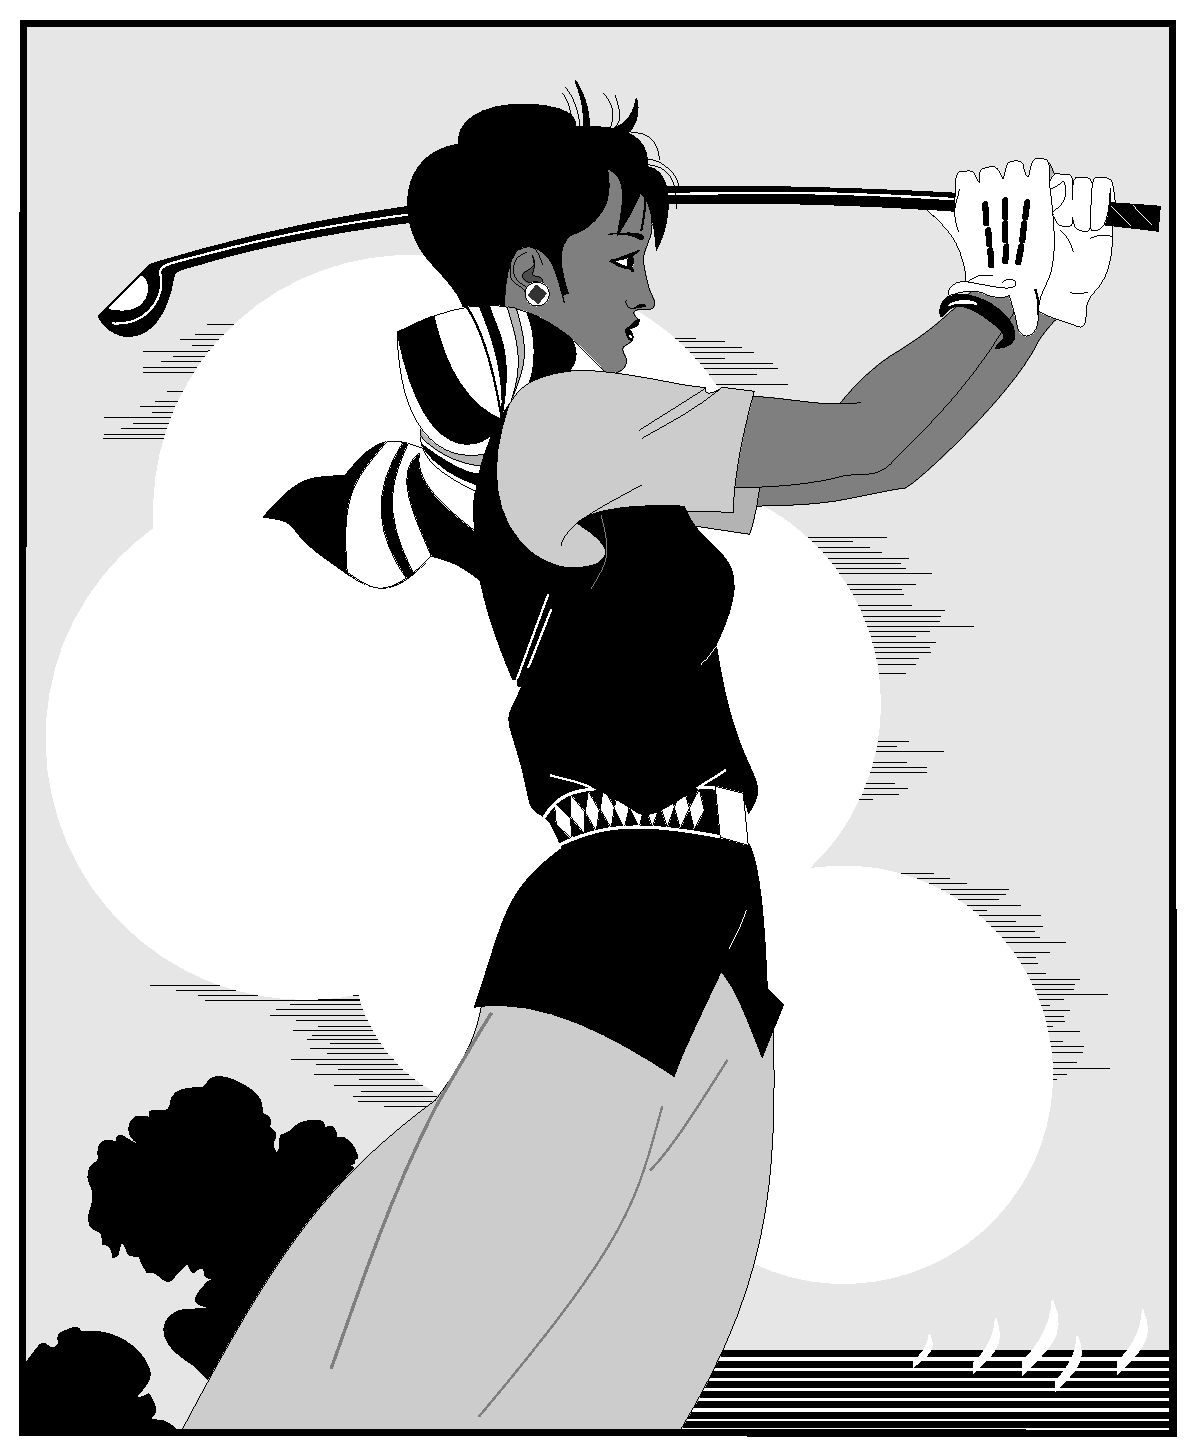
\includegraphics[width = 0.4\textwidth]{golfer}
\FigureBiCaption{��߶��������}{Golfer}
\label{Figure:Tricks:Example1}
\end{figure}

���ijͼ��ܳ��Ļ�������ͨ���ֲ��ı�\verb|\captionwidth|�Ŀ��Ƚ��ж��С�
ͼ~\ref{Figure:Tricks:Example11}������һ����Ӣ�ı�����������ӡ�

\begin{figure}[htbp]
\centering
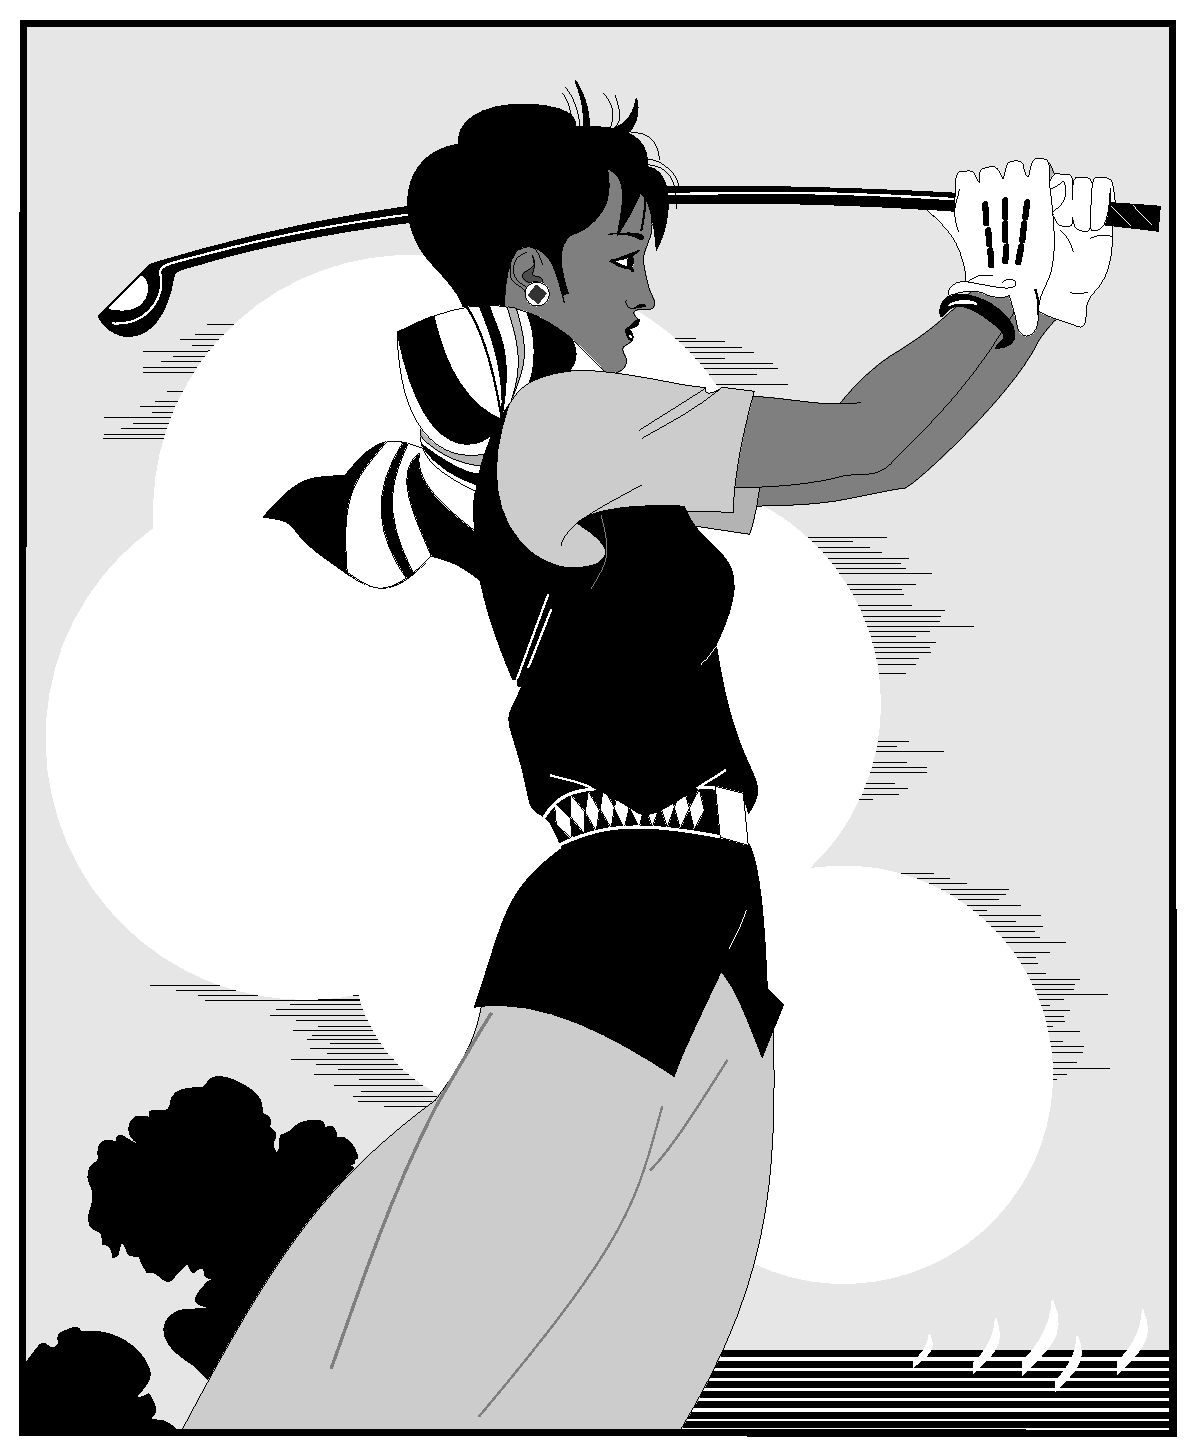
\includegraphics[width = 0.4\textwidth]{golfer}
\changecaptionwidth \captionwidth{0.7\textwidth}
\FigureBiCaption{һ����߶�������˴� �߶�������˴�߶���
�߶�������� ��߶� ������˴�߶����� ���˴�߶������
�˴�߶��������}{Golfer Golfer This is a very good idea and i
like it very much do u like it Golfer Golfer Golfer Golfer Golfer
Golfer Golfer Golfer Golfer} \label{Figure:Tricks:Example11}
\end{figure}

\normalcaptionwidth
ͼ~\ref{Figure:Tricks:Example12}�ǻָ�Ĭ�Ͽ���֮���ͼ�����ӡ�
\begin{figure}[htbp]
\centering
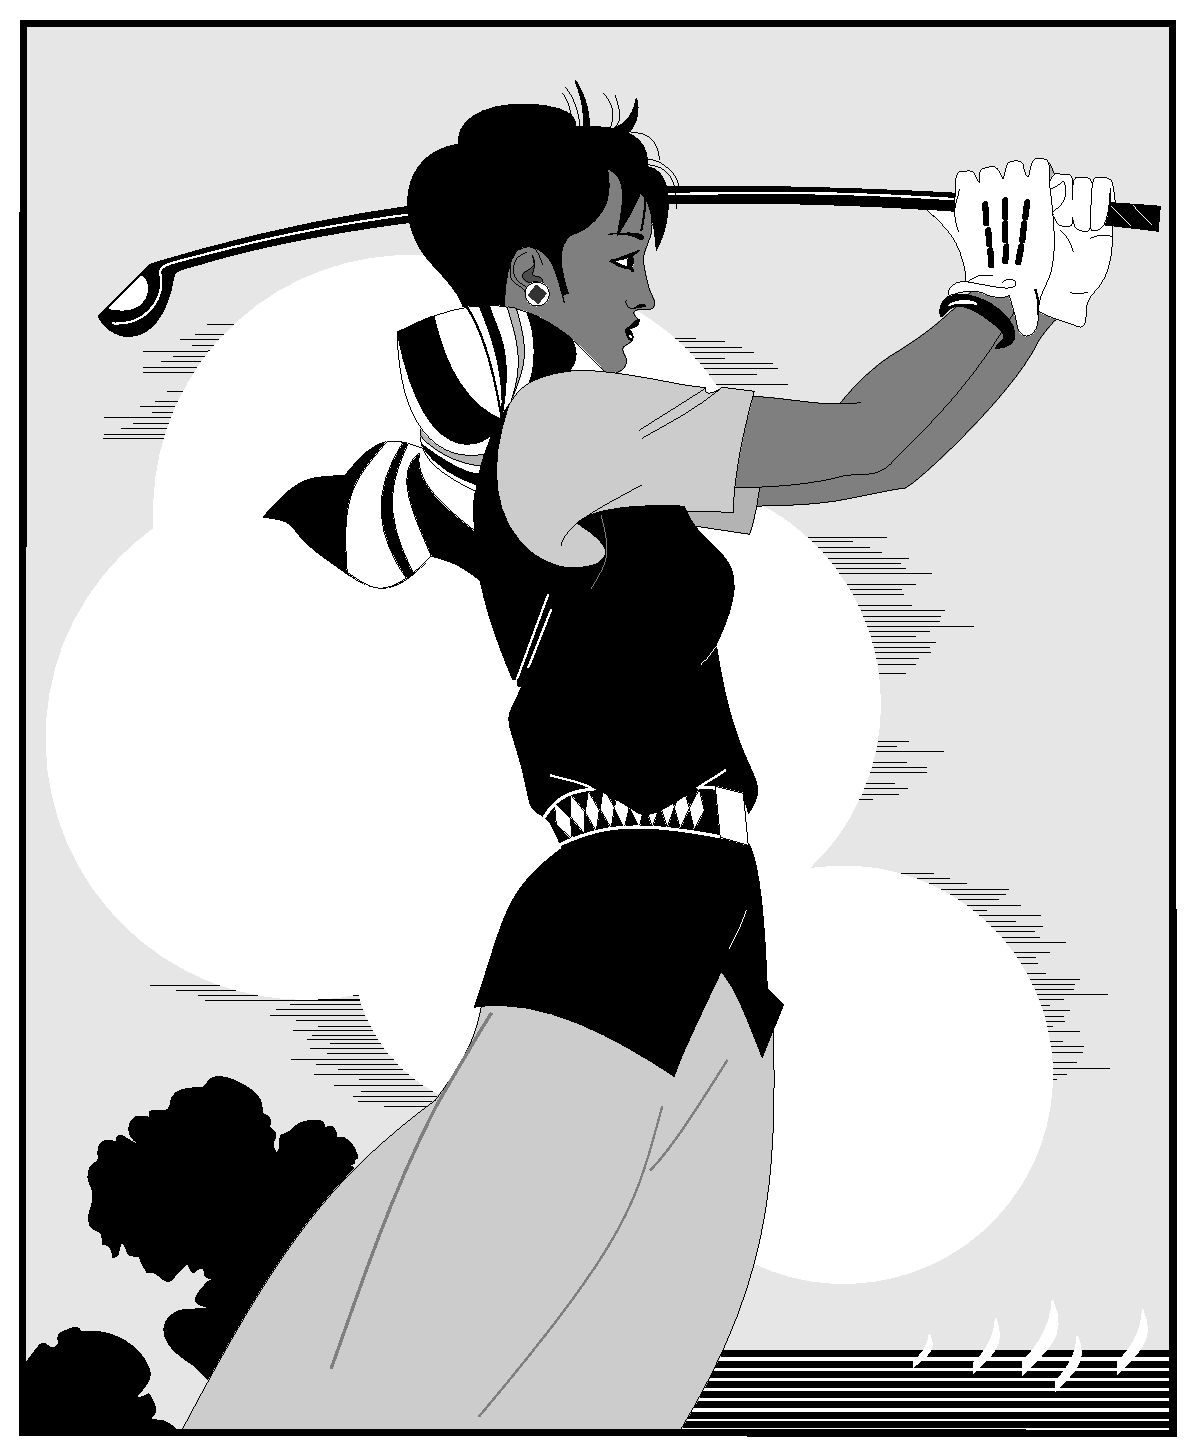
\includegraphics[width = 0.4\textwidth]{golfer}
\FigureBiCaption{��߶�������˴�߶�������˴�߶���߶�������˴�߶�������˴�߶�������˴�߶�������˴�߶��������}{Golfer Golfer Golfer Golfer Golfer Golfer   Golfer Golfer Golfer Golfer Golfer Golfer Golfer Golfer Golfer Golfer Golfer Golfer}
\label{Figure:Tricks:Example12}
\end{figure}


Ϊ��ͼ������һ��Ӣ�ı������
\begin{verb}
\SubfigEnCaption{Ӣ��}��
\end{verb}
�ڽ�����~subfigure~�������������,������Ӣ�ı��⡣
��һ�в�ֻһ����ͼʱ,��ͼ����~minipage~�У���~minipage~����������

ͼ~\ref{Figure:Tricks:Example2} ������һ��ֻ��һ����ͼ�����ӡ�

ͼ~\ref{Figure:Tricks:Example3} ������һ���ж����ͼ�����ӡ�
\begin{figure}[htbp]
\centering
\subfigure[�߶���]{\label{Figure:Tricks:Example2:a}
  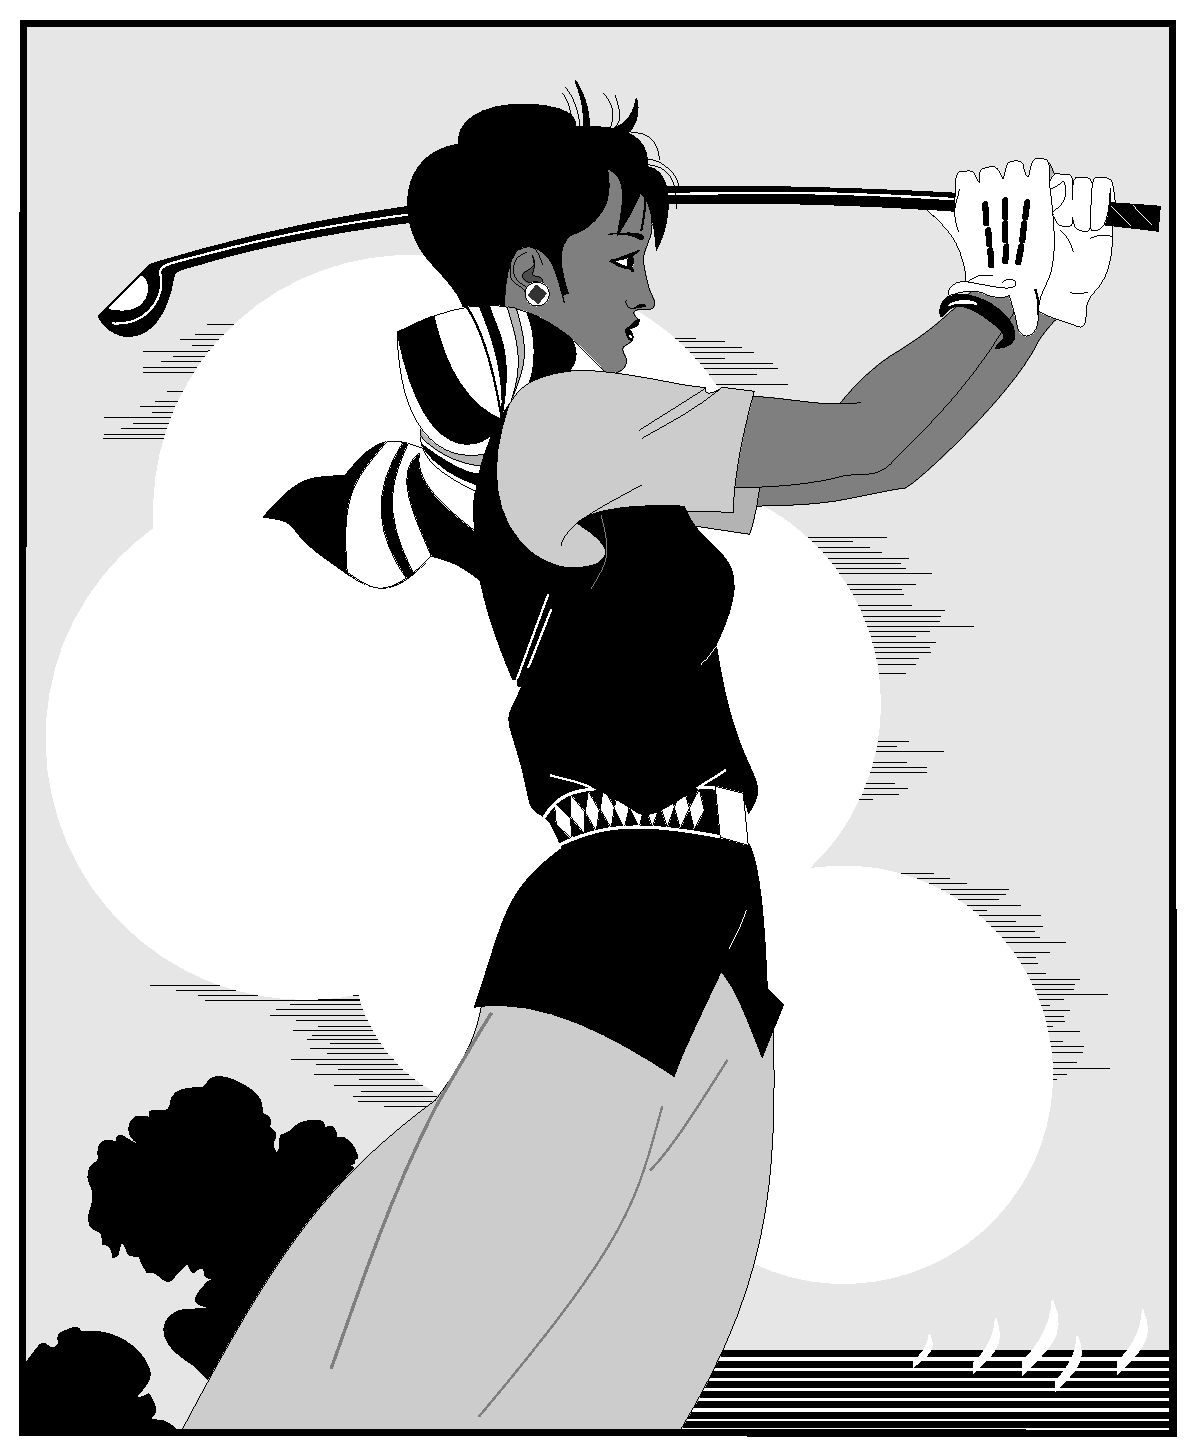
\includegraphics[width = 0.22\textwidth]{golfer}
}\SubfigEnCaption{Golfer1}
\subfigure[�߶���]{\label{Figure:Tricks:Example2:B}
  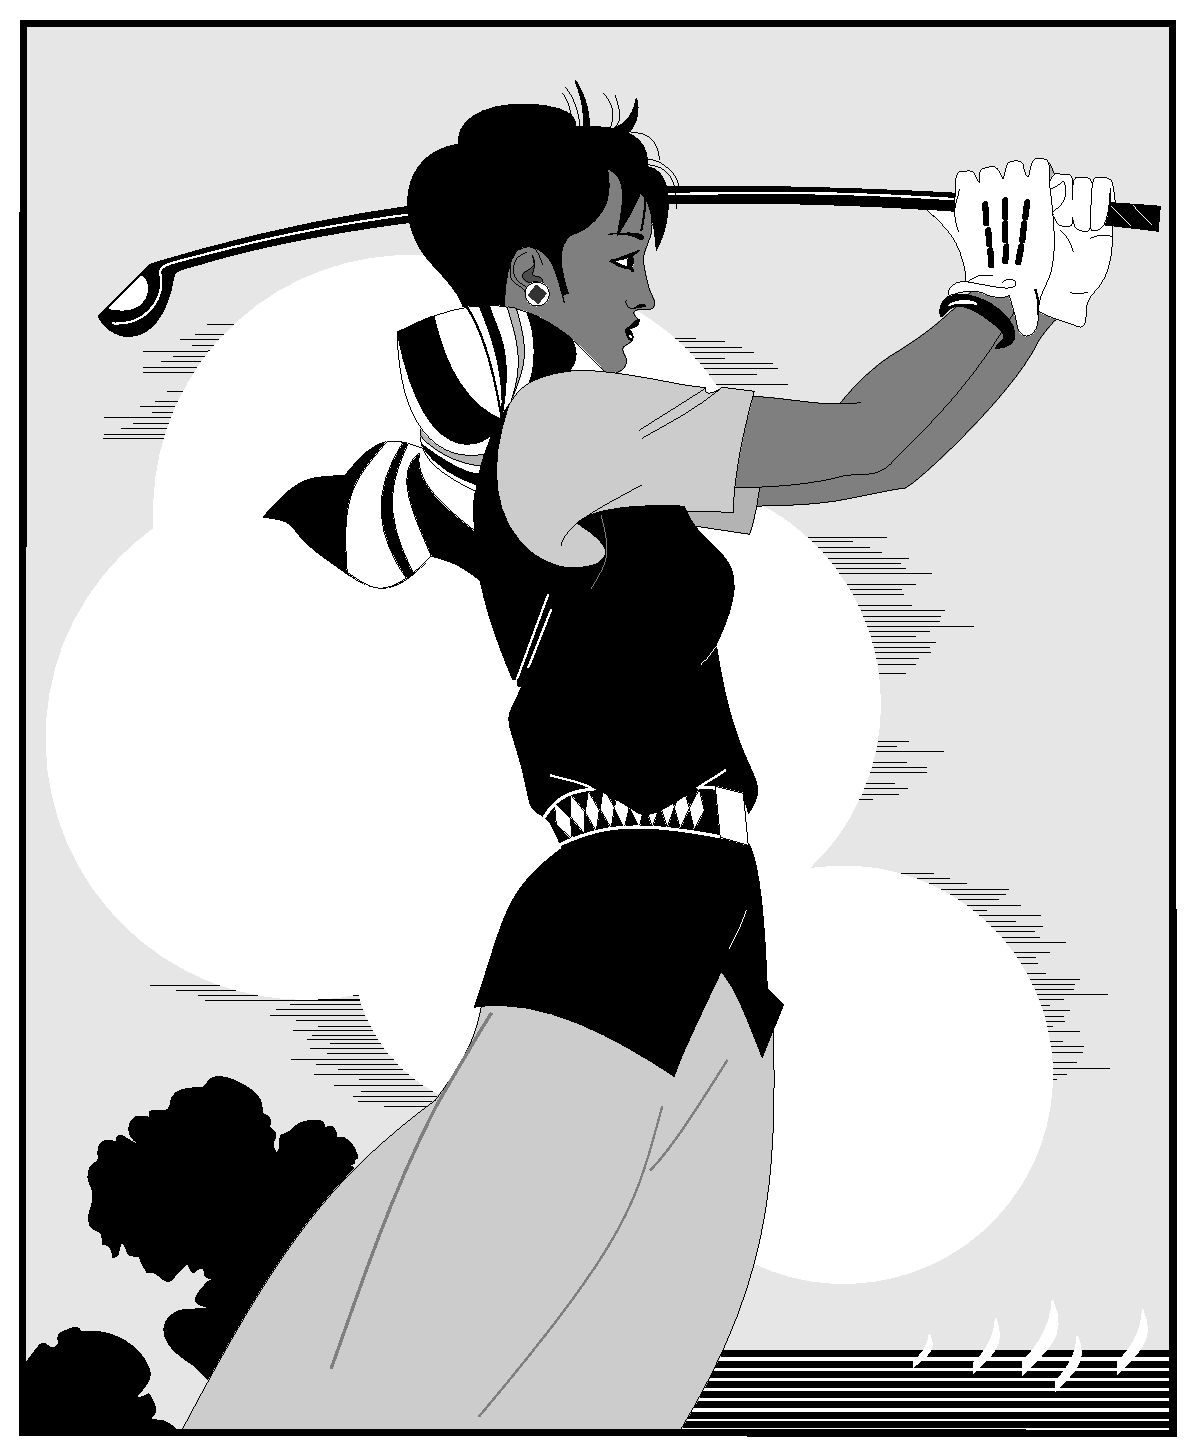
\includegraphics[width = 0.22\textwidth]{golfer}
}\SubfigEnCaption{$I_{\rm dc} = 0.5 III$A}
\FigureBiCaption{�߶���}{Golf}
\label{Figure:Tricks:Example2}
\end{figure}

\begin{figure}[htbp]
\centering
\begin{minipage}{0.25\textwidth}
\centering
\subfigure[�߶���]{\label{Figure:Tricks:Example3:a}
  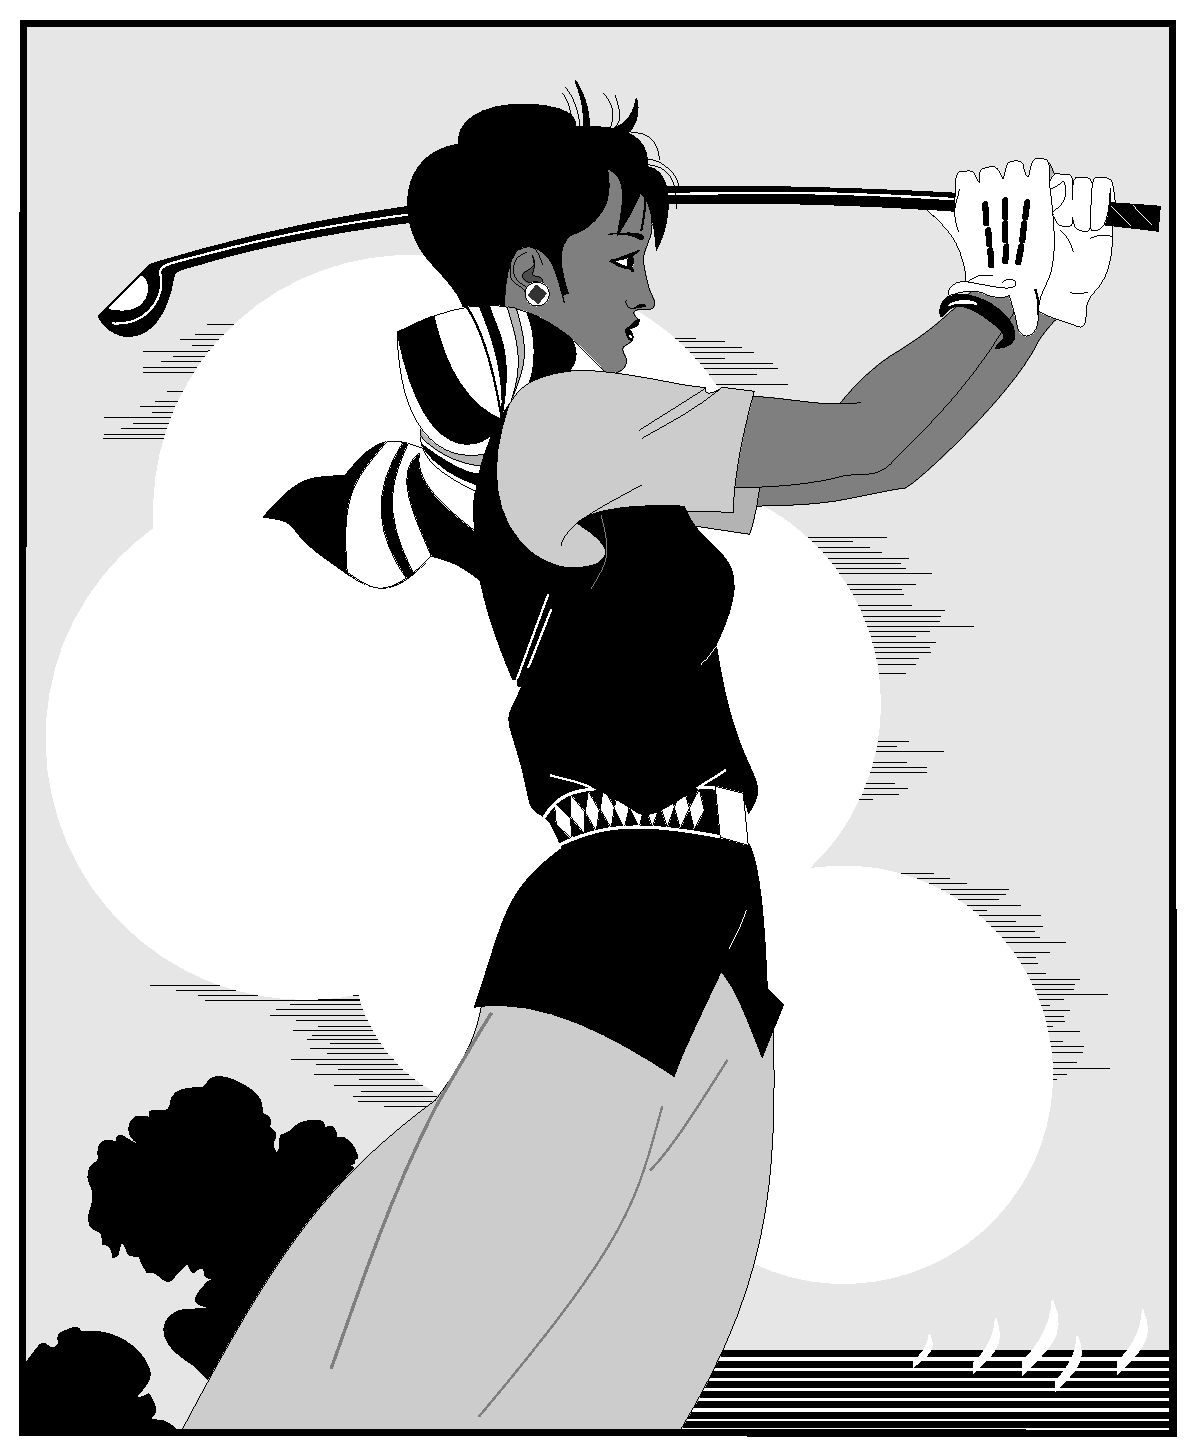
\includegraphics[width = \textwidth]{golfer}
}\vspace*{-5pt}\SubfigEnCaption{Golfer1}
\end{minipage}
\begin{minipage}{0.25\textwidth}
\centering
\subfigure[�߶���]{\label{Figure:Tricks:Example3:B}
  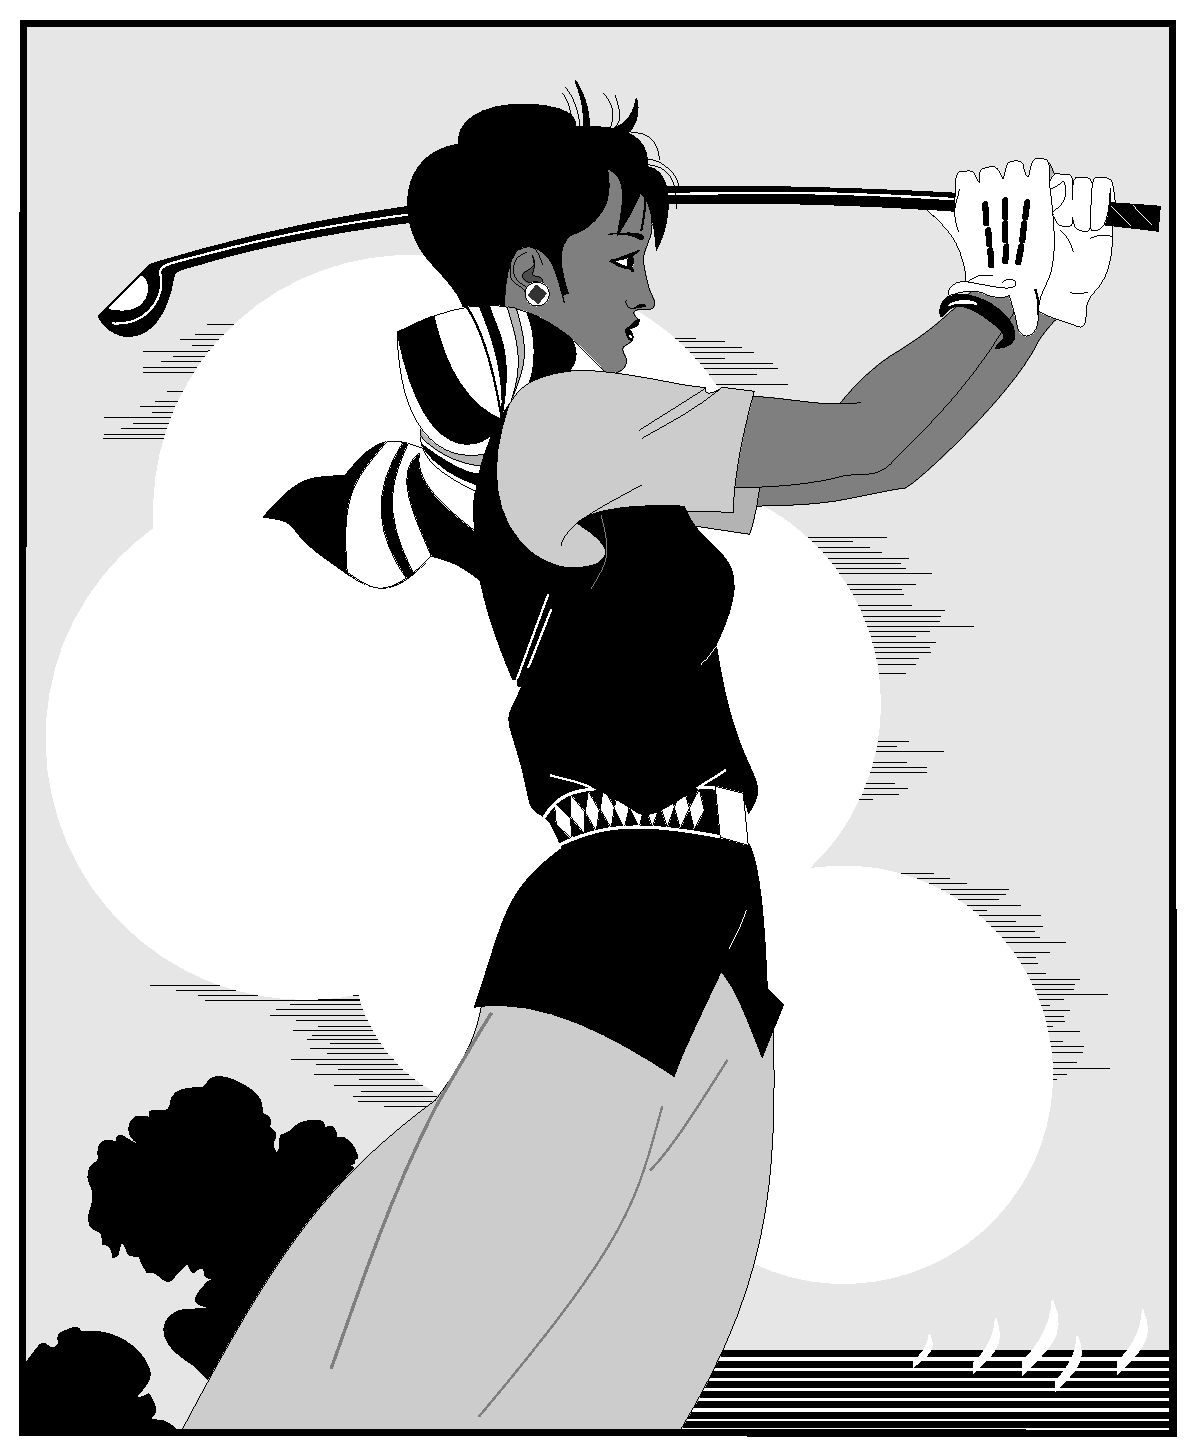
\includegraphics[width = \textwidth]{golfer}
}\vspace*{-5pt}\SubfigEnCaption{Golfer2}
\end{minipage}
\begin{minipage}{0.25\textwidth}
\centering
\subfigure[�߶���3]{\label{Figure:Tricks:Example3:C}
  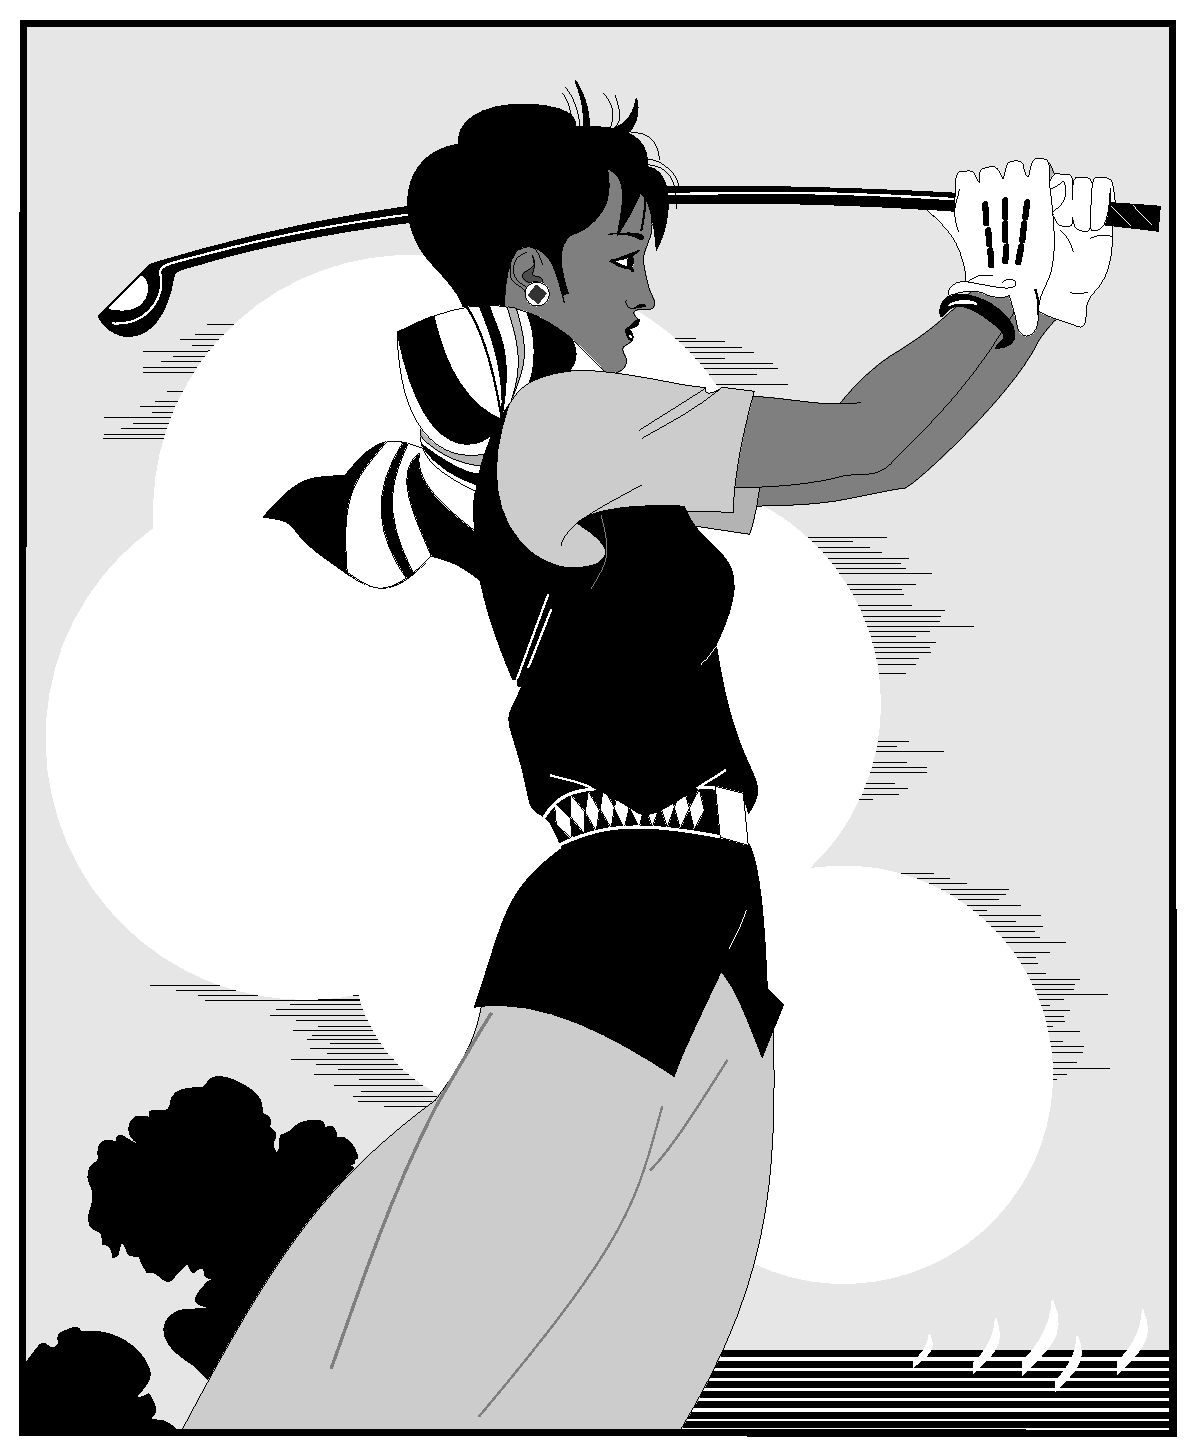
\includegraphics[width = \textwidth]{golfer}
}\vspace*{-5pt}\SubfigEnCaption{Golfer3}
\end{minipage}
\FigureBiCaption{�߶���}{Golf}
\label{Figure:Tricks:Example3}
\end{figure}

ͼ~\ref{Figure:Tricks:Example31} ������һ����ͼͼ�����������
\begin{figure}[htbp]
\centering
\begin{minipage}[t]{0.20\textwidth}
\centering
\subfigure[�߶���߶���߶���߶���]{\label{Figure:Tricks:Example31:a}
  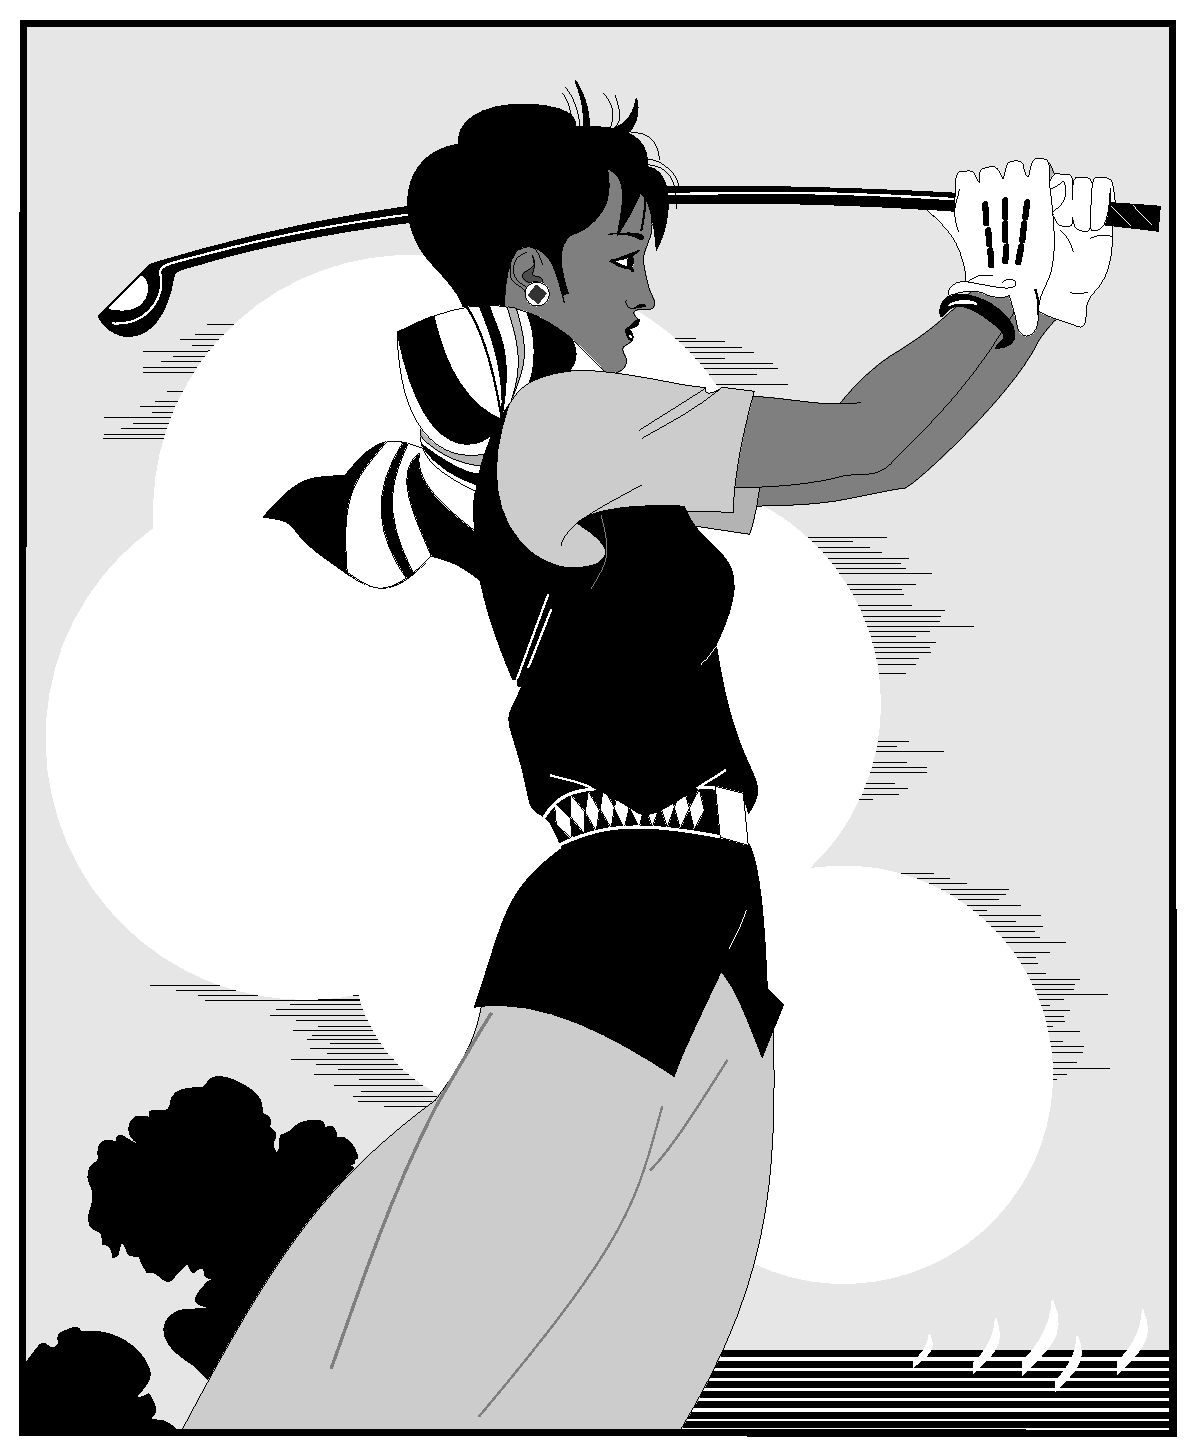
\includegraphics[width = \textwidth]{golfer}
}\SubfigEnCaption{Golfer1 Golfer1 Golfer1 Golfer1 Golfer1}
\end{minipage}\hspace{2em}
\begin{minipage}[t]{0.20\textwidth}
\centering
\subfigure[�߶���߶���߶���߷�]{\label{Figure:Tricks:Example31:B}
  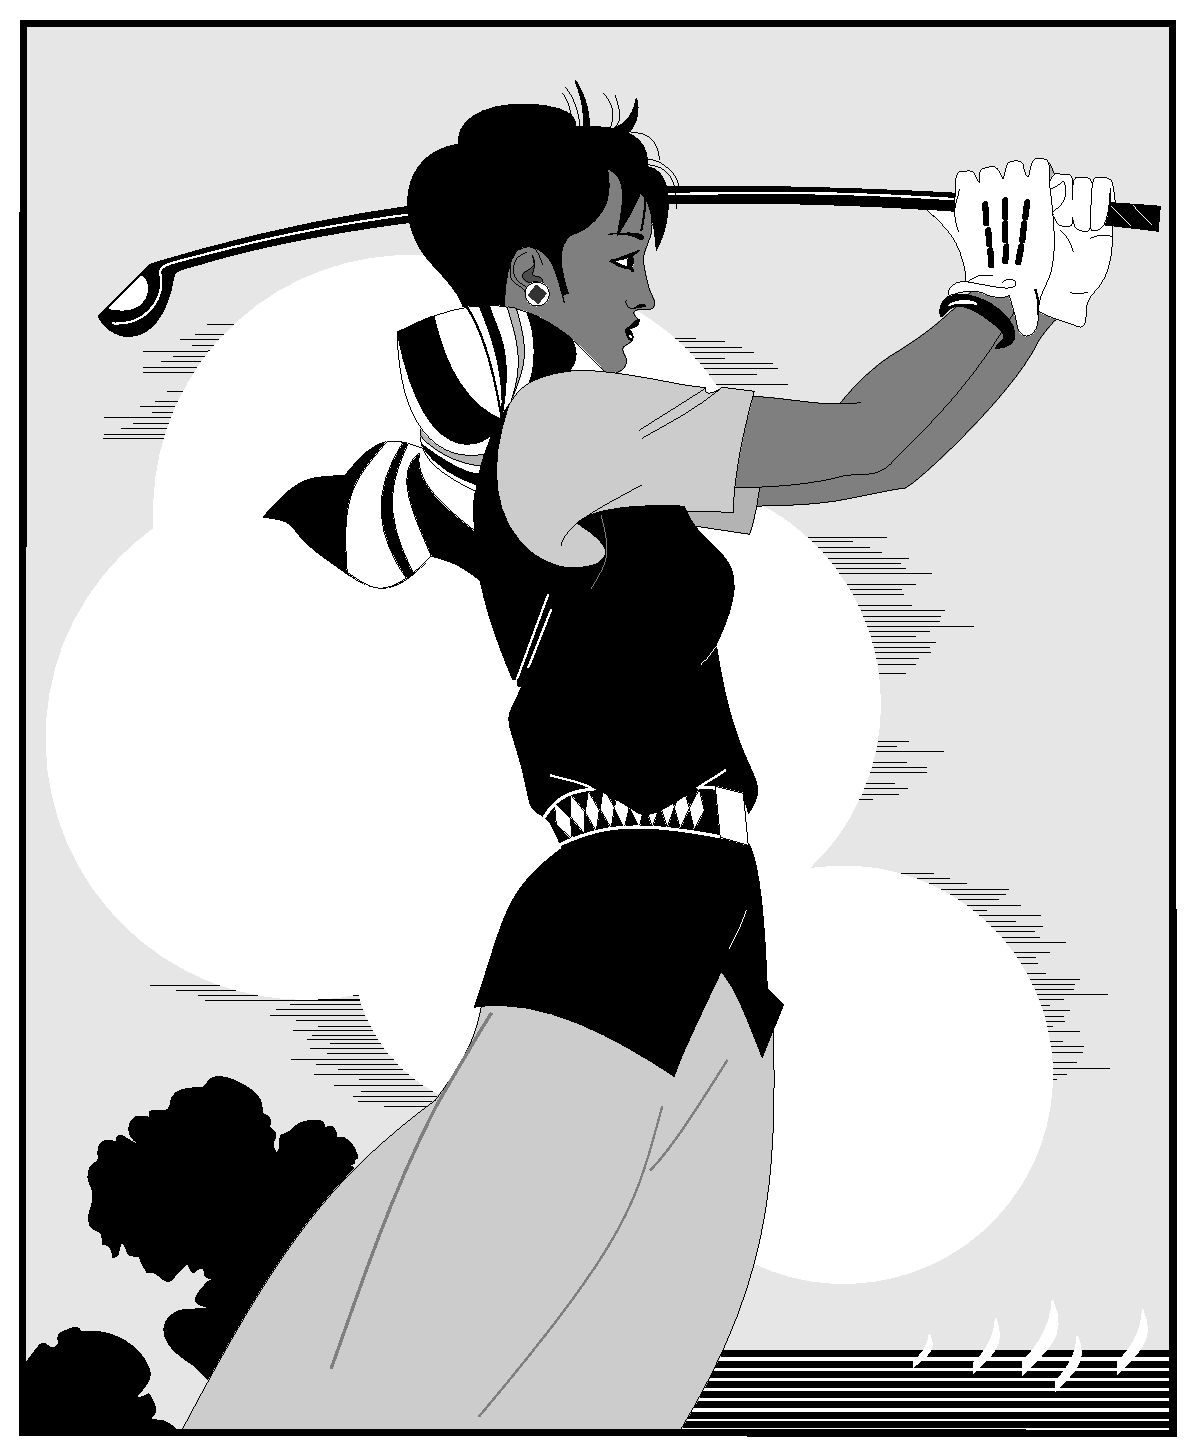
\includegraphics[width = \textwidth]{golfer}
}\SubfigEnCaption{G G f f f f f f f f f f f f f f f f f f}
\end{minipage}\hspace{2em}
\begin{minipage}[t]{0.20\textwidth}
\centering
\subfigure[�߶���߶���߶���߶�3]{\label{Figure:Tricks:Example31:C}
  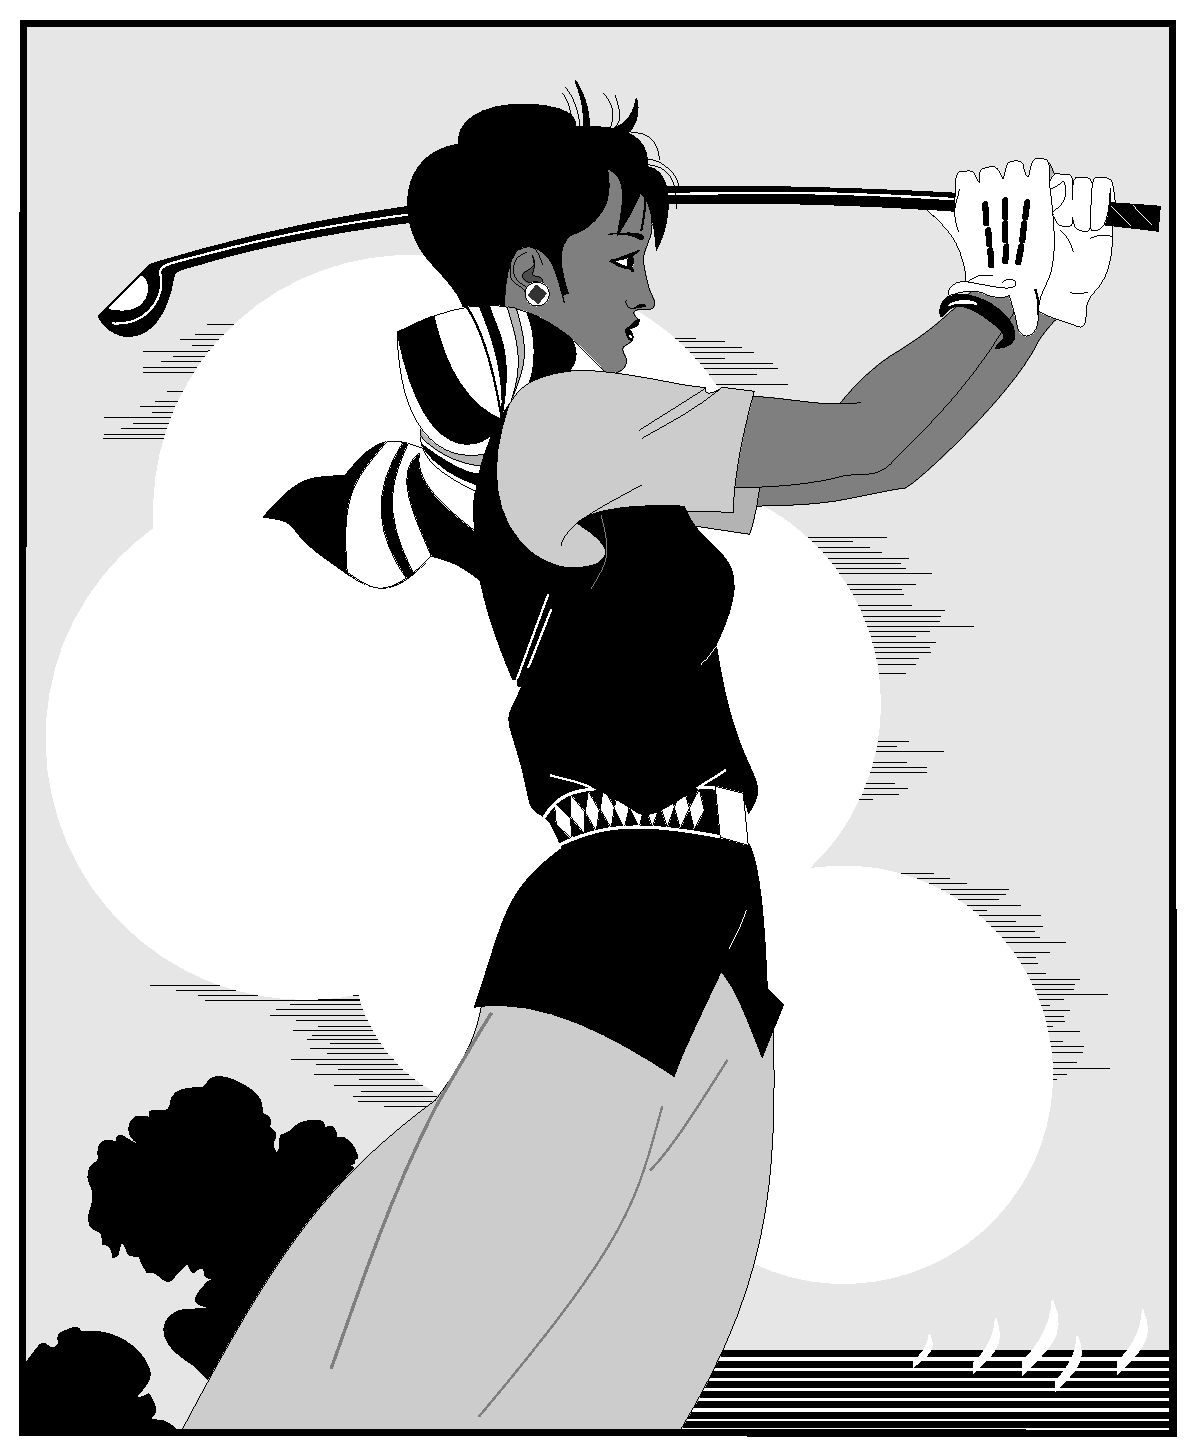
\includegraphics[width = \textwidth]{golfer}
}\SubfigEnCaption{Golfer3 Golfer3 Golfer3 Golfer3 Golfer3 Golfer3}
\end{minipage}
\FigureBiCaption{��ͼ���߶��� �߶��� �߶��� �߶��� �߶���}{Parent: Golf Golf Golf Golf Golf}
\label{Figure:Tricks:Example31}
\end{figure}


\BiSubsection{������}{Caption of Tables}
ģ���зֱ�Ϊ��������˫�������
\verb"\TableBiCaption{����}{Ӣ��}"��
�������������������һ��Ϊ���ı��⣬�ڶ���ΪӢ�ı��⣬Ч����~\ref{Tricks:Tab1}��


\begin{table}[htbp]
\centering 
\TableBiCaption{�������}{Test of Table}
\label{Tricks:Tab1}
\begin{tabular}{c|c|c}
  \hline
  % after \\: \hline or \cline{col1-col2} \cline{col3-col4} ...
  ���� & ����~(\%) & �ٶ�~(ms) \\
  \hline
  С���任 & $99.8$ &  20\\
  ����Ҷ�任 & $99.0$ & 30 \\
  \hline
\end{tabular}
\end{table}

���ڳ��������Ӣ�ı��⣬����~\verb"\LTBiTocCaption{���ij����̱��⣨Ŀ¼�У�}{���ij��������⣨�����У�}{Table}{Ӣ�ij����̱��⣨Ŀ¼�У�}{Ӣ�ij��������⣨���ģ�}"
~�����塣��Ҫע����ǣ�����������~\verb|ccaption| ����еij�������⴦����ʽ������5��������
��������������ı䣬���������������ƣ����������׼��٣�������˶��塣
����������������ı��������ĺ�ͼ��Ŀ¼���������Ű棬���Һ���������ı��Э����
�����Ҫ���ó�������~\verb|\LTBiTocCaption|����֮�����~\verb|\label| ���
��~\ref{table:LTexample} ����һ�����ӡ�

\begin{longtable}{lll} 
\LTBiTocCaption{���ı����}{���ı��ⳤ}{Table}{Long Table  Short Caption}{Long Table Long Caption}\label{table:LTexample}\\
\bfseries Entity & \bfseries Unicode Name & \bfseries Unicode \\ \hline
\endfirsthead
\bfseries Entity & \bfseries Unicode Name & \bfseries Unicode \\ \hline
\endhead
\hline \multicolumn{3}{r}{\emph{Continued on next page}}
\endfoot
\hline
\endlastfoot
a&bcd&bcdef\\
����&��������&����\\
a&emf&bcdef\\
a&emf&bcdef\\
a&emf&bcdef\\
a&emf&bcdef\\
a&emf&bcdef\\
a&emf&bcdef\\
a&emf&bcdef\\
a&emf&bcdef\\
a&emf&bcdef\\
a&emf&bcdef\\
a&emf&bcdef\\
a&emf&bcdef\\
a&emf&bcdef\\
a&emf&bcdef\\
a&emf&bcdef\\
a&emf&bcdef\\
a&emf&bcdef\\
a&emf&bcdef\\
%a&emf&bcdef\\
\end{longtable}

%\iffalse

\BiSection{�㷨}{algorithm}
����һ���㷨�����ӣ�����~worldguy@lilacbbs~
\begin{algorithm}
\KwIn{training samples, {$(d_i, d_j)_q$; $\mathbf{q}_i, \mathbf{q}_j \in C$,
$q\in \mathbf{Q}$} }
\KwOut{parameter setting $\lambda^T$}

\For{$t$=1 to $T$}
{   
    $\lambda^{t+1}_n = \lambda^t_n + \eta (f_n(q, c, d_i) - f_n(q, c, d_j))$
 }
\end{algorithm}
�㷨�������Ҳ�հױȽ϶࣬������Ҳ�Ŀհ׿��С�����Բ���minipage����ʵ�֡���algorithm�����ŵ�minipage�������棬���Ҽ���ѡ��[H]��ֹ�㷨�������������һ�����ӡ���Ҫ˵�����ǣ�һ�㲻��Ҫ�������ִ������㷨������п��ޣ����б���Ļ�����ʹ��\verb|\caption|����������Ӣ��˫���⣬�����Ҳο�ͼ�������Լ�����һ�¡�

\begin{minipage}{0.8\textwidth}
\vspace{5mm}
\begin{algorithm}[H]
\caption{����һ���㷨����}
\KwIn{training samples, {$(d_i, d_j)_q$; $\mathbf{q}_i, \mathbf{q}_j \in C$,
$q\in \mathbf{Q}$} }
\KwOut{parameter setting $\lambda^T$}

\For{$t$=1 to $T$}
{   
    $\lambda^{t+1}_n = \lambda^t_n + \eta (f_n(q, c, d_i) - f_n(q, c, d_j))$
 }
\end{algorithm}
\end{minipage}


\BiSection{��ʽ}{Equations}
\label{Tricks:Equations}

�ı��е���ѧ���ź͹�ʽ������ķ������룺

������ѧ��������ȡ��һ���������ģ�;���ͨ����˵��$N$�����⣬����һ
�������£����о������屻�����ʵ㣬$N$��������򵥵ľ��Ƕ������⡣��һ
������ϵͳ�У�$N$��������������$n$���������$k$��С����($N=n+k$)������
$k$��С�������$n$�����������С���Ժ����˶���Ӱ�켸�����ÿ��ǣ���$k$
��С����֮��������Ͻ�������֮����໥����Ӧ�迼�ǣ���͹���������
��($n+k$)�����⡣�ر�أ���$N=3,~n=2,~k=1$ʱ����ͨ����˵���������������⡣


���������ѧ��ʽ������ŵģ�
\begin{equation}
\ddot{\mathbf{r}}=\mathbf{F}_{0}(r)+\mathbf{F}_{\varepsilon}(\mathbf{r},\dot{\mathbf{r}},t)
\end{equation}
\eqref{eq:noindex}��һ��������ŵ����ӣ�
\begin{displaymath}\label{eq:noindex}
F_{\varepsilon}/F_{0}=O (\varepsilon)
\end{displaymath}

\FloatBarrier %���������
���͵Ĺ�ʽ�ӷ���˵�������ӣ�

ʽ\eqref{eq:1}ΪĿ���������׷�ٷ�����֮�������˶�����
\begin{equation}\label{eq:1}
\ddot{\boldsymbol{\rho}}-\frac{\mu}{R_{t}^{3}}\left( 3\mathbf{R_{t}}\frac{\mathbf{R_{t}\rho}}{R_{t}^{2}}-\boldsymbol{\rho}\right)=\mathbf{a}
\end{equation}
����

$\boldsymbol{\rho}$---׷�ٷ�������Ŀ�������֮������λ��ʸ����

$\ddot{\boldsymbol{\rho}}$---׷�ٷ�������Ŀ�������֮�����Լ��ٶȣ�

$\mathbf{a}$---�����������ļ��ٶȣ�

$\mathbf{R}_{t}$---Ŀ��������ڹ�������ϵ�е�λ��ʸ����

$\omega_{t}$---Ŀ��������Ĺ�����ٶȣ�

$\mathbf{g}$---�������ٶȣ�$=\frac{\mu}{R_{t}^{3}}\left(
3\mathbf{R_{t}}\frac{\mathbf{R_{t}\rho}}{R_{t}^{2}}-\boldsymbol{\rho}\right)=\omega_{t}^{2}\frac{R_{t}}{p}\left(
3\mathbf{R_{t}}\frac{\mathbf{R_{t}\rho}}{R_{t}^{2}}-\boldsymbol{\rho}\right)$������$p$��Ŀ��������Ĺ����ͨ����

��ʽ�ӷ���˵��������������
\begin{equation}\label{eq:111}
\ddot{\boldsymbol{\rho}}-\frac{\mu}{R_{t}^{3}}\left( 3\mathbf{R_{t}}\frac{\mathbf{R_{t}\rho}}{R_{t}^{2}}-\boldsymbol{\rho}\right)=\mathbf{a}
\end{equation}
\begin{formulasymb}{ʽ��}{-15pt}%-3pt,-20pt�����Ϸ��ļ�ࡣ
  \fdesfirst{$\boldsymbol{\rho}$}{׷�ٷ�������Ŀ�������֮������λ��ʸ����}
  \fdes{$\ddot{\boldsymbol{\rho}}$}{׷�ٷ�������Ŀ�������֮�����Լ��ٶȣ�}
  \fdes{$\mathbf{a}$}{�����������ļ��ٶȣ�}
  \fdes{$\mathbf{R}_{t}$}{Ŀ��������ڹ�������ϵ�е�λ��ʸ����}
  \fdes{$\omega_{t}$}{Ŀ��������Ĺ�����ٶȣ�}
  \fdes{$\mathbf{g}$}{�������ٶȣ�$=\frac{\mu}{R_{t}^{3}}\left(
3\mathbf{R_{t}}\frac{\mathbf{R_{t}\rho}}{R_{t}^{2}}-\boldsymbol{\rho}\right)=\omega_{t}^{2}\frac{R_{t}}{p}\left(
3\mathbf{R_{t}}\frac{\mathbf{R_{t}\rho}}{R_{t}^{2}}-\boldsymbol{\rho}\right)$������$p$��Ŀ��������Ĺ����ͨ����}
\end{formulasymb}

���о�����������Ĺ�ʽ��
\begin{equation}\label{eq:rho}
\dot{\boldsymbol{\rho}}=\left( \begin{array}{c}
\dot{x}-\omega_{t}y\\\dot{y}+\omega_{t}x\\\dot{z}
\end{array}\right) , \quad
\ddot{\boldsymbol{\rho}}=\left( \begin{array}{c}
\ddot{x}-2\omega_{t}\dot{y}-\omega_{t}^{2}x-\dot{\omega}_{t}y\\
\ddot{y}+2\omega_{t}\dot{x}-\omega_{t}^{2}y+\dot{\omega}_{t}x\\
\ddot{z}
\end{array}\right)
\end{equation}

���ڷֿ���󣬿��Բ���~arydshln~�������ģ�����Ѿ�������һ�����֧�֣�ʹ��ʱ������������ոú���Դ����ĵ���
\begin{equation}
A = \left\{ \begin{array}{cc:c} %: ��ʾ�������ߣ�
 x & y & z \\
 u & v & w \\ \hdashline   %�������
 x & y & z
 \end{array} \right\}
 \end{equation}


����һЩ�ϳ���ʽ��һ��д���£��������У�
{\setlength\arraycolsep{2pt}
\begin{eqnarray}
x & = & \left( x_{0}+\frac{2\dot{y}_{0}}{\omega_{t}}+\frac{4a_{x}}{\omega_{t}^{2}}\right) +2\left( \frac{2\dot{x}_{0}}{\omega_{t}}-3y_{0}-\frac{a_{y}}{\omega_{t}^{2}}\right) \sin (\omega_{t} t)- \nonumber\\
& & 2\left( \frac{\dot{y}_{0}}{\omega_{t}}+\frac{2a_{x}}{\omega_{t}^{2}}\right) \cos (\omega_{t} t)-\left( 3\dot{x}_{0}-6\omega_{t} y_{0}-\frac{2a_{y}}{\omega_{t}}\right) t-\frac{3a_{x}}{2}t^{2} \\
y & = & \left( 4y_{0}-\frac{2\dot{x}_{0}}{\omega_{t}}+\frac{a_{y}}{\omega_{t}^{2}} \right) +\left( \frac{\dot{y}_{0}}{\omega_{t}}+\frac{2a_{x}}{\omega_{t}^{2}}\right) \sin (\omega_{t} t) -\nonumber\\
& & \left( 3y_{0}-\frac{2\dot{x}_{0}}{\omega_{t}}+\frac{a_{y}}{\omega_{t}^{2}}\right) \cos (\omega_{t}t)-\frac{2a_{x}}{\omega_{t}}t \\
z & = & \frac{\dot{z}_{0}}{\omega_{t}}\sin (\omega_{t}t)+\left( z_{0}-\frac{a_{x}}{\omega_{t}^{2}}\right)\cos (\omega_{t}t)+\frac{a_{z}}{\omega_{t}^{2}}
\end{eqnarray}}
���ʵ��û�а취�Ͽ���������~relsize~����е�~mathsmaller mathlarger �����������壬�ﵽ���ŵ�Ŀ�ģ�mathsmaller ������Է����ö�Ρ�

�������������ʽʱ����Ҫÿ����ʽ����~equation~������������ʹ�ù�ʽ֮��ľ���ܴ�
�Ƽ�ʹ��~align��gather��eqnarray �Ȼ�����
�����뿴\href{ftp://ftp.ctex.org/pub/tex/documents/bible/LaTeX_Companion_ch8.zip}{The LaTeX Companion �ĵ�8��}��
ǰ���Ѿ����������㰲װ����CTeX��װ�Ѿ����д��ĵ���

��������£���Ҫ��ʽ��ʱ����룬��ʱ����Բ���ģ���Զ����~flualign~������ʵ�֡�Ч�����£�
\begin{flualign}
a=\delta
\end{flualign}

����ͨ��~\verb"\setlength\jot{����}"~���趨��ʽ֮��ľ��룬Ĭ��Ϊ~3pt����ģ�彫���趨Ϊ~8pt��
\begin{gather}
\alpha + \beta = \gamma\\
x^2+y^2=z^2\\
E=mc^2
\end{gather}

\BiSection{һ������С�ڱ���һ������С�ڱ���һ������С�ڱ���һ������С�ڱ���һ������С�ڱ���һ������С�ڱ���}{A Long Section Title Example}\label{tricks:Longsectiontitle}

��\ref{tricks:Longsectiontitle}��һ���ڱ�����������ӡ��±������������Ҳ�Ѿ��������������±������ʱ�ֶ����еĴ��롣
\begin{verbatim}\BiChapter[����±���̫���ˣ���Ҫ������ô��]{����±���̫����,\\��Ҫ������ô��}
{the chapter title is too long}\end{verbatim}

\BiSection{ģ�����Զ����һЩ����}{Some Commands Defined in the Template}
�������ģ�����Զ����һЩ�����Ҫ���ܣ���ϸ�÷��ɲ���ģ���е�ʾ���ļ�~Tricks.tex �ȡ�
\begin{hitlist}
\item \verb+\citeup+~����~\verb+\ucite+���������ϱ���ʽ���òο����ף�\verb+\cite+�������÷�ʽ
\item ˫���½����\verb+\BiChapter, \BiSection, \BiSubsection+\\
\verb+\BiSubsubsection, \BiAppChapter, \BiAppendixChapter+
\item ˫��ͼ�����\verb+\FigureBiCaption, \SubfigEnCaption+\\
\verb+\TableBiCaption, \LTBiTocCaption+
\item ������1����ʽ����~formulasymb��2������빫ʽ~flualign��3���б�����~hitlist��~publist 
\item �������ۺ�~\verb+\cdash+����ѧģʽ������΢��~dx~\verb+\dif+��
\item �����ֺ��������\verb+\normalbiao+��\verb+\wuhaobiao+
\item �ֺ����\verb+\yihao, \erhao, \xiaoer, \sanhao, \xiaosan+\\
\verb+\sihao, \xiaosi, \wuhao, \xiaowu+������Ĭ����������~\verb+defaultfont+
\end{hitlist}


\BiSection{Pluto~ģ��~FAQs}{FAQs of the PlutoThesis template}
\noindent \textbf{Q1}��\textcolor{blue}{�������������һ�Σ��������ð���}\\
\textbf{A1}�������о���Ժ���ġ����Ĺ淶��������������ǽ���д�����������������������һ�Ρ������Ҫ��
������~format.tex ��Ѱ�����´��룺
\begin{verbatim}
  \titleformat{\subsubsection}[runin]{\hei\sf\xiaosi}
  {\thesubsubsection}{0.5em}{}[\;\;]
\end{verbatim}
����
\begin{verbatim}
  \titleformat{\subsubsection}[hang]{\hei\sf\xiaosi}
  {\thesubsubsection}{0.5em}{}
\end{verbatim}

\noindent \textbf{Q2}��\textcolor{blue}{ͼ�����ͼ��֮�������ô�������о��е��}\\
\textbf{A2}���ֶ��ɣ�\verb+\vspace*{-8pt}\FigureBiCaption+

\noindent \textbf{Q3}��\textcolor{blue}{�ο������б���Ĵ�Сд�����⣬����д�Ĵ�д����ôת��Сд�ˣ�}\\
\textbf{A3}���ο����׵ı����ʵ������ĸ�Զ���д��������ĸСд������һЩ����ʣ����磺
\verb+{IEEEtran \LaTeX}+ Ӧ��д�� \verb+{IEEEtran} {\LaTeX}+��$\lambda$ Ӧ��д��
\verb+{$\lambda$}+��BaTiO3~дΪ\verb+{BaTiO3}+��

\noindent \textbf{Q4}��\textcolor{blue}{��ͼ������~[~��~]~����ʱ�����dz���ѽ}\\
\textbf{A4}������~subfigure~ʱ�������ͼ���⺬��~[~����Ҫ��~\{~��~\}~��Χ������
\verb+$\beta\in{[0,\,\pi]}$+

\noindent \textbf{Q5}��\textcolor{blue}{���ʱ����еĶ��˺͵Ͷ˵�"����"��ô��}\\
\textbf{A5}��ԭ������\verb+\hline+�ĵط���������\verb+\toprule+��������\verb+\bottomrule+��
����\verb+\specialrule{1pt}{0pt}{0pt}+��

\noindent \textbf{Q6}��\textcolor{blue}{��ôͳ�����ĵ�������}\\
\textbf{A6}��һ����������ַ������Թ���������1. dos������ charcnt main.dvi������~$\approx$~ȫ���ַ���~+~�����ַ���/5��
2. ��~.pdf ����Ϊ~.rtf �ļ���Ȼ����~MS Word~��������ͳ�ơ�

\noindent \textbf{Q7}��\textcolor{blue}{���µ�ͼ�������ڲ�ͬ�����ļ�����?}\\
\textbf{A7}��\verb+\graphicspath{{figures/chp1/}{figures/chp2/}}+��

\noindent \textbf{Q8}��\textcolor{blue}{�ο����װ�~bib~�ļ��е�����ȫ���г����ˣ���ʹ��Щ����û�����õ�?}\\
\textbf{A8}����main.tex�в���~\verb+\nocite{*}+~,��ȥ����

\noindent \textbf{Q9}��\textcolor{blue}{������ֺ�����?}\\
\textbf{A9}�������б�������Ĭ��������֣�ͬʱģ���ṩ�������л�����~\verb+\normalbiao \wuhaobiao+��ǰ�߱�ʾ����֮��ı���û�������޶���������������ͬ���ֺţ�����ǿ������֮��ı����������֡�

\noindent \textbf{Q10}��\textcolor{blue}{������������?}\\
\textbf{A10}���������һ������ڡ�\verb+Ӣ��~���+�������ߡ�\verb+��ѧ~���+����ȥ���м��\verb+~+�����ˡ���дʾ����\verb+control��+��\verb+$a=c$��+��

\noindent \textbf{Q11}��\textcolor{blue}{ͼ��λ�õ�����?}\\
\textbf{A11}��ͼ����~\LaTeX~�����ڸ����壬~\LaTeX~��������ݳ��ȣ����е����������λ�ã������Ҫ��ͼ����ij��λ��֮ǰȫ���ų�������ʹ��~\verb+\FloatBarrier+����

\noindent \textbf{Q12}��\textcolor{blue}{Pluto ģ������������?}\\
\textbf{A12}����~1.8rc2 ����汾��ʼ��ģ������ʱֻ���~setup Ŀ¼��gb\_452.cpx, gb\_452.cap,chinesebst.bst Authorization.tex �ļ��滻�����ɣ������:-P������Ȼ������Ȱ�ԭ��������һ������ :-)

\noindent \textbf{Q13}: \textcolor{blue}{��ô����ģ�壿����ʱ��Ҫע����Щ���⣿}\\
\textbf{A13}: Windows ��ֱ������ make.bat �Ϳ��Ա��룬linux ���� makefile�������������Լ��ı��뷽ʽ������Ҫ��Ӧ�޸� main.tex �е� \verb+\usewhat+ ��������������IJ������Ⱥ�˳�����~make.bat ��~makefile��PDF ��ǩ�������룬�ܿ�������Ϊû������gbk2uni�������ʹ�õ���CTeX��װ(www.ctex.org)������˳��LaTeX $->$ bibtex $->$ LaTeX(�Ѻ�gbk2uni) $->$ LaTeX $->$dvipdf(dvipdfmx)��

\noindent \textbf{Q14}: \textcolor{blue}{�����¼�����⣿}\\
\textbf{A14}: ����� 1.8.0.20071121������ ֮��İ汾��ʾ�����£�
\begin{verbatim}
\defaultfont\appendix
\BiAppChapter{��¼һ}{the first appendix}
����������
\BiAppChapter{��¼��}{the second appendix}
��������
\end{verbatim}

\noindent \textbf{Q15}��\textcolor{blue}{�������õ����⣿ }\\
\textbf{A15}��\verb+\cite+ �dz�����ʽ���ã�\verb+\citeup+��\verb+\ucite+���ϱ���ʽ����;

%\fi
\defaultfont

\BiChapter{ģ���������޸ļ�¼}{Update Record of the Thesis Model}
\label{Updatelog}

\BiSection{˵��}{Introduction}
\label{Update:intro}
Ϊ�˸�����Ч��ά��������ģ�壬�����Ӵ��£����Լ�¼ģ���������ĸĶ���
ͬʱ����Ҳ�������û���������˽��ģ�塣

Ϊ���ø����ͬѧ���������µ�����ģ�壬��������ʹ��ģ��ʱ�����ģ��
���κθĶ����߽��飬�������˵��϶���BBS��TeX����Լ����ֻ�������
����һ�¡�

���µļ�¼�����汾������bug�޸����κ��漰��ģ�����ݵĸĶ���

��ģ�������~Stanley~��~2005~��~\url{http://cvs.hit.edu.cn}~�ϴ�����~Pluto��ڤ���ǣ���������ҵ��ѧ��ʿѧλ����ģ�忪Դ��Ŀ��200~6��~\url{http://cvs.hit.edu.cn}~Ǩ����~\url{http://gf.cs.hit.edu.cn}��nebula~Ҳ��֮������Ŀת�����ˡ�2008��~2 ��  ~\url{http://gf.cs.hit.edu.cn} ���ֹ�����ͣ����~luckyfox ����ĿǨ�Ƶ�~ code.google~��վ�ϣ���ַΪ ~\url{http://code.google.com/p/plutothesis/}�����Ժ�~\url{http://gf.cs.hit.edu.cn}~ �ָ����񣬿���������վͬʱ���£������������ڼ���°汾ʱ���������վ���鿴һ�¡�

\BiSection{���ڵ����⼰�°汾��ɫ}{Problems to be Solved and the features of the latest version}

��ǰ�����İ汾������һЩ������ʹ��ǰ�ڰ汾ʱ���ֵ�bugs�����ҹ��ܸ���һ����ǿ��
ʹ�ø��ӷ��㣬�����Ҹ��µ��ð汾����ǰ�汾Ŀǰû���ѷ��ֵ�������ڡ�����ϸ�����뿴����ĸ�����־����

����δ֪����������⻹�����ڴ�ҵ�ʹ�úͷ��֣���ͬ���ơ�

\BiSection{�汾��ʷ}{The Version history about the template}
���ڽ���ģ��İ汾�ż�������¼�����������һ��ϸ��˵����

\begin{hitlist}
\item UFO ģ��Ϊ~1.0 �汾��
\item cucme ģ��Ϊ~1.1 �汾��
\item nebula ģ��Ϊ~1.2 �汾��
\item Stanley ģ��Ϊ~1.3 �汾��
\item nebula �Ⱥ�����ģ��Ϊ~1.4��1.5 �汾��
\item luckyfox �Ⱥ�����ģ��Ϊ~1.6��1.7rc1 �汾��
\item jdg ���ư汾Ϊ~1.7rc2 �汾��luckyfox ����������
\item luckyfox and LaTeX ����~1.7 ��ʽ�汾��
\item luckyfox and LaTeX ����~1.8 rc1 �汾��
\item luckyfox and LaTeX ����~1.8 rc2 �汾��
\item ����������ģ���Ϊ3.0�汾��֮����``$\pi$''��ֵ��Ϊ�汾�ţ��Ժ�ÿ����һ�ξ�ȷ�Ƚ�һλ������
���\LaTeX{}�İ汾��¼����������������������
\end{hitlist}

%%%%%%%%%%%%%%%%%%%%%%%%%%%%%%%%%%%%%%%%%%%%%%%%%%%%%%%%%%%%%%%%%%%%%%%%%%%%%
\BiSubsection{ģ��ĵ���}{The Naissance of the Template}
��ģ��������UFO��(2004)�����廪��ѧ��ʿ����ģ�壬
���չ�������ҵ��ѧ���Ĺ淶������\LaTeX{}����ģ�塣

%%%%%%%%%%%%%%%%%%%%%%%%%%%%%%%%%%%%%%%%%%%%%%%%%%%%%%%%%%%%%%%%%%%%%%%%%%%%%
\BiSubsection{�汾������$\gamma$~(by cucme--2005.06.06)}{Version Update $\gamma$~(by cucme--06.06.2005)}
\label{Update:06.06.05}

\BiSubsubsection{�½ڱ��}{Mark of Chapter}
����û���±�ŵ��£�����۵ȣ�������һ����Ӧ������\verb"\BiAppendixChapter"��

����Щ�����о�����������������һ��Ϊ������Ŀ���ڶ���ΪӢ����Ŀ����UFO�����ͬ���ڣ���ģ��ֱ��������Ӣ��Ŀ¼��

\BiSubsubsection{�����}{List Environment}
��ģ�潫3����ͳ���б��������������޸ģ���˿���ֱ��ʹ�����ǡ��������������⣺
\begin{hitlist}
\item �����ľ�����������е��������ǰ�������$24pt$�������ģ���ʵ����Ӧ���������ּ��������ּ�ࡣ�����������ú����޸İɡ�

�������о���ÿ���б���item�еķ��׶�û���������ҵ���ʱ����취��ʹ��$2$��ȫ�ǿո�``��''��ģ��������

\item ���ǵ�ǰhitlist�����ĵڶ���item����һ�ξ���ʹ��$2$��ȫ�ǿո�``��''��ģ�������ġ�
\end{hitlist}

\BiSubsubsection{�����}{Reference}
ģ����ʹ�õ����϶�������Stanley�ṩ��~chinesebst.bst�����������޸ģ�
\begin{hitlist}
\item �����������鼮�����ҳ������
\item ���������ò�ʿ��˶ʿ���IJ����ҳ�������
\item ���������ò�ʿ˶ʿ���ĵ�ѧУ��ѧλ���ߵ�������
\item �����鼮���λ�ò���ȷ������
\item ʹ����д�ڿ���ʱ�̵�"."����
\end{hitlist}
�����ڵ����⣺
\begin{hitlist}
\item �����������߶���3��ʱ�������et al ������"��"��(��google��һ�£�ò��Ҫ��hooklee���һ������fixbbl���㶨����λ���԰ɡ�)
\end{hitlist}

Ŀǰ������ô��ʱ����޸�bbl�ļ������汾��ʱ������ij���et.al�ĵط���``��''���档
����һ��main.bbl�ļ����Ժ�������ļ�����ͬ���ļ��Ϳ����ˡ�

��������������ߵ�Ӣ������û�з��������һ�µ����⣬
����������һ�¡�

%%%%%%%%%%%%%%%%%%%%%%%%%%%%%%%%%%%%%%%%%%%%%%%%%%%%%%%%%%%%%%%%%%%%%%%%%%%%%
\BiSubsection{�汾������1.2(by nebula--2005.06.28)}{Version Update 1.2 (by nebula--28.06.2005)}
\label{Update:28.06.05}
���������Ҫ�ǰѽ��ڹ��ڸ�ģ���һЩ�޸����Ͻ�ģ�壬ͬʱ������һЩ
�����Ե����ֺ����ӡ�

\BiSubsubsection{ģ�����ݵ��޸�}{Update on the Content of the Model}
\begin{hitlist}
\item ��д�˵�һ�������������ܲ��֣�
\item �ڶ��´�ӡ���������˹���Page Scalingѡ���˵����
\item �ڶ���������һЩ��ʽ�����ӣ�
\item �����˵����¡�ģ���޸ļ�¼������У���ĸĶ���¼������
\item ������Unix/Linux�µ�clean������������һ��Makefile�ļ���\$~make clean���ɣ�
\end{hitlist}

\BiSubsubsection{ģ���ʽ���޸�}{Update on the Format of the Model}
\begin{hitlist}
\item ��package.tex�а�hyperref��������ò����Ƶ���󣬱������������
�ij�ͻ���������ǩ��Ŀ¼���Ӳ���ȷ�����⣻
\item �������ǩ����һ�����⣬�ڵ����ʹ��BiAppendixChapter�ĸ�¼��
ժҪʱ���������DZ�����ȥ�ģ��޸���Definition.tex��format.tex��
\item ����ˡ����塱�������ʡ�����Ŵ��ҵ����⣬�޸���format.tex�ļ���
\item ȥ���˹ؼ��ֺ�Key Words�����ð�ţ�
\item ���ķ�ҳ���桰�о��������ְ�Ҫ���Ϊ���壻
\item Ӣ�ķ�ҳ�±���������ͬ����Ϊ�����֣�
\item ������ʹ����Ȩ���Ŀ¼�����ǩ�
\item �����Ŀ¼ϸ�㡢�ֵ����⣬ʹ�õ���Stanley�ṩ�ķ���1��2��
\item ������Ŀ¼abstract����Ŀ��У�
\item ����Ŀ¼�оࣻ
\item �����CONTENTS��ABSTRACT��д�����⣻
\item ������Ŀ¼�е�֮��ľ���ʹ֮�����Ϲ�������Ҫ��
\end{hitlist}

%%%%%%%%%%%%%%%%%%%%%%%%%%%%%%%%%%%%%%%%%%%%%%%%%%%%%%%%%%%%%%%%%%%%%%%%%%%%%
\BiSubsection{�汾������1.3~(by Stanley)}{Version Update 1.3 (by Stanley)}

��~\url{http://cvs.hit.edu.cn}~�ϴ�����~Pluto��ڤ���ǣ���Ŀ�� ������ģ��ķ������޸ġ�

������������Щ�޸ģ�
\begin{hitlist}
\item СС�ڵı�����ʽ�ǺͶ�����һ��ģ����Ҳ�������Ŀ¼�У�
\item ``��1��''���``��~1~��''��ԭ������format.tex���Ѿ��޸ģ����Ǻ���
   ���˽������ɾ���ˣ�Ҳ����\verb"\chaptername"���������Σ���ҿ��Կ�����
\item main.tex�еĸ�ʽ�������ݶ��ŵ���format.tex�ļ��У�
\item ������yapʹ�ÿ��أ���Ϊtrueʱ��ʹ��yap�鿴ʱ���ɳ������ӣ�
\item ��definition.tex�У��������������ۺ�����\verb"\cdash",��ҿ��Կ�����
\item ҳü``��1��''��``�±���''֮�������������ո�
\item ����Ķ��뷽ʽ�Ƚ�����΢����
\item ��format.tex definition.tex package.tex�е�һЩע��ȥ���ˣ�
   ���ھ�����θ��ģ���õ�������ע�ͣ�ʹ�����ݱȽ��ң��Ժ󶼽����ĵ�
   ����д��ChangLog����ɣ�
\item ���������½ڵĸ�¼����\verb"\BiAppChapter"��ʹ�÷����ο�appA.tex��
\item ������hitlist�������publist�������
\item �޸ĺ�������makefile�ļ���
\item �޸��˸��½ڵ�ʹ��˵���ȣ�
\item �����˰�Ȩ�����½ڣ�
\item �׷������˹����logo��˭�ܹ���һ���õ��logo��
\end{hitlist}
%%%%%%%%%%%%%%%%%%%%%%%%%%%%%%%%%%%%%%%%%%%%%%%%%%%%%%%%%%%%%%%%%%%%%%%%%%%%%
\BiSubsection{�汾������1.4~(by nebula)}{Version Update 1.4 (by nebula)}
�����linux+TeXlive�����¿���������ǩ��������⣬��л������ѧ��Huskier
���ѷ��ָ����Ⲣ�ṩ�˽����������лˮľ�廪����snoopyzhao�ṩ��gbk2uni
������롣

ģ��ĸĶ����£�
\begin{hitlist}
\item ������һ��Ŀ¼~tools�������������ļ���������������Դ�ļ���
gbk2uni�ǿ�ִ���ļ������뻷����gcc 3.2.2�������������
�������б��룻
\item �Ķ���makefile�ļ���
\item �Ķ��˱��ļ���
\end{hitlist}
%%%%%%%%%%%%%%%%%%%%%%%%%%%%%%%%%%%%%%%%%%%%%%%%%%%%%%%%%%%%%%%%%%%%%%%%%%%%%
\BiSubsection{�汾������1.5~(by nebula)}{Version Update 1.5 (by nebula)}
�����˷���ҳ��Ӣ�ĸ���ʦ������������ʦ�ĸ�ʽ���⣬���������ĸ���ʦλ��ע�͵�
���󣬸�лHuskier���ָ�bug����лTeX������������

ģ��Ķ����£�
\begin{hitlist}
\item �Ķ���format.tex�ļ���
\item �Ķ���cover.tex�ļ���
\item �Ķ��˱��ļ���
\item Ϊ�˷���shell���Զ������������makefile���ļ�����ΪMakefile��
\end{hitlist}
%%%%%%%%%%%%%%%%%%%%%%%%%%%%%%%%%%%%%%%%%%%%%%%%%%%%%%%%%%%%%%%%%%%%%%%%%%%%%
\BiSubsection{�汾������1.6~(by luckyfox)}{Version Update 1.6 (by
luckykfox)}
����ĸ��´󲿷�����~jdg@lilac~�Ĺ��ף��ر��л���Ա�ģ��Ĺ�ע�����⣬�Ա��θ����������׵Ļ���pineapple,TeX,lofe,luckyfox�ȡ�

ģ��Ķ����£�
\begin{hitlist}
 \item ������һ���ļ�~make.bat~�����û���Ϥ��~MSwindows~ �±���ģ���ȫ���̣�����~main.tex~��~\verb|\def\useyap{true}|~����\verb|\def\useyap{false}|�Զ�ѡ��������ǩ�ı��������С�������ѣ���Ϊȫ�ֱ����ṩ���㣻
 \item ����~jdg~��������~chinesebst.bst~�ļ��������ѷ��ֵIJο���������ȫ�������
 \item ������~jdg~�������Ӣ��Ŀ¼����ǩ���Զ����ɵĹ��ܣ�
 \item ������~jdg~����Ӣ��ͼ�α��������Ĺ��ܣ�
 \item �����TeX@lilac�����½ڱ�����������Ŀ¼���⣻
 \item ������ToTemplateMaintainers.texһ��ר�Ž���plutoģ��ά����һЩ���⣬���û��˽�ģ��ά����һ����̣������û�����ģ���ά�����£�
 \item �������о���Ժ���ӱ��ܹ�������ҳ�����ﻹ�д��о���Ժ���Ĺ淶�����ơ�����˵����../body/authorization.textͷ����
 \item �Ķ����ļ���~main.tex��definition.tex�� package.tex�� format.tex�� Update-Log.tex��
  chinesebst.bst��Tricks.tex~���ļ���
\end{hitlist}
%%%%%%%%%%%%%%%%%%%%%%%%%%%%%%%%%%%%%%%%%%%%%%%%%%%%%%%%%%%%%%%%%%%%%%%%%%%%%
\BiSubsection{�汾������1.7rc1~(by luckyfox)}{Version Update1.7rc1~(by
luckykfox)}

ģ��Ķ����£�
\begin{hitlist}
 \item �����˳���������������Ӣ�ı���Ŀ¼���ҵ����⣻
 \item ����ͼ��Ŀ¼``��ͼ'' ��``����'' ���Ͽո���``ժҪ''��Э��;
 \item ����~make.bat �е������ǰ���ϴ����ɵ�~dvi��ps ��~ pdf �ļ�ɾ�����������ʧ��ʱ����Ϊ�DZ��εı��������;
 \item ����~libq@lilac ���ֵIJ���~Pineapple@lilac ����Ȩ���뱾ģ�岻Э����������ҳüΪ����ʿ�ڼ䷢���IJ�ʿ���ġ�������;
 \item ����cmap����������������Ŀɸ��Ƶ�~pdf �ĵ���
 \item �����˱�׼��~ifpdf �������~ifpdf ���壻
 \item ����arydshln��������ֿ�������ߣ�
 \item ������libq ���ֵ���Ȩ���˶��ʿ������صı������⣻
 \item ��~gb\_452.cpx �� ~gb\_452.cap ���������ͼ������ÿ�º���Ŀ���ȥ���ˣ���Ӣ�ı���һ�£�
 \item ������make.bat�б���ʱ�õ���ֽ����~letter ������~a4 �����⣻
 \item �����˳���������û�ж��������;
 \item ����һ��~ToDoList�ļ�������ģ��ά����ͳ��bug��������һ���Ĺ�������
 \item �޸ĺ��~hyperref ��������ǩѡ���~dvipdf �ij�~dvips ,hyperref ���߷���ʹ��ǰ�ߡ�
 \item ����~make.bat �е�~dvips ���ȥ��~-Pdf ѡ�Ƕ�����壩���������Ӱ������~pdf �ļ����ٶȣ�ȴû��̫���Ҫ��
\end{hitlist}
%%%%%%%%%%%%%%%%%%%%%%%%%%%%%%%%%%%%%%%%%%%%%%%%%%%%%%%%%%%%%%%%%%%%%%%%%%%%%
\BiSubsection{�汾������1.7rc2~(by jdg)}{Version Update(by jdg)}

ģ��Ķ����£�
\begin{hitlist}
    \item figures Ŀ¼: hit\_logo.pdf, hit\_logo.eps �滻��ʸ���ģ�
  \item chinesebst.bst ������������������ǰ�����������~url ����;
  \item main.tex ����~reference.bib for winedt gather ���ã���~winedt ����ʹ��~tree��gather ������;
    \verb|\graphicspath{{figures/}}|(�������е�~eps �ļ��� figures ��Ŀ¼��)�ŵ�~\verb|\begin{document}| ֮ǰ����ʹ��~winedt ������ʱ������;��~1 ���ҿ�
  \item package.tex ���� ~\verb|\usepackage{etex}|�����Ӽ�����������ԭ����~256������࣬���ܲ����ã������������~eTeX����Ϊ��ģ�������ʹ�ÿ쳬��~256�ˣ�����û��Լ������Ӽ���������ͳ����ˡ�
  \item definition.tex ����һ������~formulasymb�������Թ�ʽ�еķ��Ž���������ԭģ�����빤������Ҫ����г���;���¶���~BiChapter ���ʵ�ֱ����ֶ����У�����Ӱ��Ŀ¼;������ͼ��ţ����Ϲ�������Ҫ��
        ����һ������~\verb|\dif|������ѧģʽ������΢��~$\dif$���������ۺ�~\verb|\cdash| �ij��ȣ����±���Ŀ¼�г���������ʧЧ�����⣻
        ΢������������µļ�ࣻ
  \item format.tex ��Ȼ�޷���wordһ�����ѿ��ĺ���Ӣ�ģ�������ҲҪ�� �±��� ��С�ڱ����Ӣ������һ��������������Ӣ��Ŀ¼������1.7rc1�е�����Ŀ¼���±��� ������հף�Ӧ�����±���֮ǰ������
       ����һ������~\verb|\citeup| ʹ��ʾ������Ϊ�ϱ���ʽ��ԭ����һ��~\verb|\ucite|����~\verb|\ucite|��~winedt Ĭ��������û����ʾ
            ��~\verb|\citeup|���У���Ȼͨ����~winedt��Ҳ����ʹ~\verb|\ucite|�У�
  \item ����~clean.bat, ��д��~make.bat�ļ���ͨ��ʶ��~main.tex��~\textbackslash usewhat�Ķ��壬�Զ�ѡȡ���ʵı��뷽ʽ��
       ֧��~pdfLaTeX��dvips��dvipdfmx ���ֱ��뷽ʽ��~yap��ʽ��
  \item ���±�~updatelog.tex �ļ���
  \item �±����~readme.pdf �滻ԭ����ԭ����~readme.pdf ����Ƕ�벻ȫ�������е�ϵͳ�������⡣
  \item ���¶��� ~\verb"\BiChapter" ��������±������ʱ�������ֶ����У�ͬʱĿ¼���Զ����С�
\end{hitlist}
%%%%%%%%%%%%%%%%%%%%%%%%%%%%%%%%%%%%%%%%%%%%%%%%%%%%%%%%%%%%%%%%%%%%%%%%%%%%%
\BiSubsection{�汾������1.7~(by luckyfox and LaTeX)}{Version Update(by luckyfox and LaTeX)}

ģ��Ķ����£�
\begin{hitlist}
  \item ֧�ֶ���ͼ��Ŀ¼����������Ŀ¼���Է���ͼ��Ŀ¼ʵ�֣�
  \item ��ͼ��Ӣ�ı����÷����ģ���~\verb|\SubfigureCaption|���~\verb|\SubfigEnCaption|�����������������ɴ˴�����³���Կ��ܲ�ǿ������;
  \item ʹ��~violetwind@bbs.hit �ṩ��~linux �µ�~makefile;
  \item �½�Ŀ¼����ǩ������ͼ��Ŀ¼;
  \item ����ģ��ʹ��˵��;
  \item ���ˣ�Ŀǰ��֪��~bugs ���ѽ��������Ҳ�������ơ�
\end{hitlist}
%%%%%%%%%%%%%%%%%%%%%%%%%%%%%%%%%%%%%%%%%%%%%%%%%%%%%%%%%%%%%%%%%%%%%%%%%%
\BiSubsection{�汾������1.8rc1~(by luckyfox and LaTeX)}{Version Update(by luckyfox and LaTeX)}

ģ��Ķ����£�
\begin{hitlist}
  \item ����˶ʿѧλ����֧�֣��Դ˺�˶��ʿ����ģ���Ϊһ�壬ԭ˶ʿѧλ����ģ�����ά����
  \item �����о���Ժ�ٷ�ѧλ���Ĺ淶��~doc ��~pdf �汾����ģ��ĸ����ļ��У�
  \item ���������ģ���~WinEdt ��~gather��tree infterace ���Զ����½ڵĹؼ��ʸ���������ʾ�Ĺ��ܣ�
  \item ������~ xl2latex ����~ excel ����~ latex ��������ת���ļ�����
  \item ������һЩ���ŵ��ĵ����ܼ��༭����˵����
  \item �����˶�У�ڵ�ģ����״��˵�������һЩѡ��ģ��Ľ��顣
\end{hitlist}
%%%%%%%%%%%%%%%%%%%%%%%%%%%%%%%%%%%%%%%%%%%%%%%%%%%%%%%%%%%%%%%%%%%%%%%%%%

\BiSubsection{�汾������1.8rc2~(by luckyfox and LaTeX)}{Version Update(by luckyfox and LaTeX)}

ģ����������bugs��
\begin{hitlist}
  \item ����bst�ļ���ʹ�ο��������鼮��ѧλ�����������ҳ��֮����ð�ţ������Ƕ��ţ��μ��淶����ͬʱ��ѧλ���Ľ���ϸ���������Ӣ���������
�������``��ѧ�������ļ���''����Ӣ�����``���ļ��𣬴�ѧ����'';
  \item ����ͼ�⣬������ֺ����⡣ʹ��ccaption������ͼ�⣬�����ֺ�һֱ����ȷ����Ҫ��format.tex����������
  \item ��ԭ format.tex �IJ�˶һЩ���壬�Ƶ� type.tex;ͬʱ������ѧ�Ʋ���engineering��ʱ��Ӣ�ķ���ȴʼ����ʾ engineering�� Сbug;
  \item ����������¼��ҳü���⣻( ԭ������fancyhead������һ��ȫ�ֵ����ã��ı�ֲ�������\verb|\markboth{}{}|,�� Authorization.tex ������һ���������acknwledgement.texȥ��fancyhead
  ͬʱ��format.texҳü���ּ򻯣�definition.tex biappchapterȥ��markboth��û�б�Ҫ);
  \item ����˶ʿ�����ӡʱ��ͼ����ǩ������ָ�����⣬��ȥ�������ӡʱ����Ŀհ�ҳ;
  \item ���� format.tex �ж����Ķ��塣 �������治��ð��;
  \item ����ͼ��Ӣ�ı������д�� �� ``Fig'' ��Ϊ``Fig.'';
  \item ���� cmap ���������λ�ã���Ӧ miktex 2.5��
\end{hitlist}

ģ�幦����ǿ��Ҫ�У�
\begin{hitlist}
  \item ����CJKpunct�����ʹ�����ı����ŵĴ���������������ϰ��;
  \item ȡ��ԭ�ȵ�parlist���������enumitem(������Ϊ��parlist���ǿ�󣬺��ã�)��
         ͬʱ���� itemize enumerate description ��Щ�б���ĸ�ʽ��
  \item ���ӵ�����ʹ�����ĵ��������ã�
  \item ����~main.tex ���ݣ�ͼ���������뵽~figtab.tex��˶��ʿһЩ��ͬѡ����뵽~type.tex��
  \item Ӣ�ķ���� ѧ�ơ���λ��������cover.tex, ������format.tex�н��и��ģ� ͳһ��cover.tex�н��и��ģ�����LaTeX����ʽ�����ݷ����˼�롣
   ��Ҫע����ǣ����ѧ�ƣ���λ����Ҫ��������\verb|\newline|,������\verb|\\|,���߶��루����������\verb|\hfill|.
  \item ���WinEdt�༭�����޸�swithes.dat,winedt.gdi�ļ�������һЩ�ؼ���,�磺\verb|\citeup|��\verb|\ucite|����ǿ��gather���ܣ�
  \item �����˶� winedt5.5 ���Զ��������� tree �� gather �е� toc ��֧�֣�ʹ�÷�������Ŀ¼�µ��ı�˵����
\end{hitlist}

�ĵ�˵��������Ҫ�У�
\begin{hitlist}
  \item �������Ĺ淶��ο�����ʾ������Ŀ��ģ���У�ͬʱ������������ο��������õ�ʹ��˵��;
  \item �� Tricks.tex �з������ݲ��֡��ο����ײ��ֽ�����һЩ���䣻
  \item ��У��TeX��Դ�����ӵĽ�����һЩ�����Ͳ��䣻
\end{hitlist}

\BiSubsection{�汾������~v1.8.0.20080228~(by luckyfox and LaTeX )}{Version
Update v1.8.0.20080228 (by luckyfox and LaTeX )}

ģ����������bugs��
\begin{hitlist}
    \item ��ʹ��dvipdfmx����ʱ��ͨ�� \AtBeginDvi{\special{pdf:tounicode
        GBK-EUC-UCS2}} ���Բ���gbk2uni.
        ��ʹ��hyperref���ʱ����unicodeѡ���ʹ GBK-EUC-UCS2ʧЧ��Ϊ��ȥ��
        unicodeѡ� �������뷽ʽ ����gbk2uni��
    \item ��� muzak@lilacbbs ����� ��ӢժҪ�ؼ��ʹ�����
����ʱ�����Զ����������⡣ Ϊ����format.tex �Թؼ��ʼ�������������
    \item ����������url����ַ���������岻ͬ��bug��������һ����
    \item ���������¼ʱ��Ӣ��Ŀ¼���ڵ����⣬����Appendix A��
    \item �����ο����� ��İ������ �� reference.bib ������edition={�ڶ���}��Ӣ���� edition={2nd}
    \item violetwind@hit  �Ľ�Ӣ����ͼͼ�����
    \item ���� chinesebst.bst �ļ� ��Ӣ��˶ʿ���ĵĴ��������˳���벩ʿ����һ�£�����ѧλ���𣬺���ѧУ��
    \item ����һ�� ��Ӣͼ�����о� -1.3ex ��
    \item �����趨��ʽ�������ĵļ�࣬ԭ����12pt���ָ�Ϊ10pt
    \item �����muzak����� ��ʹ����ͼ�����а�����ʽ����ʱ������������⡣
ԭ�򣺼���Ŀ¼ʱ \verb|\xdef| ��\verb|\protect| ������ݡ� ʹ��LaTeX�е� \verb|\protected@xdef|  ����ԭ����\verb|\xdef|��
����μ�TeX FAQS: \url{http://www.tex.ac.uk/cgi-bin/texfaq2html?label=edef}
	\item ˶ʿ���ķ�������
	\item �±����е���ѧ���������ĺ�Ŀ¼�мӴ֣��ڱ����е���ѧ�����������мӴ֣���Ŀ¼�в��Ӵ�
	\item ��ӢĿ¼���±����ֵ㻹��ϸ�㣿ģ�����ṩ�����ַ��������ڲ���ϸ�㷽��������ӢĿ¼���±����ȫ������ϸ�㣬��Ӣһ�£�
	\item �������������ֺ��л����\verb+\normalbiao+~�����ֺţ�\verb+\wuhaobiao+~����֡� ������Ĭ��ʹ��\verb+\wuhaobiao+ ��
����ǰ������ \verb+\wuhao,\defaultfont+, ���û��滻 format.tex ���ɡ�
  \item �������㷨�ı��������⣬����ʽ���⡣
\end{hitlist}


ģ�幦����ǿ��Ҫ�У�
\begin{hitlist}
  \item ��ԭ EditTools tools ThesisCriterion �鵽 Accessories Ŀ¼��淶�����ļ���
  \item ɾ��ԭ��algo.sty������������㷨��� algorithm2e,����ֱ���õİ�����worldguy�ṩ�ģ�
  \item colorlinks ��trueȫ�ij� false �ɣ� �Ͼ��� false���˶�һЩ��
  \item �ο����ױ����Զ���Сд���ܲ��䣺 ������������� via vs its,ȥ�������õ� can��
  \item ���� booktabs ��������������߱���
  \item ����definition.tex ȥ������� \verb|\makeatletter,\makeatother| ��
  \item ����ģ��İ汾�����ʽ��Ϊ*.*.*.*����ʽ����1.8.0.20070910����Ź����ǣ����е�1λ�Ǵ��ţ�����о���Ժ�����Ĺ淶�����ģ�ĵ���������ģ���������ô��1����2λ��С��ţ�����кܶ�bugs�����������ǹ��ܽṹ�ϴ�ĵ��������1����3λ��һЩСbug�����󣬺ܿ�ͷ����İ汾���������ģ�巢�������ڣ���������ʹ�ã�Ҳ�������Ա�鿴��
  \item ����~relsize~����������������ʽ�����С������һ������~flualign~�����ڹ�ʽ����롣
\end{hitlist}

�ĵ�˵��������Ҫ�У�
\begin{hitlist}
  \item �����ĵ������� һС�ڣ�ģ�� FAQs��
  \item �ο����� �����Ӣ�鼮��Σ������������ӣ�
  \item ���� bug ����ʱ����Щ��ʽ�ĵ������ĵ�˵����������ͬʱ����˵����
\end{hitlist}

%%%%%%%%%%%%%%%%%%%%%%%%%%%%%%%%%%%%%%%%%%%%%%%%%%%%%%%%%%%%%%%%%%%%%%%%%%
\BiSubsection{�汾������~\version~(by luckyfox and LaTeX )}{Version
Update \version (by luckyfox and LaTeX )}

ģ����������bugs��
\begin{hitlist}
    \item ������ʽ������ҳ�涥����
    \item ����������оࣻ
\end{hitlist}


ģ�幦����ǿ��Ҫ�У�
\begin{hitlist}
    \item ������Ҫ���ű���  
\end{hitlist}

�ĵ�˵��������Ҫ�У�
\begin{hitlist}
   \item ��˵���ĵ��м���google�İ汾���ַ��
   \item ���Ӻ�ɫ�İ汾���µ����ѡ�
\end{hitlist}
% ��xelatex�����UTF8�ļ�������ÿ���ļ���ָ���ַ�����;
% main.tex���ֶ��ƶ���\atemp��\usewhat������
\ifx\atempxetex\usewhat 
\XeTeXinputencoding "gbk"
\fi
\defaultfont

\BiChapter{д�������ģ��ά��������}{To Template Maintainers}

\BiSection{ģ��ά���򵥽���}{Simple Introduction about This
Template}

\BiSection{ά�����߽���}{Maintaining Tools Introduction}

\BiSubsubsection{СС��}{Subsubsection}
ͼ\ref{Figure:Tricks:Example1211}~��\ref{Figure:Tricks:Example12222}~��һ������ͼ��ʾ������������ͬʱ��Ϊ�˼����Ӣ�������ĸ�ʽ���⡣
\begin{figure}[htbp]
\centering
\begin{minipage}[t]{0.4\textwidth}
\centering
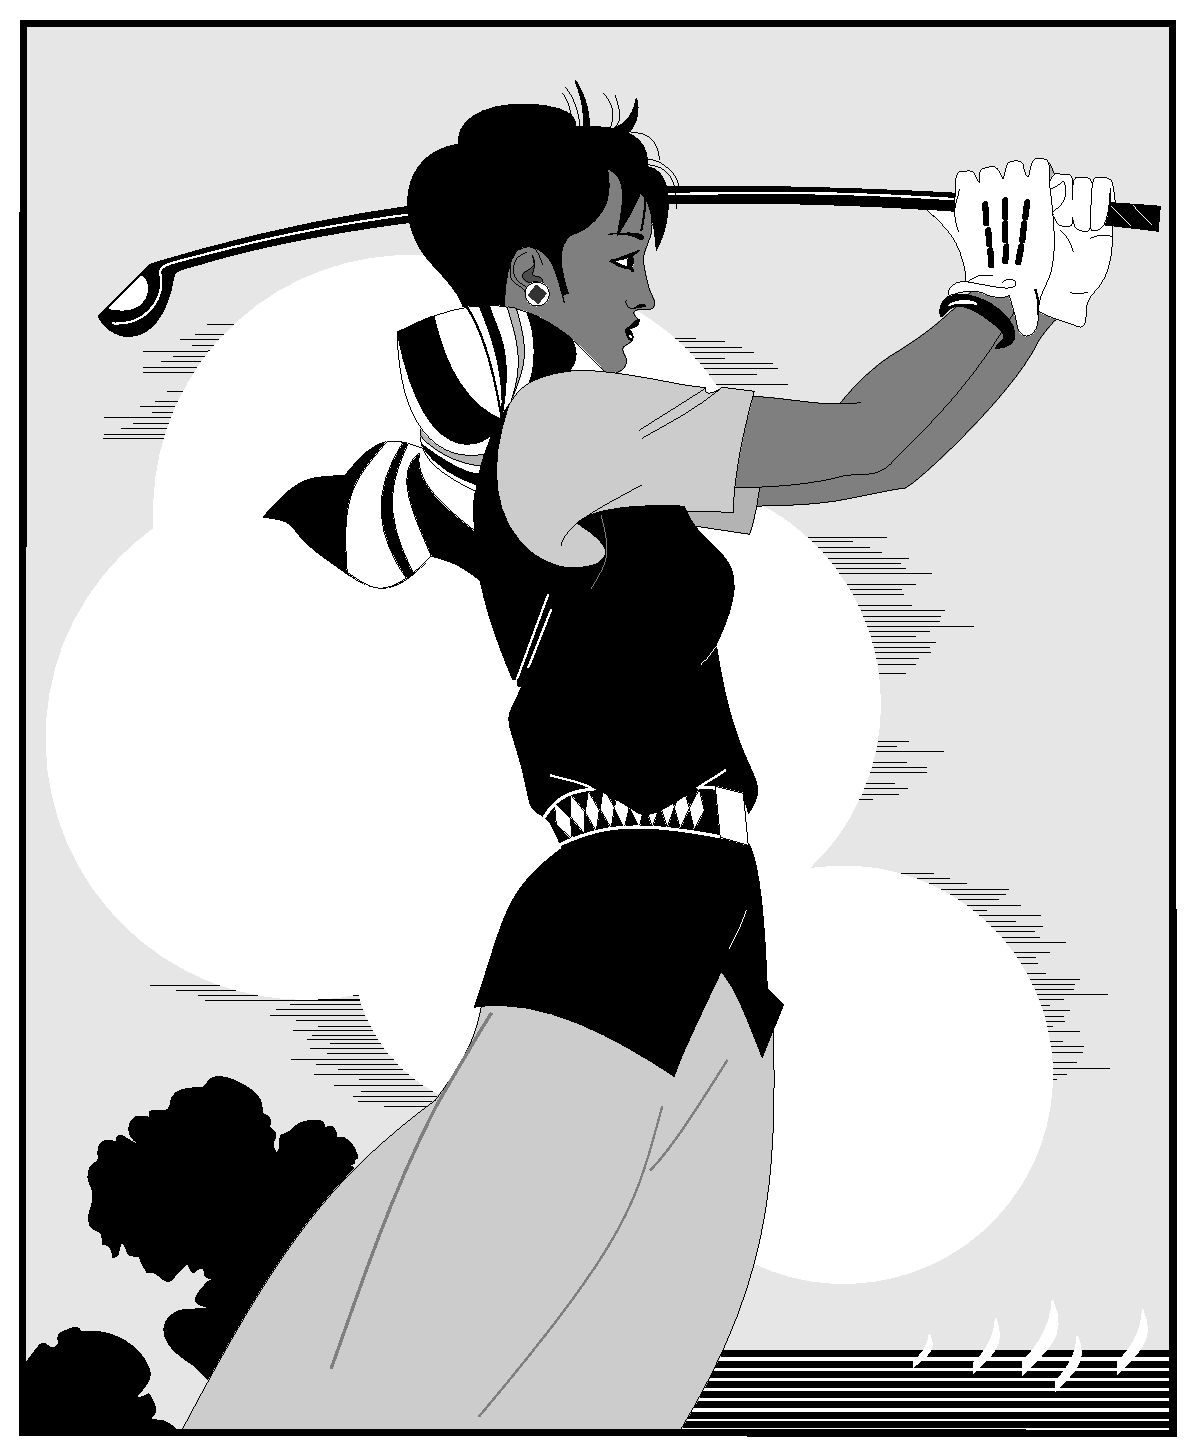
\includegraphics[width = \textwidth]{golfer}\vspace{-5mm}
\FigureBiCaption{��߶��������test}{Gor Golfer Golfer}
\label{Figure:Tricks:Example1211}
\end{minipage}\hspace{1cm}
\begin{minipage}[t]{0.4\textwidth}
\centering
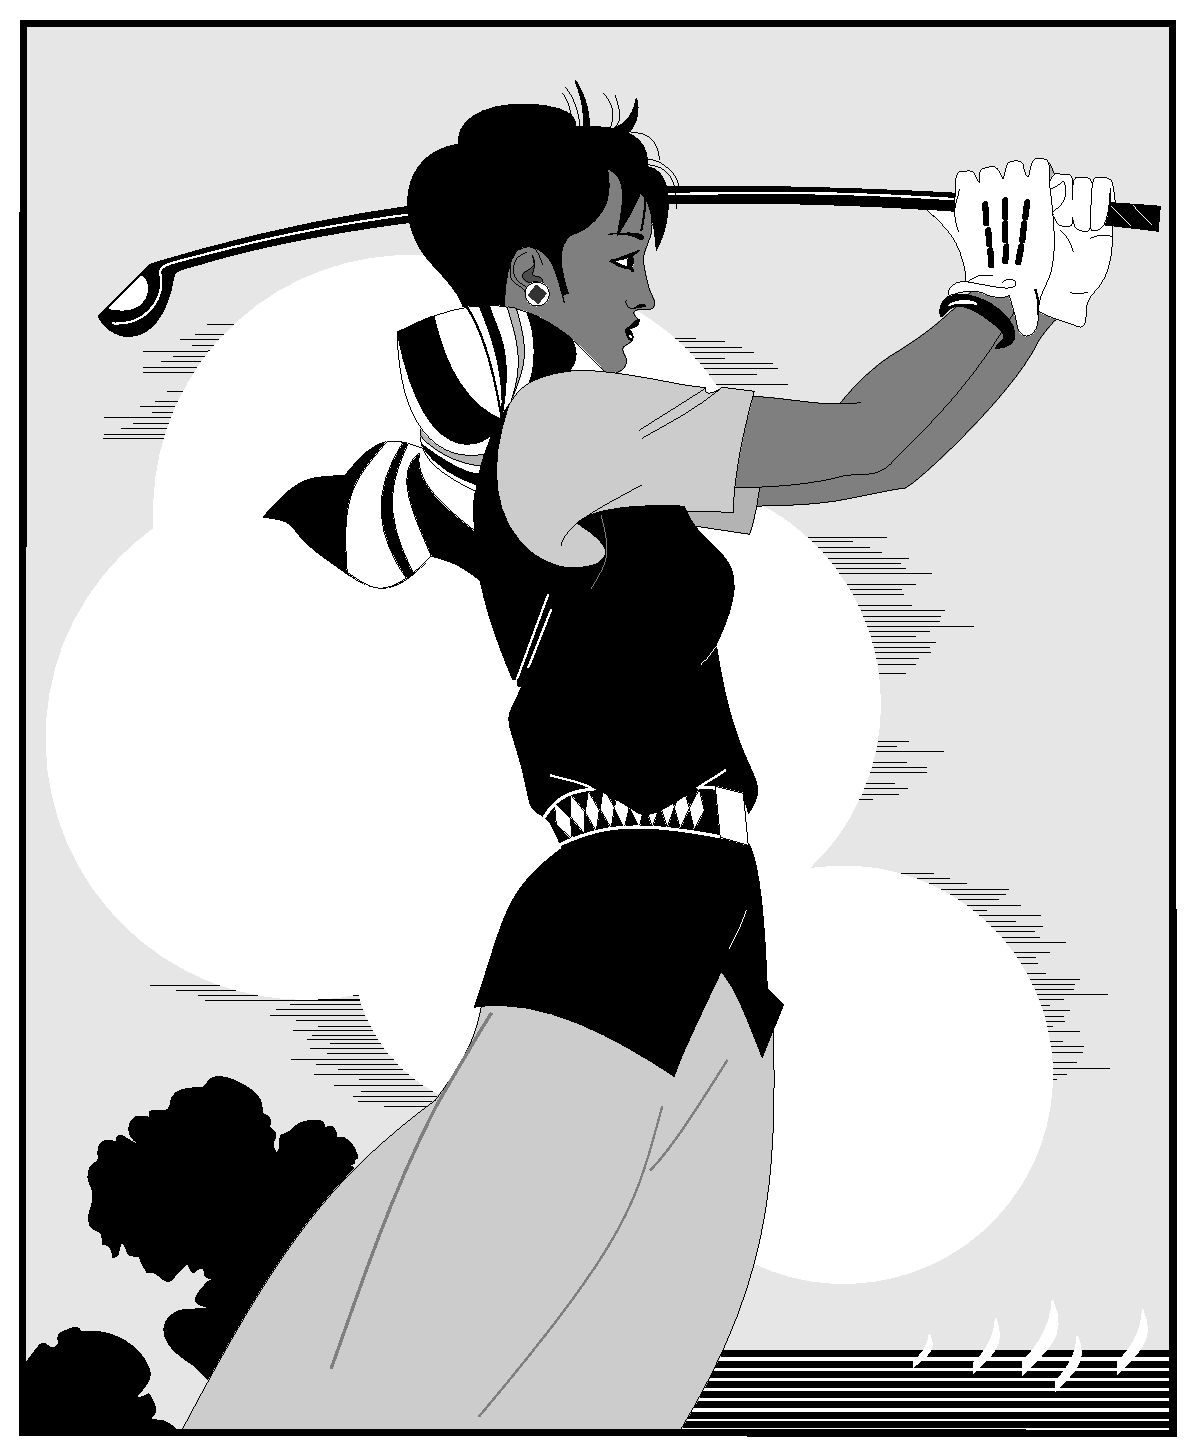
\includegraphics[width = \textwidth]{golfer}\vspace{-5mm}
\FigureBiCaption{��߶�����teste2}{Golfer Goolfer Golfer }
\label{Figure:Tricks:Example12222}
\end{minipage}
\end{figure}

% -*-coding: utf-8 -*-

\defaultfont

%%%%%%%%%%%%%%%%%%%%%%%%%%%%%%%%%%%%%%%%%%%%%%%%%%%%%%%%%%%%%%%%%%%%%%%%%%%%%
\BiChapter{版权声明}{Copyright Statement}

本模板遵循~GPL~协议。各贡献者在下面列出:\\
UFO\\
cucme\\
Stanley\\
TeX\\
nebula\\
luckyfox\\
jdg\\
LaTeX\\
还有许多校内校外热心提供帮助解决模板问题的网友朋友们。

% -*-coding: utf-8 -*-

\defaultfont

\BiAppendixChapter{结~~~~论}{Conclusion}
本文提供了一个~\LaTeX~学位论文模板及使用该模板的一些技巧。

如有什么问题,请到哈工大紫丁香~bbs~的~TeX~版发贴。
   % 结论

%参考文献
\defaultfont
\ifx\atempxetex\usewhat
\bibliographystyle{chinesebst2005_UTF8}
\else
\bibliographystyle{chinesebst2005_UTF8}
\fi
\addcontentsline{toc}{chapter}{\hei \ReferenceCName}      % 参考文献加入到中文目录
\addcontentsline{toe}{chapter}{\bfseries \sihao \ReferenceEName} % 参考文献加入到英文目录
\addtolength{\bibsep}{-0.8 em} \nocite{*}
\bibliography{reference/reference}

%\addtocontents{fen}{\protect\vskip1\baselineskip}
%\addtocontents{ten}{\protect\vskip1\baselineskip}
%英文图形和表格索引里加入空白行,通常放在 % -*-coding: utf-8 -*-

\defaultfont
\appendix

%%%%%%%%%%%%%%%%%%%%%%%%%%%%%%%%%%%%%%%%%%%%%%%%%%%%%%%%%
\BiAppChapter{带章节的附录}{Full Appendix}%
完整的附录内容,包含章节,公式,图表等

%%%%%%%%%%%%%%%%%%%%%%%%%%%%%%%%%%%%%%%%%%%%%%%%%%%%%%%%%
\BiSection{附录节的内容}{Section in Appendix}
这是附录的节的内容

附录中图的示例:
\begin{figure}[h]
\centering
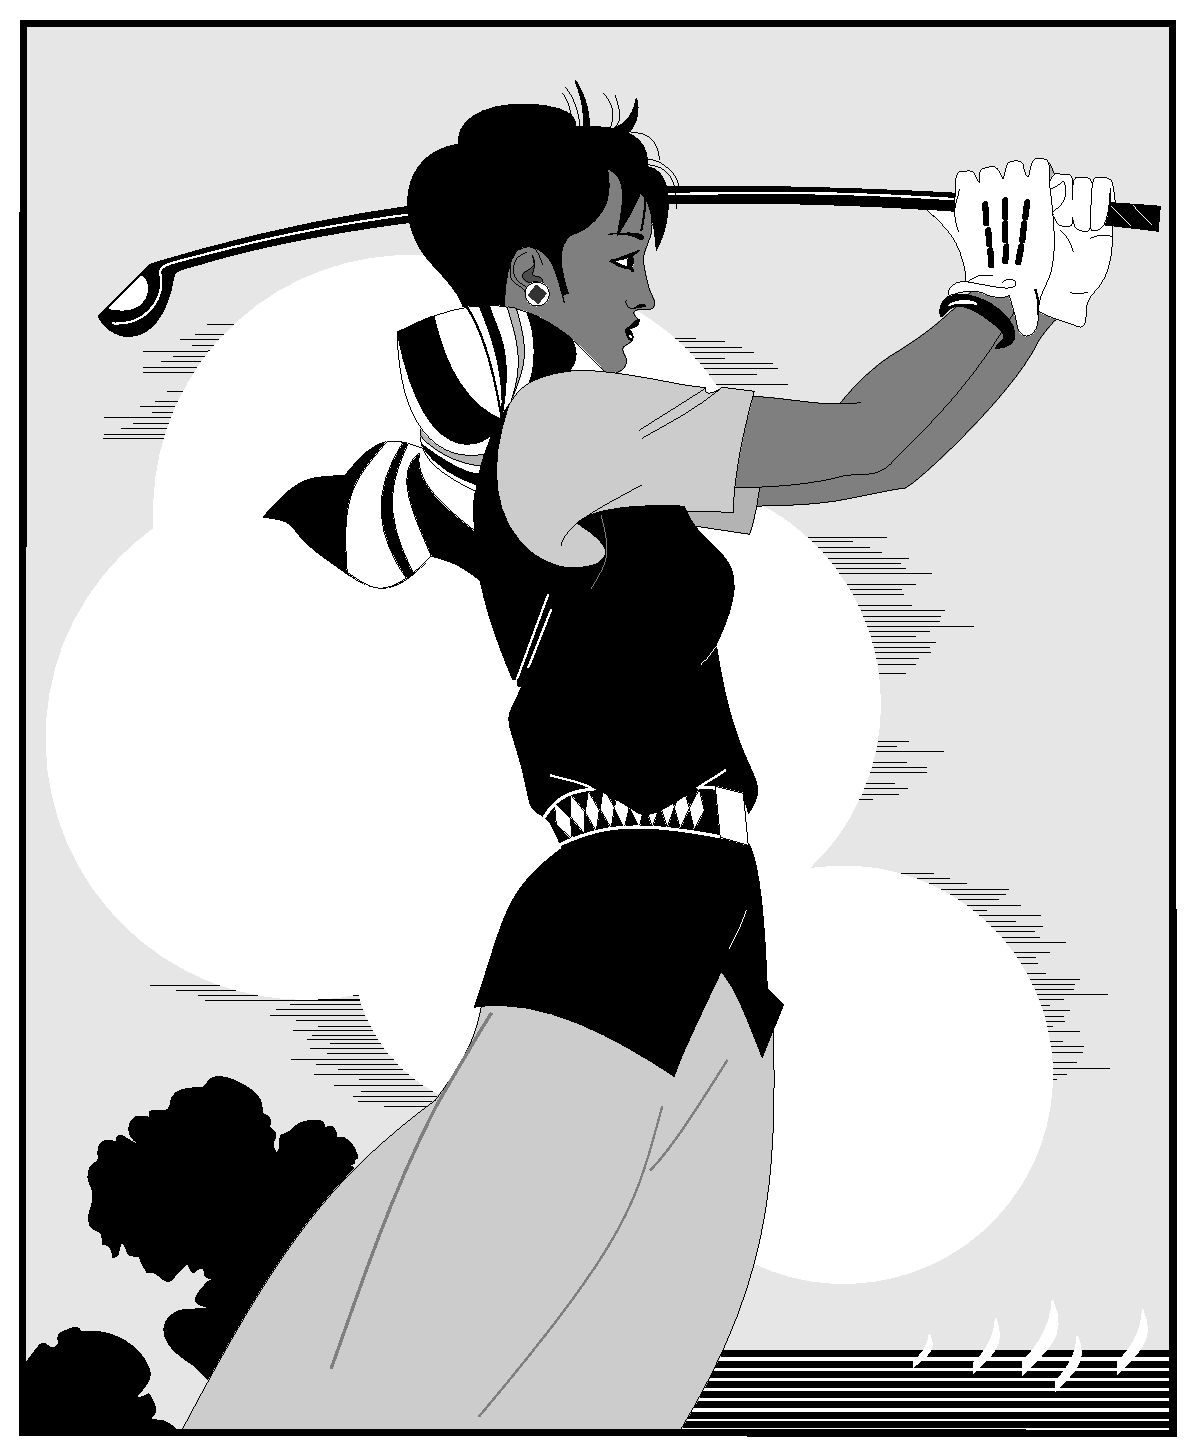
\includegraphics[width = 0.3\textwidth]{golfer}
\FigureBiCaption{打高尔夫球的人}{Golfer}
\label{Figure:Appendix:Example1}
\end{figure}

附录中公式的示例:
\begin{align}
a & = b \times c \\
E & = m c^2
\end{align}

%\BiAppChapter{附录二}{appendix 2}
%\BiAppChapter{附录三}{appendix 3}% 附录A之前。
%区分开正文和附录的图形和表格,一般没有这个必要。

% -*-coding: utf-8 -*-

\defaultfont
\appendix

%%%%%%%%%%%%%%%%%%%%%%%%%%%%%%%%%%%%%%%%%%%%%%%%%%%%%%%%%
\BiAppChapter{带章节的附录}{Full Appendix}%
完整的附录内容,包含章节,公式,图表等

%%%%%%%%%%%%%%%%%%%%%%%%%%%%%%%%%%%%%%%%%%%%%%%%%%%%%%%%%
\BiSection{附录节的内容}{Section in Appendix}
这是附录的节的内容

附录中图的示例:
\begin{figure}[h]
\centering
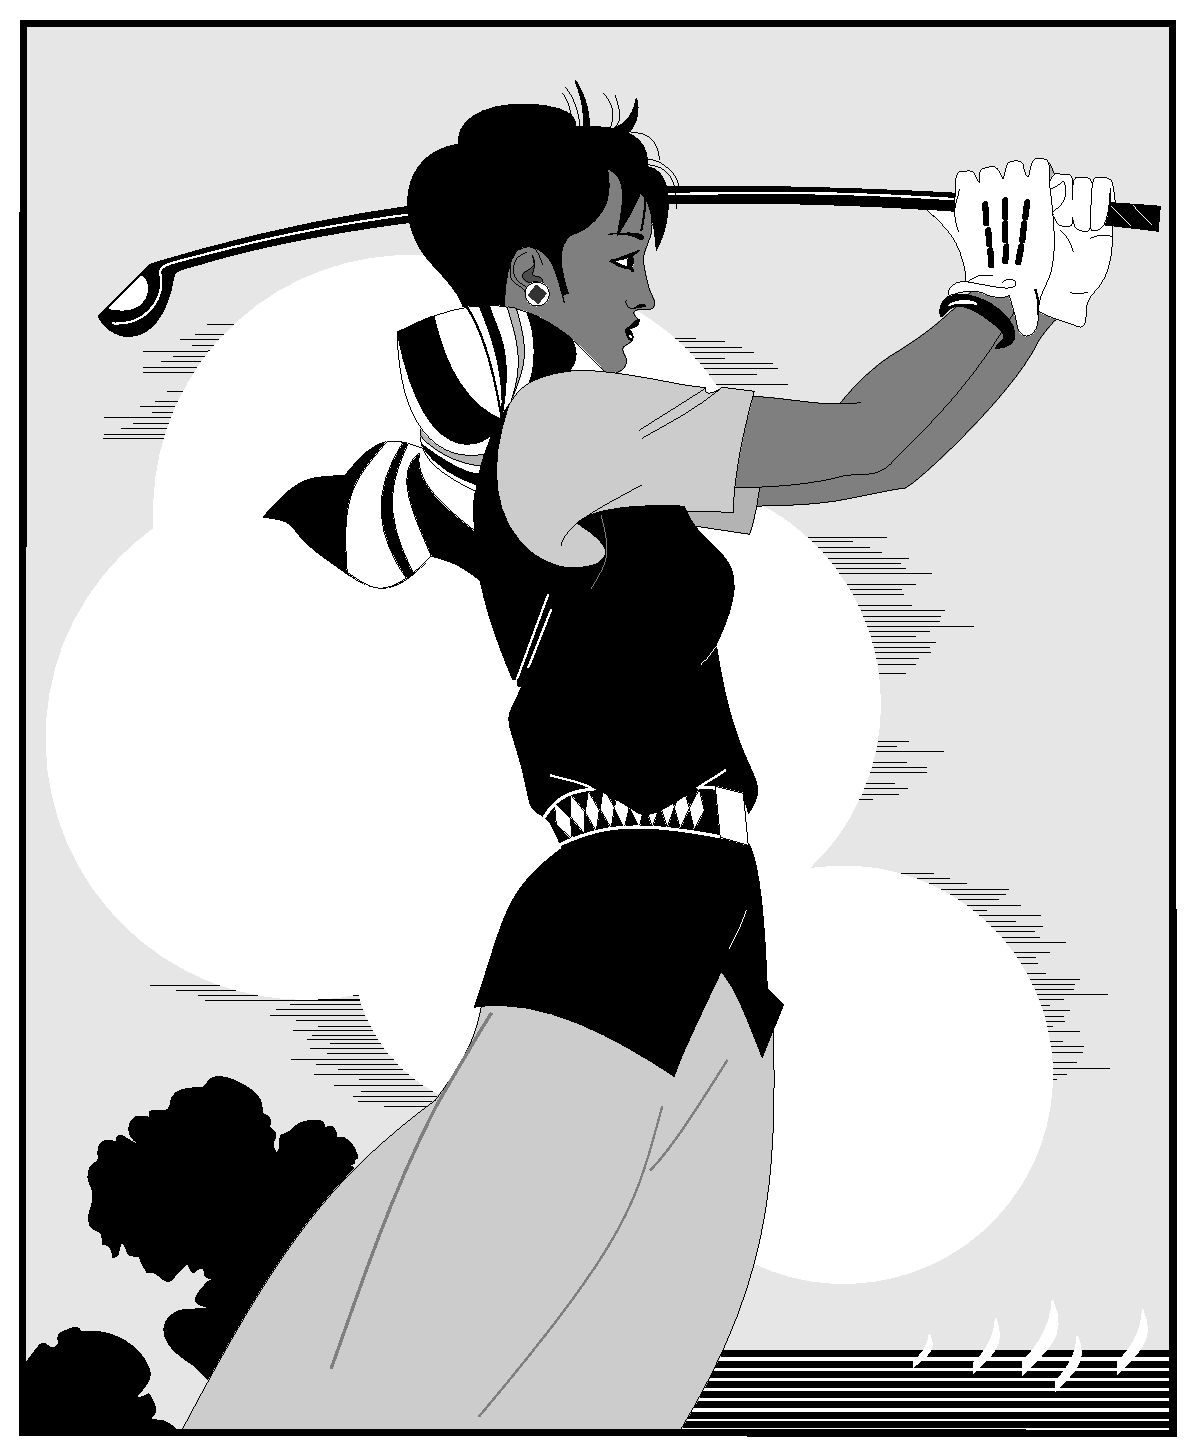
\includegraphics[width = 0.3\textwidth]{golfer}
\FigureBiCaption{打高尔夫球的人}{Golfer}
\label{Figure:Appendix:Example1}
\end{figure}

附录中公式的示例:
\begin{align}
a & = b \times c \\
E & = m c^2
\end{align}

%\BiAppChapter{附录二}{appendix 2}
%\BiAppChapter{附录三}{appendix 3}            % 附录A
\defaultfont
\BiAppendixChapter{����\cxueweiѧλ�ڼ�������������} {Papers
Published in the Period of PH. D. Education}

\begin{publist}
\item ����. ��Ŀ. �ڿ�. ��, ��(��): ҳ��

\item ����. ��Ŀ. �ڿ�. ��, ��(��): ҳ��

\item ����. ��Ŀ. �ڿ�. ��, ��(��): ҳ��
\end{publist}
    % 所发文章
% ��xelatex�����UTF8�ļ�������ÿ���ļ���ָ���ַ�����;
% main.tex���ֶ��ƶ���\atemp��\usewhat������
\ifx\atempxetex\usewhat 
\XeTeXinputencoding "gbk"
\fi
\defaultfont

\BiAppendixChapter{��~~~~л}{Acknowledgement}

������ģ����UFO@bbs.hit.edu.cn�ġ���������ҵ��ѧ��ѧ��ʿ��˶ʿ������ģ�塷�Ļ����ϣ�
���ںܶ��˵İ�������ɵģ��ڴ�һ�������DZ�ʾ��л��

�ر��лStanley����������ģ�忪Դ��ĿPluto�Լ���������ģ��Ĵ����޸ģ�
ʹ֮���ӷ��Ϲ�������ģ��Ҫ��

�ر��л�������϶���վ��~Tex~�İ���~Tex��nebula������cucme��
������ʼ���ն�ȫ��֧��ģ�����������Ϊ�����˴����Ĺ�����

��л���괺~(HIT bbs ID: dengnch)�������˴�����ʱ��������ģ���
һϵ�в�����ʹ�ø�~\LaTeX~ģ��Ͷ�Ӧ��~Word~ģ��ĸ�ʽ������ȫһ�¡�

��лˮľ�廪��~\TeX~��~\LaTeX~��ĸ�λ����Ϊ���ṩ�ĸ��ְ�����
�ر���~snoopyzhao~���ѣ���������ĵ�Ϊ��ģ�����������ѣ�ʹ��ģ�����������
˳�����С�

������ĸ�л�������϶���~bbs~վ~Tex~���������ѵĴ���֧�֣�



ֵ���������֮�ʣ������������˽��������ʦ��ͬѧ�����Գ�ֿ��л�⣡

���ȸ�л�ҵĵ�ʦ{\bf ijijij}���ڣ������ĵ��о�����������{\bf
ij}��ʦ����Ľ�����չ���ġ�
����ѧ���ϲ��Ͻ�ȡ������������ִ��׷��ľ�������ѧϰ�İ�����{\bf
ij}��ʦ��������̵���ʶ������dz���Ľ�������������ӡ��


��л{\bf ijijij}���ں�{\bf ijijij}���ڶ���ѧϰ�͹����İ�����
�����ڷܵĹ������硢��۵�����̬�ȶ�����ظ�Ⱦ���ҡ���л{\bf
ijijij}���ں�{\bf ijijij}���ڶ���ѧҵ�������ϵĹ��ġ�


��л��ʿ��{\bf ijijij}��{\bf ijijij}��{\bf ijijij}��{\bf ijijij}��
���ҵ���˽�����ͻ���֧�֡���лʵ�������е��ֵܽ����ǣ�
����Ҷȹ����ⳤ�õ�ѧϰ���о��׶Σ������ҽ�����⣬����˼�롣

����ر�Ҫ��л�ҵ������ǣ����Ƕ���Ҫ�����٣��������ҵĶ��ǹػ���֧�ֺ����⡣
% 致谢
% -*-coding: utf-8 -*-

% 先后有三个版本的 授权书格式


\iffalse   %注释掉第一个,采用第二个;
%  +++++++++ 下面是第一种处理方式  ++++++++++++++++++++++++++
    \newpage
%%%%%%%%%%%%%%%%%%哈尔滨工业大学博(硕)士学位论文原创性声明%%%%%%%%%%%%%%%%%%%
    \BiAppendixChapter{哈尔滨工业大学\cxuewei 学位论文原创性声明}{Statement of Copyright}

    本人郑重声明: 此处所提交的 \cxuewei 学位论文《\chinesethesistitle》,
    是本人在导师指导下, 在哈尔滨工业大学攻读\cxuewei 学位期间独立进行研究工作所取得的成果。据本人所知,论文中除已注明部分外不包含他人已发表或撰写过的研究成果。
    对本文的研究工作做出重要贡献的个人和集体, 均已在文中以明确方式注明。 本声明的
    法律结果将完全由本人承担。
    \vspace{0.5cm}
    \begin{flushright}{
    作者签名:~~~~~~~~~~~~~~~~~~~~~~~~~~~~~~~日期:~~~~~~~~~~~年~~~~~月~~~~~日}
    \end{flushright}

    \vspace{0.3cm}

%%%%%%%%%%%%%%%%%%哈尔滨工业大学博(硕)士学位论文使用授权书%%%%%%%%%%%%%%%%%%%
%\phantomsection
\addcontentsline{toc}{chapter}{\hei 哈尔滨工业大学\cxuewei 学位论文使用授权书}
\addcontentsline{toe}{chapter}{\bfseries Letter of Authorization}
    \begin{center}{\xiaoer \hei \bfseries
                    哈尔滨工业大学\cxuewei 学位论文使用授权书}
    \end{center}

    \vspace{0.4cm}

《\chinesethesistitle》 系本人在哈尔滨工业大学攻读\cxuewei 学位期
间在导师指导下完成的\cxuewei 学位论文。本论文的研究成果归哈尔滨工业大学所有,本
论文的研究内容不得以其它单位的名义发表。本人完全了解哈尔滨工业大学关于保存
、使用学位论文的规定,同意学校保留并向有关部门送交论文的复印件和电子版本,
允许论文被查阅和借阅,同意学校将论文加入《中国优秀博硕士学位论文全文数据库》和编入《中国知识资源总库》。本人授权哈尔滨工业大学,可以采用影印、缩印或其他复制
手段保存论文,可以公布论文的全部或部分内容。

\vspace{1.0cm}
\begin{flushright}{
作者签名:~~~~~~~~~~~~~~~~~~~~~~~~~~~~~~~日期:~~~~~~~~~~~年~~~~~月~~~~~日}
\end{flushright}
\vspace{0.2cm}
\begin{flushright}{
导师签名:~~~~~~~~~~~~~~~~~~~~~~~~~~~~~~~日期:~~~~~~~~~~~年~~~~~月~~~~~日}
\end{flushright}

\newpage

\BiAppendixChapter{哈尔滨工业大学\cxuewei 学位涉密论文管理}{Letter of Secret}

%    \begin{center}{\xiaoer \hei \bfseries
%                    哈尔滨工业大学硕博士学位涉密论文管理}
%    \end{center}
%    \vspace{0.4cm}
%\addcontentsline{toc}{chapter}{\hei 哈尔滨工业大学\cxuewei 学位涉密论文管理}
%\addcontentsline{toe}{chapter}{\bfseries Letter of Secret}

根据《哈尔滨工业大学关于国家秘密载体保密管理的规定》,毕业论文答辩必须由导师进行保密初审,外寄论文由科研处复审。涉密毕业论文,由学生按学校规定的统一程序在导师指导下填报密级和保密期限。

 \vspace{0.5cm}
~~~~~~~~~~~~~~~~~~~~~~~~~~~~~~~保密$\square$,在~~~~年解密后适用本授权书。

本学位论文属于

~~~~~~~~~~~~~~~~~~~~~~~~~~~~~~不保密 $\square$ 。

(请在以上相应方框内打“$\surd$”)
\vspace{1.0cm}

\begin{flushright}{
作者签名:~~~~~~~~~~~~~~~~~~~~~~~~~~~~~~~日期:~~~~~~~~~~~年~~~~~月~~~~~日}
\end{flushright} %\vspace{0.2cm}
\begin{flushright}{
导师签名:~~~~~~~~~~~~~~~~~~~~~~~~~~~~~~~日期:~~~~~~~~~~~年~~~~~月~~~~~日}
\end{flushright}

\fi  %注释掉第一个,采用第二个;

%+++++++++++++++++++++++第二种处理方式 by pineapple ++++++++++++++++++++++++++++++++
 \iffalse %% 如果不使用这种方式,去掉 \iffalse \fi 前面的注释
%%%%%%%%%%%%%%%%%%%%%%%%%%%%%%%%%%%%%%%%%%%%%%%%%%%%%%%%%%%%%%%%%%%%%%%%%%%%%%%%
% authorization.tex
%
% Authorization for Use with the Pluto Master Template
%
% Copyright (C) 2006 LIU Yu <pineapple.liu@gmail.com>
%
% This work may be distributed and/or modified under the conditions of the LaTeX
% Project Public License, either version 1.3 of this license or (at your option)
% any later version.
% The latest version of this license is in
%   http://www.latex-project.org/lppl.txt
% and version 1.3 or later is part of all distributions of LaTeX version
% 2005/12/01 or later.
%
% This work has the LPPL maintenance status `unmaintained'.
%
% This work consists of the file(s) authorization.tex
%%%%%%%%%%%%%%%%%%%%%%%%%%%%%%%%%%%%%%%%%%%%%%%%%%%%%%%%%%%%%%%%%%%%%%%%%%%%%%%%

\newpage
\markboth{哈尔滨工业大学\cxuewei 学位论文原创性声明}{哈尔滨工业大学\cxueke\cxuewei 学位论文}

\vspace*{0.1cm}
\newcommand{\subchapterstyle}%
  {\CJKfamily{hei}\rmfamily\bfseries\fontsize{16bp}{16bp}\selectfont}

%\phantomsection
\addcontentsline{toc}{chapter}{\hei 哈尔滨工业大学\cxuewei 学位论文原创性声明}
\addcontentsline{toe}{chapter}{\bfseries Statement of Copyright}
\begin{center}{\subchapterstyle 哈尔滨工业大学\cxuewei 学位论文原创性声明}\end{center}

    本人郑重声明:此处所提交的\cxuewei 学位论文《\chinesethesistitle》 ,是本人在导师指导下,在哈尔滨工业大学攻读\cxuewei 学位期间独立进行研究工作所取得的成果。据本人所知,论文中除已注明部分外不包含他人已发表或撰写过的研究成果。对本文的研究工作做出重要贡献的个人和集体,均已在文中以明确方式注明。本声明的法律结果将完全由本人承担。

\begin{flushright}

作者签字:~~~~~~~~~~~~~~~~~~~~~~~~~~~~~~~~~~~日期:~~~~~~~~~年~~~~~~月~~~~~~日~~~~

\end{flushright}

%\phantomsection
\addcontentsline{toc}{chapter}{\hei 哈尔滨工业大学\cxuewei 学位论文使用授权书}
\addcontentsline{toe}{chapter}{\bfseries Letter of Authorization}
\begin{center}{\subchapterstyle 哈尔滨工业大学\cxuewei 学位论文使用授权书}\end{center}

    《\chinesethesistitle》 系本人在哈尔滨工业大学攻读\cxuewei 学位期间在导师指导下完成的\cxuewei 学位论文。本论文的研究成果归哈尔滨工业大学所有,本论文的研究内容不得以其它单位的名义发表。本人完全了解哈尔滨工业大学关于保存、使用学位论文的规定,同意学校保留并向有关部门送交论文的复印件和电子版本,允许论文被查阅和借阅,同意学校将论文加入《中国优秀博硕士学位论文全文数据库》和编入《中国知识资源总库》。本人授权哈尔滨工业大学,可以采用影印、缩印或其他复制手段保存论文,可以公布论文的全部或部分内容。

\begin{flushright}

作者签名:~~~~~~~~~~~~~~~~~~~~~~~~~~~~~~~~~~~日期:~~~~~~~~~年~~~~~~月~~~~~~日~~~~

导师签名:~~~~~~~~~~~~~~~~~~~~~~~~~~~~~~~~~~~日期:~~~~~~~~~年~~~~~~月~~~~~~日~~~~

\end{flushright}

%\phantomsection
\addcontentsline{toc}{chapter}{\hei 哈尔滨工业大学\cxuewei 学位涉密论文管理} %研究生院说明:暂时不要添加到目录中去,
\addcontentsline{toe}{chapter}{\bfseries Letter of Secret}              %格式也没有完全规定,这里放到下一页上。

\begin{center}{\subchapterstyle 哈尔滨工业大学\cxuewei 学位涉密论文管理}\end{center}

    根据《哈尔滨工业大学关于国家秘密载体保密管理的规定》,毕业论文答辩必须由导师进行保密初审,外寄论文由科研处复审。涉密毕业论文,由学生按学校规定的统一程序在导师指导下填报密级和保密期限。

\begin{flushright}

本学位论文属于~~~~~~~~~~~~~~~~~~~保密$\square$,在~~~~~~~~~~~~年解密后适用本授权书。~~~~~

不保密
$\square$。~~~~~~~~~~~~~~~~~~~~~~~~~~~~~~~~~~~~~~~~~~~~~~~~~~~~~~~~~~~~~~

(请在以上相应方框内打“$\surd$”)~~~~~~~~~~~~~~~~~~~~~~~~~~~~~~~~~~~~~~~~~~~~~~~~~~~~~~~~~~~~~~~~~~~~~~~

\end{flushright}
\begin{flushright}

作者签名:~~~~~~~~~~~~~~~~~~~~~~~~~~~~~~~~~~~日期:~~~~~~~~~年~~~~~~月~~~~~~日~~~~

导师签名:~~~~~~~~~~~~~~~~~~~~~~~~~~~~~~~~~~~日期:~~~~~~~~~年~~~~~~月~~~~~~日~~~~

\end{flushright}
 \fi

%% 第三种处理方式  author: jdg
% \iffalse
\newpage
\markboth{哈尔滨工业大学\cxuewei 学位论文原创性声明}{哈尔滨工业大学\cxueke\cxuewei 学位论文}

\vspace*{0cm}
\newcommand{\subchapterstyle}%
  {\CJKfamily{hei}\rmfamily\bfseries\fontsize{16bp}{16bp}\selectfont}

%\phantomsection
\addcontentsline{toc}{chapter}{\hei 哈尔滨工业大学\cxuewei 学位论文原创性声明}
\addcontentsline{toe}{chapter}{\bfseries Statement of Copyright}
\begin{center}{\subchapterstyle 哈尔滨工业大学\cxuewei 学位论文原创性声明}\end{center}

    本人郑重声明:此处所提交的\cxuewei 学位论文《\chinesethesistitle》 ,是本人在导师指导下,在哈尔滨工业大学攻读\cxuewei 学位期间独立进行研究工作所取得的成果。据本人所知,论文中除已注明部分外不包含他人已发表或撰写过的研究成果。对本文的研究工作做出重要贡献的个人和集体,均已在文中以明确方式注明。本声明的法律结果将完全由本人承担。

\begin{flushright}

作者签名:~~~~~~~~~~~~~~~~~~~~~~~~~~~~~~~~~~~日期:~~~~~~~~~年~~~~~~月~~~~~~日~~~~

\end{flushright}

\vspace{0.4cm}
%\phantomsection
\addcontentsline{toc}{chapter}{\hei 哈尔滨工业大学\cxuewei 学位论文使用授权书}
\addcontentsline{toe}{chapter}{\bfseries Letter of Authorization}
\begin{center}{\subchapterstyle 哈尔滨工业大学\cxuewei 学位论文使用授权书}\end{center}

    《\chinesethesistitle》 系本人在哈尔滨工业大学攻读\cxuewei 学位期间在导师指导下完成的\cxuewei 学位论文。本论文的研究成果归哈尔滨工业大学所有,本论文的研究内容不得以其它单位的名义发表。本人完全了解哈尔滨工业大学关于保存、使用学位论文的规定,同意学校保留并向有关部门送交论文的复印件和电子版本,允许论文被查阅和借阅,同意学校将论文加入《中国优秀博硕士学位论文全文数据库》和编入《中国知识资源总库》。本人授权哈尔滨工业大学,可以采用影印、缩印或其他复制手段保存论文,可以公布论文的全部或部分内容。

\vspace{0.6cm}
本学位论文属于(请在以下相应方框内打“$\surd$”):

保密$\square$,在~~~~~~~~~~~~~年解密后适用本授权书

不保密$\square$

\begin{flushright}{
作者签名:~~~~~~~~~~~~~~~~~~~~~~~~~~~~~~~~~~~日期:~~~~~~~~~年~~~~~~月~~~~~~日~~~~}
\end{flushright} %\vspace{0.2cm}
\begin{flushright}{
导师签名:~~~~~~~~~~~~~~~~~~~~~~~~~~~~~~~~~~~日期:~~~~~~~~~年~~~~~~月~~~~~~日~~~~}
\end{flushright}
%\fi   % 承诺
% -*-coding: utf-8 -*-

\defaultfont

\BiAppendixChapter{个人简历}{Resume}

{\hei 学习经历}
\begin{publist}
\item xxxx~年~x~月--至今~~哈尔滨工业大学xxxxxxxxx系~~~攻读工学博士学位
\item xxxx~年~x~月~~~xxxxxxx大学xxxxxxxxxxxxxxxxxx系~~~获工学硕士学位
\item xxxx~年~x~月~~~xxxxxxx大学xxxxxxxxxxxxxxxxxx系~~~获工学学士学位
\end{publist}

{\hei 工作经历}
\begin{publist}
\item xxxx~年~x~月--xxxx~年~x~月  单位  职务
\item xxxx~年~x~月--xxxx~年~x~月  单位  职务
\end{publist}

{\hei 科研工作}
\begin{publist}
\item  xxxx~年~x~月--xxxx~年~x~月 ~~~ xxxx项目~~~~(编号xxx-xxx-xxx) 
\item  xxxx~年~x~月--xxxx~年~x~月 ~~~ xxxx项目~~~~(编号xxx-xxx-xxx)
\item  xxxx~年~x~月--xxxx~年~x~月 ~~~ xxxx项目~~~~(编号xxx-xxx-xxx)
\item  xxxx~年~x~月--xxxx~年~x~月 ~~~ xxxx项目~~~~(编号xxx-xxx-xxx)
\end{publist}

{\hei 学术论文}
\begin{publist}
\item 在~xxxxxxx~等刊物发表论文多篇
\item 在~xxxxxxxxxxxxxxxx~等多个国际会议上发表论文多篇
\end{publist}

{\hei 专利情况}
\begin{publist}
\item 作者. 产品名称. 专利名称(专利号:XXXXXXX), 年。
\item 作者. 产品名称. 专利名称(专利号:XXXXXXX), 年。
\end{publist}
          % 个人简历

\clearpage
\ifx\atempxetex\usewhat\else
\end{CJK*}
\fi

\end{document}

%%% Local Variables: 
%%% mode: latex
%%% TeX-master: t
%%% End: 
